%%%%%%%%%%%%%%%%%%%%%%%%%%%%%%%%%%%%%%%%%%
%                                        %
% Szablon pracy dyplomowej magisterskiej % 
%                                        %
%%%%%%%%%%%%%%%%%%%%%%%%%%%%%%%%%%%%%%%%%%

\documentclass[a4paper,twoside,12pt]{book}
\usepackage[utf8]{inputenc}                                      
\usepackage[T1]{fontenc}  
\usepackage{amsmath,amsfonts,amssymb,amsthm}
\usepackage[british,polish]{babel} 
\usepackage{indentfirst}
\usepackage{lmodern}
\usepackage{graphicx} 
\usepackage{hyperref}
\usepackage{booktabs}
%\usepackage{tikz}
%\usepackage{pgfplots}
\usepackage{mathtools}
\usepackage{geometry}
\usepackage[page]{appendix} % toc,

\renewcommand{\appendixtocname}{Dodatki}
\renewcommand{\appendixpagename}{Dodatki}
\renewcommand{\appendixname}{Dodatek}

\usepackage{setspace}
\onehalfspacing

% Paczki dotyczące tabel
\usepackage{tabularx}
\usepackage{makecell}
% Kolorowanie tabeli
\usepackage[table]{xcolor}
% Odstęp przy nazwie tabeli
\usepackage{caption}
\captionsetup[table]{skip=10pt}
% Nazwa "Tabela" zamiast "Tablica"
\captionsetup[table]{name=Tabela}

% Proste cudzysłowy
\usepackage{textcomp}

% Pogrubione sigma
\usepackage{bm}


\frenchspacing

\usepackage{listings}
\lstset{
	basicstyle=\ttfamily,
	keywordstyle=\lst@ifdisplaystyle\color{blue}\fi,
	commentstyle=\color{gray},
    numbers = left, %% display line numbers on the left
    breaklines = true, %% enable line breaking
    frame = lines,
    aboveskip = 15pt,
    belowskip = 5pt,
    showstringspaces = false
}
\lstdefinestyle{SQL} {
    language=SQL,
    morecomment=[f][\color{gray}][0]{\%},
}

\lstdefinestyle{SQL-with-inline-comments} {
    language=SQL,
    morecomment=[l][\color{gray}]{\%},
}

\renewcommand{\lstlistingname}{Kod}% Listing -> Kod



%%%%%%%%%

%%%% TODO LIST GENERATOR %%%%%%%%%

%\usepackage{tikz}
%\usepackage{manfnt}   % dangerous sign 
\usepackage{color}
\definecolor{brickred}      {cmyk}{0   , 0.89, 0.94, 0.28}

\makeatletter \newcommand \kslistofremarks{\section*{Uwagi} \@starttoc{rks}}
  \newcommand\l@uwagas[2]
    {\par\noindent \textbf{#2:} %\parbox{10cm}
{#1}\par} \makeatother


\newcommand{\ksremark}[1]{%
{%\marginpar{\textdbend}
{\color{brickred}{[#1]}}}%
\addcontentsline{rks}{uwagas}{\protect{#1}}%
}

\newcommand{\comma}{\ksremark{przecinek}}
\newcommand{\nocomma}{\ksremark{bez przecinka}}
\newcommand{\styl}{\ksremark{styl}}
\newcommand{\ortografia}{\ksremark{ortografia}}
\newcommand{\fleksja}{\ksremark{fleksja}}
\newcommand{\pauza}{\ksremark{pauza `--', nie dywiz `-'}}
\newcommand{\kolokwializm}{\ksremark{kolokwializm}}

%%%%%%%%%%%%%% END OF TODO LIST GENERATOR %%%%%%%%%%%

%%%%%%%%%%%% ZYWA PAGINA %%%%%%%%%%%%%%%
% brak kapitalizacji zywej paginy
\usepackage{fancyhdr}
\pagestyle{fancy}
\fancyhf{}
\fancyhead[LO]{\nouppercase{\it\rightmark}}
\fancyhead[RE]{\nouppercase{\it\leftmark}}
\fancyhead[LE,RO]{\it\thepage}


\fancypagestyle{tylkoNumeryStron}{%
   \fancyhf{} 
   \fancyhead[LE,RO]{\it\thepage}
}

\fancypagestyle{NumeryStronNazwyRozdzialow}{%
   \fancyhf{} 
   \fancyhead[LO]{\nouppercase{\it\rightmark}}
   \fancyhead[RE]{\nouppercase{\it\leftmark}}
   \fancyhead[LE,RO]{\it\thepage}
}


%%%%%%%%%%%%% OBCE WTRETY  
\newcommand{\obcy}[1]{\emph{#1}}
\newcommand{\ang}[1]{{\selectlanguage{british}\obcy{#1}}}
%%%%%%%%%%%%%%%%%%%%%%%%%%%%%

% polskie oznaczenia funkcji matematycznych
\renewcommand{\tan}{\operatorname {tg}}
\renewcommand{\log}{\operatorname {lg}}

% jeszcze jakies drobiazgi

\newcounter{stronyPozaNumeracja}

\newcommand{\hcancel}[1]{%
    \tikz[baseline=(tocancel.base)]{
        \node[inner sep=0pt,outer sep=0pt] (tocancel) {#1};
        \draw[red] (tocancel.south west) -- (tocancel.north east);
    }%
}%

\newcommand{\miesiac}{%
  \ifcase\the\month
  \or styczeń% 1
  \or luty% 2
  \or marzec% 3
  \or kwiecień% 4
  \or maj% 5
  \or czerwiec% 6
  \or lipiec% 7
  \or sierpień% 8
  \or wrzesień% 9
  \or październik% 10
  \or listopad% 11
  \or grudzień% 12
  \fi}


%%%%%%%%%%%%%%%%%%%%%%%%%%%%%%%%%%%%%%%%%%%%%%
% Helvetica font macros for the title page:
\newcommand{\headerfont}{\fontfamily{phv}\fontsize{18}{18}\bfseries\scshape\selectfont}
\newcommand{\titlefont}{\fontfamily{phv}\fontsize{18}{18}\selectfont}
\newcommand{\otherfont}{\fontfamily{phv}\fontsize{14}{14}\selectfont}

%%%%%%%%%%%%%%%%%%%%%%%%%%%%%%%%%%%%%%%%%%%%%%
%%%%%%%%%%%%%%%%%%%%%%%%%%%%%%%%%%%%%%%%%%%%%%
%%%%%%%%%%%%%%%%%%%%%%%%%%%%%%%%%%%%%%%%%%%%%%
%%%%%%%%%%%%%%%%%%%%%%%%%%%%%%%%%%%%%%%%%%%%%%
%%%%%%%%%%%%%%%%%%%%%%%%%%%%%%%%%%%%%%%%%%%%%%
%%%%%%%%%%%%%%%%%%%%%%%%%%%%%%%%%%%%%%%%%%%%%%
%%%%%%%%%%%%%%%%%%%%%%%%%%%%%%%%%%%%%%%%%%%%%%


\newcommand{\autor}{inż. Krzysztof Sobocik}
\newcommand{\promotor}{dr inż. Ewa Płuciennik}
% \newcommand{\konsultant}{tytul/stopien naukowy Imię Nazwisko}
\newcommand{\tytul}{Analiza cech obiektowych w relacyjnych bazach danych}
\newcommand{\polsl}{Politechnika Śląska}
\newcommand{\wydzial}{Wydział Automatyki, Elektroniki i Informatyki}
\newcommand{\kierunek}{Kierunek: Informatyka}

\begin{document}
%\kslistofremarks 
	
%%%%%%%%%%%%%%%%%%  STRONA TYTULOWA %%%%%%%%%%%%%%%%%%%
\pagestyle{empty}
{
	\newgeometry{top=2.5cm,%
	             bottom=2.5cm,%
	             left=3cm,
	             right=2.5cm}
	\sffamily
	\rule{0cm}{0cm}
	
	\begin{center}
	
\includegraphics[width=45mm]{logo.jpg}
	\end{center} 
	\vspace{1cm}
	\begin{center}
	\headerfont \polsl
	\end{center}
	\begin{center}
	\headerfont \wydzial
	\end{center}
	\begin{center}
	\headerfont \kierunek
	\end{center}
	\vfill
	\begin{center}
	\titlefont Praca dyplomowa magisterska
	\end{center}
	\vfill
	
	\begin{center}
	\otherfont \tytul\par
	\end{center}
	
	\vfill
	
	\vfill
	 
	\noindent\vbox
	{
		\hbox{\otherfont Autor: \autor}
		\vspace{12pt}
		\hbox{\otherfont Promotor: \promotor}
% 		\vspace{12pt}
% 		\hbox{\otherfont Konsultant: \konsultant}
	}
	\vfill 
 
   \begin{center}
   \otherfont Gliwice,  \miesiac\ \the\year
   \end{center}	
	\restoregeometry
}
  

\cleardoublepage
 

\rmfamily
\normalfont



%%%%%%%%%%%%%%%%%% SPIS TRESCI %%%%%%%%%%%%%%%%%%%%%%
\pagenumbering{Roman}
\pagestyle{tylkoNumeryStron}
\tableofcontents

%%%%%%%%%%%%%%%%%%%%%%%%%%%%%%%%%%%%%%%%%%%%%%%%%%%%%
\setcounter{stronyPozaNumeracja}{\value{page}}
\mainmatter


\pagestyle{empty}

\chapter*{Streszczenie}

Celem pracy jest analiza cech obiektowych występujących w dostępnych na rynku bazach danych. Na początku pracy przybliżono tematykę relacyjnych, obiektowych i obiektowo-relacyjnych systemów zarządzania bazami danych. Omówiono także paradygmat programowania obiektowego i jego wpływ na rozwój baz danych. Następnie przedstawiono dostępne na rynku systemy obiektowo-relacyjne i szczegółowo przeanalizowano mechanizmy trzech systemów: Oracle Database, IBM Db2 i PostgreSQL. Przedstawiono wszystkie istotne cechy obiektowe dostępne w analizowanych systemach i przeprowadzono ich porównanie z rozwiązaniami opisanymi w standardzie SQL.

W ramach badań, w każdym systemie zaprojektowano obiektowo-relacyjną strukturę bazy danych dla dziedziny hurtowni sprzętów elektronicznych. Projektując model bazy wykorzystano jak najwięcej spośród dostępnych mechanizmów obiektowych. W każdym systemie stworzono także standardową strukturę relacyjną dla tej samej dziedziny. Korzystając ze stworzonej aplikacji, wygenerowano zbiór danych i skrypty wstawiające dane do każdej bazy. Dla wszystkich struktur przygotowano i wykonano zapytania realizujące przykładowe wymogi biznesowe. Porównano treści zapytań dla różnych struktur i czasy ich wykonania. Pracę zamykają wnioski z~badań i syntetyczne podsumowanie analizy.

{\bf Slowa kluczowe:} bazy danych, relacyjne bazy danych, obiektowo-relacyjne bazy danych, paradygmat obiektowy, programowanie obiektowe, ORDBMS, SQL, Oracle, Db2, Postgres

\addcontentsline{toc}{chapter}{Streszczenie}

\cleardoublepage

\pagestyle{NumeryStronNazwyRozdzialow}
%%%%%%%%%%%%%% wlasciwa tresc pracy %%%%%%%%%%%%%%%%%


\chapter{Wstęp}

Postępujący rozwój technik analizy danych i szeroko pojętego \textit{data science} powoduje, że bazy danych stają się coraz bardziej istotne w systemach informatycznych. Powstaje wiele nowych modeli baz danych, a istniejące systemy poszerzają swoje możliwości by nadążyć za potrzebami rynku. Jednym z najpopularniejszych trendów w informatyce jest podejście obiektowe, czego efekty spotykane są także w systemach bazodanowych. Do dziś, najczęściej stosowanym modelem bazy jest model relacyjny, jednak wiele z najpopularniejszych systemów tego typu wprowadziło do swoich rozwiązań dodatkowe cechy obiektowe, rozszerzające standardowe możliwości bazy. Systemy wspierające mechanizmy obiektowe realizują tak zwany model obiektowo-relacyjny.

Celem niniejszej pracy magisterskiej jest przeanalizowanie cech obiektowych występujących w dostępnych na rynku relacyjnych bazach danych. Omówiony został paradygmat programowania obiektowego oraz jego wpływ na systemy bazodanowe. Przedstawiono charakterystykę relacyjnych, obiektowych i obiektowo-relacyjnych systemów zarządzania bazami danych. Szczegółowo rozpatrywane są mechanizmy obiektowe dostępne w systemach Oracle Database, IBM Db2 oraz PostgreSQL, a~także rozwiązania opisane w ramach standardu SQL.

W ramach badań, w każdej bazie stworzono porównywalne struktury obiektowo-relacyjne, opierając się na przykładowej fikcyjnej dziedzinie biznesowej. Dla stworzonych struktur przygotowano zbiór danych i przetestowano działanie baz za pomocą zróżnicowanych zapytań. Poszczególne systemy porównywane są pomiędzy sobą, a~także względem standardowego rozwiązania relacyjnego, stworzonego w~tej samej technologii. Badania mają na celu sprawdzenie przydatności dostępnych mechanizmów obiektowych i problemów spotykanych przy ich stosowaniu.

Praca składa się z 6 rozdziałów. Rozdział drugi stanowi wprowadzenie do analizowanego tematu oraz nakreślenie historycznej i obecnej pozycji podejścia obiektowego w bazach danych. Rozdział trzeci przybliża rozpatrywane w pracy systemy zarządzania bazą danych. Rozdział czwarty rozpatruje poszczególne mechanizmy obiektowe, ich opis w standardzie SQL i sposób ich implementacji w analizowanych systemach. W rozdziale piątym opisane są badania i testy rozwiązań obiektowych, które przeprowadzono z wykorzystaniem wybranych baz danych. Pracę zamyka podsumowanie zawierające wnioski końcowe z przeprowadzonej analizy.

\chapter{Analiza tematu}

Bazy danych są podstawą wielu systemów informatycznych, od najprostszych aplikacji mobilnych, przez sieciowe portale społecznościowe, aż po ogromne hurtownie danych nastawione na badania analityczne. Są dziś domyślnym rozwiązaniem dla przechowywania danych, naturalną ewolucją utrwalania danych w prostych plikach tekstowych.

Można wyróżnić wiele rodzajów baz danych. Standardowym rozwiązaniem są bazy relacyjne, używane z sukcesem od wielu lat. W ostatnich czasach popularnością cieszą się również szeroko pojęte bazy NoSQL, do których zalicza się większość systemów nierelacyjnych, takich jak bazy dokumentowe, grafowe czy kolumnowe. Dostępność wielu alternatywnych rozwiązań pozwala twórcom systemów informatycznych na dobór modelu bazy najbardziej dopasowanego do rozwiązywanego problemu domenowego i wymogów systemu \cite{bib:survey-and-comparison-of-rel-and-non-rel-databases}.

Warto zaznaczyć różnicę między bazą danych, a SZBD, czyli systemem zarządzania bazą danych. Precyzyjnie mówiąc, baza danych to zbiór powiązanych ze sobą informacji, przechowywanych w uporządkowanej strukturze, zwykle w formie elektronicznej, a SZBD to oprogramowanie umożliwiające pracę z tą bazą. Zapewnia komunikację z bazą danych i pełni rolę interfejsu, przez który użytkownik wykonuje wszelkie akcje na zbiorze danych. Najczęściej określenie ``baza danych'' odnosi się do kompletu bazy jako zbioru informacji i towarzyszącego mu systemu zarządzania - takie znaczenie tego pojęcia będzie najczęściej spotykane w ramach niniejszej pracy \cite{bib:evolution-odbs}. 

W tym rozdziale omówione zostaną trzy typy baz danych istotne dla tematu pracy, czyli bazy relacyjne, obiektowe i ostatecznie obiektowo-relacyjne, łączące cechy obydwu tych podejść. Zostanie przedstawione ich pochodzenie oraz różnice w ich działaniu. Jako wprowadzenie do baz obiektowych i obiektowo-relacyjnych zostanie przybliżony paradygmat programowania obiektowego i jego założenia.

\section{Relacyjne bazy danych}

Relacyjne bazy danych są najczęściej stosowanym rodzajem bazy danych. Według rankingu DB-Engines na rok 2021, cztery najpopularniejsze bazy na świecie wykorzystują model relacyjny, a w pierwszej dziesiątce są tylko trzy bazy o innym modelu \cite{bib:db-engines-ranking}. Popularność baz relacyjnych wynika w dużej mierze z ich silnych podstaw teoretycznych i przyzwyczajenia wykształconego w środowiskach programistycznych - przez wiele lat były dominującym rozwiązaniem, gdy alternatywy nie oferowały wystarczających zalet.

Autorem teoretycznych podstaw relacyjnych baz danych jest Edgar F. Codd, który w 1970 po raz pierwszy użył tego określenia w swojej pracy ``\textit{A Relational Model of Data for Large Shared Data Banks}''. Określił w niej tzw. ``Dwanaście Reguł Codd'a'', które definiują wymagania stawiane wobec Relacyjnych Systemów Zarządzania Bazą Danych (RSZBD). Dzisiejsze systemy relacyjne na ogół realizują tylko część spośród wszystkich reguł Codd'a \cite{bib:codd-relational-model-of-data}.

Model relacyjny realizuje intuicyjny sposób przechowywania danych, poprzez grupowanie danych w relacje reprezentowane przez tabele. Każda relacja, a więc także tabela, posiada unikatową nazwę, zbiór atrybutów oraz zawartość w postaci zbioru krotek. Atrybuty reprezentowane są przez kolumny tabeli, a krotki to poszczególne wiersze. Unikalnym identyfikatorem krotki jest tzw. klucz główny, czyli atrybut lub zbiór atrybutów o niepowtarzalnej wartości w danej tabeli. Zależności pomiędzy danymi przechowywanymi w różnych tabelach reprezentowane są za pomocą kluczy obcych, czyli atrybutów przechowujących wartości kluczy innych krotek.

Ogromną zaletą modelu relacyjnego są jego korzenie oparte o matematyczną teorię zbiorów i wynikającą z niej algebrę relacji. Silne i dobrze zbadane podstawy teoretyczne zapewniają niezawodność i wysoką wydajność działania baz relacyjnych. Wszystkie zapytania realizowane w relacyjnym modelu sprowadzają się do operacji algebry relacji, z których podstawowe to selekcja, rzutowanie, iloczyn kartezjański, suma, czy różnica. Bardzo istotnym zadaniem algorytmów wchodzących w skład RSZBD jest rozkładanie zapytań na operacje algebry relacji i ich optymalizacja, tak by uzyskać możliwie najszybszy schemat realizacji zapytania.

Bazy relacyjne są ściśle powiązane ze strukturalnym językiem zapytań SQL (ang. \textit{Structured Query Language}). Opracowany przez firmę IBM w latach siedemdziesiątych, a pierwszy raz wykorzystany komercyjnie w bazie Oracle, szybko stał się standardem używanym przez wszystkie relacyjne serwery baz danych. Jest językiem deklaratywnym, dzięki czemu zapytania w SQL skupiają się na oczekiwanych wynikach, a nie na sposobie ich pozyskania - określenie szczegółów realizacji (np. wykorzystanie indeksów) pozostaje rolą SZBD. 

Standard SQL przeszedł już wiele modyfikacji. Od pierwszej wersji w 1986 roku co kilka lat pojawiają się rewizje, które wprowadzają nowe obowiązkowe lub opcjonalne mechanizmy i usuwają nieaktualne fragmenty. W ramach standardu opisywane są nie tylko sposoby tworzenia zapytań pobierających dane ale także wiele mechanizmów pobocznych i integracja SZBD z zewnętrznymi językami lub aplikacjami. Poszczególne bazy danych wykorzystują zróżnicowane implementacje języka SQL, które realizują mniejszą lub większą część standardu.

Relacyjne bazy danych przez wiele lat dominowały jako rozwiązanie przechowywania danych, choć w ostatnich kilkunastu latach wzrasta zainteresowanie bazami NoSQL, które realizują potrzeby nowych typów aplikacji. Przy wyborze odpowiedniego systemu bazodanowego należy rozpatrzyć wiele potrzeb systemu z perspektywy biznesowej i technologicznej. Główne zalety, które przemawiają za relacyjną bazą danych to:
\begin{itemize}
    \item Intuicyjny, a jednocześnie wydajny model relacyjny o silnych podstawach teoretycznych.
    \item Wysoka elastyczność w tworzeniu zapytań pozwalająca na wyspecjalizowane operacje.
    \item Duża liczba dostępnych na rynku rozwiązań o wysokim stopniu dopracowania i wsparcia technicznego.
    \item Transakcyjność pozwalająca zachować spójność przy współbieżnym dostępie do bazy przez wielu użytkowników.
    \item Język SQL - standard w rozwiązaniach relacyjnych, jego dialekty są podobne w różnych systemach i możliwe jest przenoszenie rozwiązań i zgromadzonej wiedzy.
\end{itemize}

\section{Programowanie obiektowe}

Programowanie obiektowe to jeden z najpopularniejszych trendów w rozwoju technologii informatycznych. Jest to paradygmat programowania, w którym kluczową rolę pełnią obiekty - niezależne elementy, które zawierają w sobie pewien stan i zachowanie. Początki historii programowania obiektowego sięgają lat 50'tych i 60'tych. Za pierwsze języki o cechach obiektowych uznaje się języki SIMULA i~Smalltalk. Od tego czasu powstało wiele języków programowania, które opierają się o~obiektowość, wśród nich popularne dzisiaj C\#, Ruby, Java i Kotlin \cite{bib:metody-obiektowe-w-teroii-i-praktyce}.

Kluczowymi pojęciami stosowanymi w podejściu obiektowym są klasa i obiekt. Klasa określa definicję obiektu, jego szablon, a obiekty są konkretnymi instancjami klasy. Istotne jest także pojęcie metod, czyli procedur przynależących do konkretnej klasy. To nazewnictwo jest powszechnie stosowane we wszystkich językach obiektowych i będzie wykorzystywane w dalszej części pracy podczas opisu mechanizmów obiektowych w bazach danych.    

Choć termin ``zorientowane obiektowo'' najczęściej stosuje się w odniesieniu do języków programowania, spotyka się jego użycia w kontekście systemów lub narzędzi. Trzymając się idei obiektowości można stworzyć system obiektowy nawet w językach, które oryginalnie nie były do tego przeznaczone. Z programowania obiektowego wynika wiele pochodnych podejść, stosowanych także na wyższym poziomie niż pojedyncza aplikacja. Przykładem może być architektura systemu oparta o zdarzenia, które wysyłane są pomiędzy serwisami wchodzącymi w skład systemu - w takim podejściu każde zdarzenie przesyłane między aplikacjami również jest obiektem i przekazuje informacje o innych obiektach \cite{bib:event-driven-microservices}.

Najważniejsze cechy spotykane w językach i systemach obiektowych \cite{bib:programowanie-zorientowane-obiektowo}:
\begin{itemize}
    \item Abstrakcja - wykorzystanie modeli, które nie reprezentują żadnych istniejących obiektów, a jedynie ich kategorie. System może operować na abstrakcjach i ich cechach, bez wiedzy o dokładnym sposobie implementacji. Przykładem abstrakcji jest określenie ``roślina'' i realizujące tą abstrakcję konkretne typy ``dąb'' lub ``dynia''. 
    \item Dziedziczenie - możliwość tworzenia nowych klas poprzez rozszerzenie już istniejących. Tworzone w ten sposób klasy dziedziczą zachowanie rodzica, dzięki czemu nie trzeba ponownie definiować całej logiki działania, a jedynie sprecyzować różnice.
    \item Polimorfizm - różne obiekty o wspólnej abstrakcji można poddawać tym samym akcjom, bez znajomości ich konkretnych typów. Osiągnięty rezultat operacji jest zależny od wewnętrznej implementacji obiektów.
    \item Enkapsulacja - zamknięcie stanu wewnętrznego obiektu przed zewnętrznymi ingerencjami. Tylko własne metody obiektu mogą dokonywać zmiany jego stanu, a interakcja z innymi obiektami odbywa się poprzez ograniczony publiczny interfejs.
\end{itemize}

Podejście obiektowe niesie ze sobą wiele zalet. Dla wielu jest najbardziej intuicyjnym sposobem tworzenia programów, ponieważ obiekty starają się odwzorować prawdziwe byty występujące w rzeczywistości. Podział programu na klasy o ograniczonej odpowiedzialności wprowadza modularyzację, co pozwala rozwiązywać mniejsze problemy i łatwiej testować tworzone rozwiązania. Mechanizmy dziedziczenia i polimorfizm pomagają w wielokrotnym wykorzystaniu istniejącego kodu, jednocześnie zapewniając dużą elastyczność implementacji.

Idee obiektowe są stosowane w dziedzinach oprogramowania, baz i hurtowni danych, sztucznej inteligencji i wielu innych. Cieszą się dużą popularnością szczególnie na etapie analizy i projektowania, gdzie zapewniają stosunkowo proste podejście niewymagające dużej wiedzy. Rozwiązania projektowane od podstaw zgodnie z metodologią obiektową są przejrzyste i łatwe w rozwoju \cite{bib:programowanie-zorientowane-obiektowo}. 

\section{Obiektowe bazy danych}

Podejście obiektowe naturalnie znalazło swoich zwolenników także w kręgach bazodanowych. Aplikacje tworzone w obiektowych językach programowania korzystające z bazy relacyjnej posiadały wyraźny rozdział w strukturze danych używanej w aplikacji, a przechowywanej w bazie - aplikacja korzysta z obiektów, klas i metod, a relacyjna baza operuje na tabelach, wierszach i zapytaniach SQL. Powstał ruch mający na celu stworzenie bazy, która będzie przechowywać obiekty w takiej postaci, jak rozumiane są w programowaniu obiektowym.

W wyniku działań tego ruchu, w 1989 roku na potrzeby konferencji w Kyoto powstał ``\textit{Manifest Zorientowanych Obiektowo Systemów Baz Danych}'', w którym autorzy starają się zdefiniować obiektową bazę danych. Wszystkie cechy bazy dzielą na konieczne, opcjonalne i otwarte, czyli pozostawione decyzji użytkownika. Pośród koniecznych cech obiektowego systemu wyróżniono dwie najważniejsze:  
\begin{itemize}
    \item System powinien być Systemem Zarządzania Bazą Danych i zapewniać jego podstawowe funkcje.
    \item System powinien być zorientowany obiektowo i spójny z działaniem współczesnych języków programowania obiektowego.
\end{itemize}

Każdą z tych cech rozbito na mniejsze podpunkty i opisano ich znaczenie. Pierwsza składa się z pięciu wymagań: zarządzanie warstwą fizyczną, trwałość, współbieżność, odzyskiwanie i zapytania \textit{ad hoc}. Na drugą cechę składa się aż osiem wymagań: złożone obiekty, tożsamość obiektów, enkapsulacja, typy lub klasy, dziedziczenie, przeładowywanie i późne wiązanie, rozszerzalność i kompletność według definicji Turinga \cite{bib:object-oriented-database-manifesto}.

Dziś przyjęło się stosować mniej precyzyjną definicję, gdzie obiektową bazą danych określa się dowolny zbiór informacji trwale przechowywanych w postaci obiektów. Powstało wiele eksperymentalnych prototypów i komercyjnych baz zorientowanych obiektowo ale żadne nie przyjęły się do powszechnego użytku. Przykłady współcześnie wykorzystywanych systemów tego typu to ObjectDB dostępny w Javie, Realm dostępny na systemy mobilne i stworzony przez twórców MongoDB, czy GemStone Object Server stworzony przez GemStone Systems.

Jednym z głównych celów stosowania obiektowej bazy danych, jest trwałe zapisywanie (ang. \textit{persistence}) obiektów obsługiwanych w aplikacjach, dokładnie w~takiej formie w jakiej są przechowywane w pamięci programu. W obiektowych językach programowania instancje obiektów są ulotne i znikają wraz z końcem działania programu - obiektowa baza danych może wydłużyć czas istnienia takich obiektów, tak by można je było odzyskać po zamknięciu i ponownym uruchomieniu aplikacji \cite{bib:comparison-analysis-of-object-and-or-databases}. By umożliwić takie powiązanie, obiektowe bazy danych muszą zapewnić mechanizmy odwzorowania pomiędzy obiektami przechowywanymi w pamięci ulotnej, a obiektami bazodanowymi. Prowadzi to do silnego związania logiki działania bazy ze wspieranymi językami programowania.

Dużym wyzwaniem w bazach obiektowych jest implementacja relacji między obiektami. Standardowym rozwiązaniem jest przydzielanie obiektom identyfikatorów OID (ang. Object ID), które są unikatowe w całym systemie i mogą służyć jako wskaźniki na obiekty, podobnie do mechanizmu kluczy głównych i obcych. W takim podejściu konieczne jest zapewnienie szybkiego odszukiwania powiązanych obiektów, na przykład wprowadzając mechanizmy indeksów, podobnie jak w~bazach relacyjnych, co może być trudniejsze gdy operuje się na obiektach różnej postaci, nieprzechowywanych jako tabele. Podobnie trudna jest wizualizacja powiązań pomiędzy obiektami - unikalne identyfikatory są mniej czytelne niż klucze wskazujące na konkretną tabelę.

Obiektowe systemy przechowywania wychodzą na przeciw potrzeb złożonych aplikacji, pozwalając użytkownikom określać dowolną strukturę obiektów oraz operacje, które mogą być bezpośrednio wykonywane na tych obiektach. Realizuje to ideę enkapsulacji, czyli jedną z podstawowych cech obiektowych języków programowania ale jednocześnie utrudnia tworzenie zapytań - by w pełni korzystać z~zalet tego podejścia użytkownik musi wiedzieć jakie metody są przygotowane dla typów obiektów.

Mimo dużego zainteresowania tematem, do dziś nie udało się stworzyć powszechnie stosowanego Obiektowego SZBD. Główne wady utrudniające rozwój obiektowych systemów:
\begin{itemize}
    \item Niestandardowy model danych - w relacyjnych bazach model danych jest stały i reprezentowany w postaci tabel. Obiektowe bazy zezwalają na większą swobodę modelowania danych w postaci dowolonych typów, co utrudnia optymalizację zapytań i rozwój wydajnego sposobu przechowywania danych.
    \item Brak standardowego języka zapytań - w obiektowych bazach danych brakuje odpowiednika języka SQL. Istnieje ustandaryzowany język OQL (ang. \textit{Object Query Language}), jednak nie jest on powszechnie stosowany.
    \item Brak matematycznych podstaw - obiektowe bazy nie mogą korzystać z szeregu korzyści, które przynosi podstawa teoretyczna w postaci algebry relacji \cite{bib:comparison-analysis-of-object-and-or-databases}.
    \item Ograniczenia zapytań - obiektowe bazy zapewniają mniejszą swobodę w tworzeniu złożonych zapytań, których budowa silnie zależy od projektu bazy. Relacyjne bazy pozwalają na swobodne łączenie tabel i zagnieżdżanie zapytań, co jest znacznie ograniczone w bazach obiektowych \cite{bib:evolution-odbs}.
\end{itemize}

Przez lata pojawiały się także alternatywne podejścia do przechowywania obiektów. W pracy ``Storing and using objects in a relational database'' opisano rozszerzenie do relacyjnej bazy danych IBM Db2 nazwane Shared Memory-Resident Cache (SMRC), które pozwala na składowanie obiektów w bazie relacyjnej jako tablice bajtów, dokładnie w takim formacie jaki wykorzystywany jest przez aplikację. Rozwiązanie wspiera język C++ i pozwala na utrwalenie obiektów wraz z~relacjami, poprzez odpowiednie pakowanie i odpakowywanie wskaźników. Propozycja ma wiele wad, na przykład brak możliwości podglądu danych, które przechowywane są jako bajty niezrozumiałe dla człowieka, pozostaje jednak sugestią, że podejście obiektowe można połączyć z funkcjonującymi rozwiązaniami relacyjnymi \cite{bib:storing-and-using-objects}.

Dziś obiektowe bazy danych pozostają złożonym, lecz niszowym działem technologii. Prace badawcze prowadzone są sporadycznie, a dużo większą popularnością cieszą się inne podejścia NoSQL, takie jak bazy dokumentowe czy grafowe.

\section{Obiektowo-relacyjne bazy danych}

Mimo braku powszechnego sukcesu obiektowych baz danych, idea wprowadzenia mechanizmów obiektowych do warstwy danych wciąż cieszyła się dużą popularnością. Wiele aplikacji z sukcesem wykorzystywało relacyjne bazy danych ale z~biegiem czasu pojawiało się w nich coraz więcej potrzeb realizowanych przez podejście obiektowe. Szczególnie wpływowa okazała popularyzacja nowych rodzajów danych obsługiwanych przez aplikacje - powszechne stały się złożone struktury, dane multimedialne oraz informacje przestrzenne i geograficzne \cite{bib:integrating-xml-technology-with-or-databases}. Wynikiem tych zjawisk było wprowadzenie ograniczonej ilości cech obiektowych do standardu SQL i istniejących rozwiązań relacyjnych.

W standardzie SQL mechanizmy obiektowe wprowadzono już w wersji SQL:1999 i stale aktualizowano w późniejszych wydaniach. Duża część rozszerzeń obiektowych została dołączona do najbardziej centralnej drugiej części standardu zwanej \textit{SQL/Foundation}, a cała część dziesiąta \textit{SQL/OLB Object Language Bindings} poświęcona jest osadzaniu SQL w obiektowym języku Java. Niemal wszystkie opisane w standardzie mechanizmy obiektowe określane są jako opcjonalne, by zapewnić systemom możliwość realizacji tylko podstaw relacyjnych.

Systemy, które implementują opcjonalne rozszerzenia obiektowe opisane w~standardzie SQL lub inne funkcje obiektowe nazywa się Obiektowo{-}Relacyjnymi Systemami Zarządzania Bazą Danych (ORSZBD). Dzisiaj wiele spośród najpopularniejszych komercyjnych systemów bazodanowych reklamuje się jako obiektowo-relacyjne, m.in. Oracle i PostgreSQL. Rozwiązanie to stanowi kompromis pomiędzy podejściem relacyjnym, a czysto obiektowym.

O sukcesie ORSZBD mówiono już w pierwszych latach ich stosowania. W~swojej książce ``\textit{Object-Relational DBMSs: The Next Great Wave}'' z 1996 roku Michael Stonebraker przewidywał, że to podejście stanie się nowym standardem i historia potwierdziła wiele z jego tez. Podejście obiektowo-relacyjne realizuje niemal wszystkie potrzeby użytkowników, pozwalając na jednoczesne wykorzystanie zalet relacyjnej bazy oraz wprowadzanie zaawansowanych mechanizmów obiektowych \cite{bib:ordbms-tracking-the-next-great-wave,bib:ordbms-the-next-great-wave}.

Systemy obiektowo-relacyjne posiadają bardzo zróżnicowany zakres cech obiektowych. Często spotyka się mechanizmy unikatowe dla danego systemu, nie występujące w innych. Najczęściej spotykane mechanizmy obiektowe to:
\begin{itemize}
    \item Typy użytkownika - tworzenie własnych typów danych o skomplikowanych lub zagnieżdżonych strukturach. Stworzone typy można wykorzystać jako podstawę tabel lub jako typ danych w kolumnie.
    \item Dziedziczenie - wprowadzane jest na poziomie typów danych lub na poziomie tabel. Pozwala na ponowne wykorzystanie istniejących definicji i wspiera realizację polimorfizmu.
    \item Enkapsulacja - implementowana za pomocą metod i funkcji operujących na konkretnych typach danych. Ściśle wiąże operacje biznesowe z danymi. Wprowadzenie funkcji o tych samych nazwach operujących na różnych typach danych pozwala na ich polimorficzne wywoływanie.
    \item Integracja z językami obiektowymi - niektóre systemy pozwalają na bezpośrednie mapowanie typów, metod lub tabel na struktury w pamięci programu, ułatwiając komunikację aplikacji z bazą. Często spotykane są też generatory modeli, mapujące pomiędzy strukturą w bazie a kodem aplikacji.
\end{itemize}

Najbardziej podstawowym zadaniem ORSZBD jest zmniejszenie różnicy pomiędzy modelem obiektowym spotykanym w aplikacjach a modelem relacyjnym. W~tym celu częściej niż bazy obiektowo-relacyjne stosuje się narzędzia mapowania obiektowo-relacyjnego (ang. ORM - \textit{Object-Relational Mapping}). Zapewniają automatycznie generowaną warstwę mapowania pomiędzy klasami używanymi w~aplikacji a strukturami relacyjnymi. Najczęściej stosowane narzędzia tego typu to Hibernate popularny w Javie i Entity Framework stosowany w języku C\# i środowiskach .NET. Mechanizmy ORM są powszechnie znane i stosowane w środowiskach programistycznych i znacznie ułatwiają pracę z relacyjnymi bazami danych.

Dla baz obiektowo-relacyjnych nie ma dostępnych dobrze rozwiniętych odpowiedników ORM, które realizowałyby mapowanie pomiędzy klasami w językach programowania a strukturami obiektowymi tworzonymi w bazie danych. Cechy obiektowe występujące wśród dostępnych na rynku baz są zbyt zróżnicowane, by powstało uniwersalne narzędzie do automatycznego tworzenia schematu bazy - na ten moment takie rozwiązania pozostają w sferze badań \cite{bib:o-odm-framework}.

Poprawne projektowanie struktury bazy relacyjnej jest bardzo istotne by zapewnić wydajność działania systemu. Jako wsparcie procesu analizy i projektowania stosuje się wiele narzędzi CASE (ang. \textit{Computer-Aided Software Engineering}), które umożliwiają wizualizację tworzonych modeli i strukur, generację diagramów, czy szybką i wygodną refaktoryzację. Podobne wsparcie nie jest dostępne dla większości mechanizmów obiektowych dostępnych w ORSZBD. Brakuje standardowej metodologii projektowania, która zapewniałaby szybką pracę i zadowalający efekt końcowy \cite{bib:fundamentals-for-automation-of-ordb-design}.

Mimo stosunkowych trudności w ich wprowadzeniu, zastosowanie rozwiązań obiektowych może rozwiązać problemy spotykane w czysto relacyjnych systemach. ORSZBD mogą być szczególnie przydatne dla systemów obsługujących bardzo zróżnicowane dane o niestandardowych strukturach, na przykład w domenie architektury lub projektowania przestrzennego \cite{bib:OR-IFC-storage-model-based-on-oracle}. Dobre efekty przynoszą także w~systemach decyzyjnych, które oprócz standardowych typów danych obsługują dane multimedialne i tekstowe \cite{bib:integrating-xml-technology-with-or-databases}. Wykorzystanie rozszerzeń obiektowych może pomóc także w procesie edukacji, gdzie rozwiązania obiektowe mogą stanowić intuicyjny wstęp do zapoznania się z działaniem baz danych \cite{bib:solving-relational-DB-problems-with-ORDBMS}.  

\chapter{Omówienie wybranych baz danych}

W ramach pracy szczegółowo przeanalizowano możliwości udostępniane przez następujące systemy zarządzania relacyjnymi bazami danych:
\begin{itemize}
\item Oracle Database
\item PostgreSQL
\item IBM Db2
\end{itemize}

Wszystkie wybrane systemy określają się mianem obiektowo-relacyjnej bazy danych. Podczas wyboru sugerowano się wysoką popularnością systemów, możliwością darmowej instalacji i wykorzystania w celach naukowych oraz dostępnością dokumentacji. W kolejnych podrozdziałach zostaną przybliżone wybrane systemy.

\section{Oracle Database}

Baza Oracle Database, najczęściej nazywana po prostu Oracle, to najstarszy z analizowanych systemów. Pierwsza komercyjna wersja bazy określona Oracle v2 została wydana już w 1979 roku i była pierwszym powszechnie dostępnym relacyjnym systemem zarządzania bazą danych opartym o język SQL \cite{bib:oracle-book}.

Współcześnie baza Oracle to system wielomodelowy, który w jednym narzędziu łączy wiele modeli bazodanowych \cite{bib:oracle-multimodel-database}. Wspierane modele to:
\begin{itemize}
\item Relacyjny, z dodatkowymi mechanizmami obiektowymi, rozbudowanym shardingiem oraz możliwością uruchomienia bazy w trybie pamięci ulotnej (ang. \textit{in-memory}).
\item Dokumentowy, ze wsparciem dla formatów JSON, XML i tekstów.
\item Baza Danych Przestrzennych, przeznaczona dla danych geometrycznych.
\item Grafowy, z dodatkowym wsparciem dla danych w formacie RDF.
\end{itemize}

Baza Oracle jako jedna z pierwszych zaadoptowała mechanizmy obiektowe i~wprowadziła model obiektowo-relacyjny już w wersji 8 w 1997 roku. Posiada najbardziej kompleksowy wachlarz możliwości obiektowych. Wszystkie dostępne możliwości są wyczerpująco i przystępnie opisane w dokumentacji systemu. Do dzisiaj jest najczęściej wybieraną bazą w rozwiązaniach skupiających się na mechanizmach obiektowych \cite{bib:oracle-database-concepts}.

Ciekawą cechą wprowadzoną w wersji Oracle 12 jest tzw. Multitenant Architecture, dzięki której jedna instalacja systemu może funkcjonować jako baza kontenerowa (ang. CBD - \textit{Container Database}), w ramach której można tworzyć wiele baz podłączanych (ang. PDB - \textit{Pluggable Database}). Każda baza PDB jest niezależną i przenośną kolekcją schematów, tabel, widoków i innych elementów. Pozwala to na jednoczesne wykorzystanie bazy danych przez wiele niezależnych aplikacji, znacznie ułatwia przenoszenie bazy i pozwala optymalnie wykorzystać pojedynczą zakupioną licencję.

Oracle Database jest dostępna w wielu edycjach, dostosowanych do potrzeb różnych użytkowników. Oprócz najczęściej używanych edycji Standard i Enterprise, dostępna jest darmowa edycja Oracle Express Edition, która zapewnia komplet funkcji ale ogranicza zasoby sprzętowe do dwóch wątków procesora, 2 GB pamięci RAM i 12 GB danych. Ta edycja została wykorzystana podczas badań przeprowadzanych na potrzeby niniejszej pracy.

Oracle Corporation udostępnia również zintegrowane środowisko pracy dla bazy Oracle pod nazwą Oracle SQL Developer. Zapewnia interfejs graficzny i dostęp do pełnego kompletu funkcji bazy danych, od administracji, przez konfigurację przechowywania danych, aż po wykonywanie zapytań i przeglądanie zawartości bazy. 

\section{IBM Db2}

IBM Db2 to rodzina produktów przeznaczonych do zarządzania danymi. Historycznie uwzględniała szereg produktów dostosowanych do wielu systemów wspieranych przez IBM, takich jak \textit{z/OS} czy \textit{IBM i}. W 1990 roku IBM wprowadził model wspólnego produktu dla wielu systemów nazwanego Db2 LUW (Linux-Unix-Windows), który dziś jest najpopularniejszym narzędziem z rodziny Db2. Oprócz niego dostępne są chmurowe wersje Db2 dla IBM Cloud i Amazon Web Services (AWS), o bardzo zbliżonym interfejsie i zakresie możliwości do rozwiązania lokalnego. Rozwiązania IBM nastawione są w pierwszej kolejności na korporacje i~klientów dużej skali, intensywnie wykorzystujących system bazodanowy. 

Dostępna dziś wersja IBM Db2 w głównej mierze skupia się na modelu relacyjnym, który rozbudowuje pewna liczba zintegrowanych mechanizmów obiektowych. Oprócz tego baza zapewnia wsparcie dla nierelacyjnych danych dokumentowych w~formacie JSON i XML \cite{bib:db2-book}. Db2 udostępnia obszerną dokumentację możliwości systemu, zawierającą wiele przykładów.

Ciekawą i często kontrowersyjną cechą Db2 jest sposób obsługi użytkowników. Db2 nie pozwala na tworzenie użytkowników na poziomie samej bazy danych, a~zamiast tego wymaga tworzenia użytkowników systemowych, na poziomie systemu Windows czy Linux. Autentykacja jest w dużej mierze zintegrowana z autentykacją systemową i domyślnie po zalogowaniu do systemu uzyskuje się również dostęp do bazy danych - ograniczany jest jedynie zakres tego dostępu, poprzez odpowiednie opcje autoryzacyjne konfigurowane przez administratora.

IBM udostępnia darmową wersję bazy Db2 pod postacią IBM Db2 Community Edition, dawniej zwaną wersją Express-C. Przeznaczona jest do nauki i poznania narzędzia przed zakupem, a także celów badawczych. Ta wersja bazy została wykorzystana na potrzeby niniejszej pracy.

Podobnie jak Oracle, IBM zapewnia zintegrowane środowisko do pracy ze swoją bazą pod nazwą IBM Data Studio. Jest to bardzo rozbudowane środowisko programistyczne stworzone w oparciu o Eclipse. Oprócz komunikacji z bazą danych, funkcji administracyjnych i przeglądania danych, zapewnia także wsparcie dla tworzenia aplikacji wykorzystujących rozwiązania bazodanowe IBM oraz pomaga w~ich wdrażaniu i testowaniu.

\section{PostgreSQL}

Baza PostgreSQL, najczęściej nazywana po prostu Postgres, w przeciwieństwie do dwóch poprzednich systemów jest systemem w pełni otwartym (ang. \textit{open-source}). Głównym celem tego systemu jest zapewnienie wysokiej rozszerzalności i~jak najwierniejsze spełnienie standardu SQL. Oryginalna nazwa POSTGRES odnosi się do projektu Ingres, który był pierwowzorem stosowanej dziś bazy. Rozwój projektu Ingres i~później Postgres był silnie związany z Uniwersytetem Kalifornijskim w Berkeley. 

Dzisiaj baza Postgres implementuje większość standardu SQL 2011 i posiada bardzo mało elementów sprzecznych ze standardem. Jednym z niewielu aspektów, w których Postgres odbiega od standardu SQL jest implementacja cech obiektowych. Zarówno zakres dostępnych mechanizmów, jak i składnia ich wykorzystania, znacznie odbiegają od propozycji rozszerzeń obiektowych opisanych w standardzie, co może utrudniać ich zrozumienie i zastosowanie w praktyce. Dostępna jest jednak przystępna dokumentacja systemu, która opisuje wszystkie dostępne możliwości.

Postgres jest bardzo lekkim narzędziem - pełna instalacja zajmuje tylko 60 MB, a każdy pusty klaster bazodanowy 40 MB. Dostępne są oficjalne obrazy pozwalające na łatwe uruchomienie systemu w środowisku skonteneryzowanym za pomocą narzędzia Docker. Z tego względu jest bardzo często wybieranym rozwiązaniem dla niewielkich aplikacji sieciowych lub systemów zbudowanych w architekturze mikroserwisów, gdzie uruchamianych jest wiele serwerów baz danych, przechowujących ograniczony zakres danych systemu \cite{bib:postgres-documentation}. 

Postgres jest systemem całkowicie darmowym i nie posiada żadnych płatnych wersji. Dla ułatwienia pracy z bazą dostępne jest narzędzie pgAdmin, zapewniające przeglądarkowy interfejs do komunikacji z bazą. To narzędzie również udostępnia kod źródłowy na licencji open-source i jego rozwój opiera się na współpracy ze strony społeczności użytkowników.

\section{Inne systemy}

Wymienione systemy to nie wszystkie SZBD, które realizują model obiektowo-relacyjny - są to jedynie najpopularniejsze spośród dostępnych systemów. Podczas wyboru baz do analizy, oprócz popularności sugerowano się także dostępnością i~kompletnością dokumentacji systemów - Oracle, IBM Db2 i Postgres posiadają bardzo skrupulatnie prowadzoną dokumentację techniczną. Systemy, które posiadają wsparcie dla mechanizmów obiektowych, a nie są omawiane w ramach tej pracy z racji małej popularności, płatnego licencjonowania lub innych problemów to m.in. CUBRID, OpenLink Virtuoso, czy WakandaDB.

Bardzo popularna baza Microsoft SQL Server (MSSQL) nie jest analizowana w~pracy, ponieważ posiada bardzo ubogi wachlarz mechanizmów obiektowych. Wspierane są w niej typy tworzone przez użytkownika ale ich tworzenie wymaga uprzedniego napisania i skompilowania biblioteki DLL, na przykład za pomocą środowiska .NET. Ogranicza to znacznie swobodę korzystania z typów użytkownika. MSSQL nie wspiera dziedziczenia, ani dla tabel ani dla typów i nie ma żadnych mechanizmów polimorficznych. Dodatkowo, Microsoft aktywnie zabrania publikacji wyników testów wydajnościowych wykonywanych w oparciu o swój system bez uzyskania odpowiedniej zgody \cite{bib:mssql-license-agreement}, co utrudnia wykorzystanie systemu w~badaniach.

Choć cechy obiektowe stają się coraz częstsze w relacyjnych bazach danych, wciąż obecnych jest wiele systemów prezentujących całkowicie relacyjne rozwiązania. Bardzo popularna baza MySQL dostępna na całkowicie darmowej licencji nie posiada żadnych mechanizmów obiektowych. Baza SQLite, ogromnie popularna w rozwiązaniach mobilnych podobnie nie ma wsparcia dla cech obiektowych. Dostępnych jest także wiele baz dokumentowych, kolumnowych i innych, w których można odnaleźć cechy obiektowe, nie są one jednak przedmiotem tej pracy, która skupia się na systemach relacyjnych.

\chapter{Mechanizmy obiektowe}

Mimo wyboru tylko trzech Obiektowo-Relacyjnych SZBD, już wśród nich można zaobserwować ogromne różnice w zakresie i sposobie implementacji cech obiektowych. Dodatkowe trudności wynikają ze swobodnej interpretacji standardu SQL - wszystkie analizowane systemy w wielu aspektach wprowadzają zupełnie nowatorskie rozwiązania, często sprzeczne ze standardem.

By uporządkować opis mechanizmów obiektowych, typowe cechy obiektowe zostały podzielone na dziedziny i każda z nich omawiana jest niezależnie. W kolejnych sekcjach przybliżone są rozwiązania obiektowe przedstawione w standardzie SQL oraz implementacja powiązanych rozwiązań dostępna w analizowanych bazach danych. Na koniec rozdziału przedstawiono krótkie podsumowanie analizy.

Źródłem wszystkich informacji zawartych w tym rozdziale jest treść standardu SQL \cite{bib:sql-standard-part-2-foundation,bib:sql-standard-part-10-olb} oraz aktualna dokumentacja każdego z systemów \cite{bib:oracle-database-concepts,bib:db2-documentation,bib:postgres-documentation}. Wiedzę teoretyczną potwierdzono praktycznymi testami przeprowadzonymi na uruchomionych systemach.

\section{Typy użytkownika}

Podstawą wszystkich systemów obiektowych jest mechanizm klas i obiektów. Klasy pełnią rolę schematów, określających strukturę i zachowanie pewnego rodzaju bytów, a obiekty to konkretne instancje danych, spełniające założenia wybranej klasy. Podobnie jest w ORSZBD, gdzie podstawą dla wszystkich rozwiązań obiektowych jest mechanizm definiowania typów użytkownika i tworzenia instancji obiektów.

W standardzie SQL typy użytkownika były pierwszą wprowadzoną i opisaną cechą obiektową. Określane jako UDT (ang. \textit{User-Defined Type}), pozwalają na tworzenie obiektów o dowolnych złożonych strukturach. Stosując podejście obiektowe, proces definiowania typów powinien być podstawową częścią kreowania struktury bazy danych i poprzedzać etap tworzenia tabel.

Przykład polecenia tworzącego typ zgodnie ze składnią standardu SQL przedstawiono na fragmencie kodu \ref{listing:sql-standard-create-type}. Tworząc typ należy podać jego nazwę, atrybuty i ich typ, pożądane modyfikatory oraz nagłówki wszystkich metod, określające nazwę oraz typy parametrów i zwracanej wartości. Ciała metod definiuje się w~osobnych poleceniach \lstinline{CREATE METHOD}, co opisano w sekcji \ref{section:enkapsulacja} \nameref{section:enkapsulacja}. Podając typy atrybutów można wskazać również inny typ użytkownika, co pozwala na tworzenie struktur z zagnieżdżonymi obiektami. Niedozwolone jest natomiast podawanie ograniczeń atrybutów, takich jak \lstinline{NOT NULL}.

\begin{lstlisting}[style=SQL, caption={Tworzenie typu użytkownika według standardu SQL.}, label={listing:sql-standard-create-type}, captionpos=b]
CREATE TYPE Book_Type AS              
  title   VARCHAR(60),                  
  author  VARCHAR(100),             
  price   DECIMAL(9,2)     
INSTANTIABLE    
NOT FINAL
REF IS SYSTEM GENERATED
METHOD details( ) RETURNS VARCHAR(200);
\end{lstlisting}

Możliwe jest wprowadzanie zmian do zdefiniowanych typów użytkownika, za pomocą komendy \lstinline{ALTER TYPE}. Pozwala ona dodać lub usunąć atrybuty, a także dodać, usunąć lub przesłonić nagłówek metody.

W programowaniu obiektowym oprócz zwykłych klas stosuje się klasy abstrakcyjne, które reprezentują byty abstrakcyjne. Z tego typu klas nigdy nie są tworzone instancje obiektów i zwykle służą jako podstawa do dziedziczenia. Przykładem klasy abstrakcyjnej może być ``Figura Geometryczna'', której potomkami są zwykłe klasy ``Koło'' i ``Trójkąt''. Standard SQL umożliwa tworzenie typów abstrakcyjnych poprzez użycie frazy \lstinline{NON INSTANTIABLE}, która uniemożliwia tworzenie instancji obiektów danego typu. Domyślnie wszystkie tworzone typy traktowane są jako \lstinline{INSTANTIABLE}.

Według standardu SQL, dla każdego utworzonego typu automatycznie powstaje odpowiadający mu typ referencyjny. Jest to odpowiednik wskaźnika z języków obiektowych - wartość skalarna, która wskazuje i identyfikuje obiekt konkretnego typu użytkownika. Typ referencyjny dla pewnego typu użytkownika \lstinline{X} oznacza się jako \lstinline{REF(X)}. Za pomocą typów referencyjnych możliwa jest realizacja powiązań pomiędzy obiektami. Rodzaj typu referencyjnego i sposób przechowywania identyfikatorów obiektu można sprecyzować słowem kluczowym \lstinline{REF} podczas tworzenia UDT. Dostępne są trzy opcje:
\begin{itemize}
\item \lstinline{REF IS SYSTEM GENERATED} - opcja domyślna, identyfikator jest generowany automatycznie przez system.
\item \lstinline{REF USING} - pozwala wskazać predefiniowany typ danych, który będzie użyty jako identyfikator. Musi być to skończony typ numeryczny lub znakowy. 
\item \lstinline{REF FROM} - pozwala wskazać atrybut lub kilka atrybutów typu, które mają stanowić unikalny identyfikator i razem pełnić rolę typu referencyjnego.
\end{itemize}

Po utworzeniu typu użytkownika, standard SQL pozwala wykorzystać go jako pole innego typu, kolumnę tabeli, podstawę do stworzenia tabeli typowanej, lub jako typ przyjmowany lub zwracany przez dowolną operację.

Fragment kodu \ref{listing:sql-standard-create-table-of-type} pokazuje tworzenie typowanej tabeli. Tworzenie tabeli w~ten sposób wymaga tych samych uprawnień co tworzenie zwykłej relacyjnej tabeli oraz dodatkowo uprawnienia \lstinline{USAGE} na wykorzystanym UDT. Fraza \lstinline{REF IS} służy podaniu nazwy dodatkowej kolumny, która powstanie w tabeli by przechowywać identyfikator obiektu, czyli unikalną wartość wyróżniającą każdy obiekt.

\begin{lstlisting}[style=SQL, caption={Tworzenie typowanej tabeli według standardu SQL.}, label={listing:sql-standard-create-table-of-type}, captionpos=b]
CREATE TABLE Book
   OF Book_Type 
   REF IS id_column;
\end{lstlisting}

Z typowanej tabeli można korzystać niemal identycznie jak ze standardowej tabeli relacyjnej. Fragment kodu \ref{listing:sql-standard-typed-table-queries} przedstawia wstawianie, aktualizowanie i odczytywanie danych.

\begin{lstlisting}[style=SQL, caption={Operacje na typowanej tabeli według standardu SQL.}, label={listing:sql-standard-typed-table-queries}, captionpos=b]
INSERT INTO Book (title, author, price)
VALUES ('Some Title', 'Some Author', 20.00);

UPDATE Book SET title = 'New Title';

SELECT title, author, price
FROM   Book
WHERE  title LIKE '%Title%';
\end{lstlisting}

W przypadku tabeli relacyjnej przechowującej typ użytkownika w jednej z kolumn, wstawianie danych jest bardziej złożone i wymaga uprzedniego stworzenia instancji obiektu. Fragment kodu \ref{listing:sql-standard-relational-table-with-udt} przedstawia kolejno tworzenie tabeli zawierającej UDT jako kolumnę (linie 1-3), złożony blok SQL pozwalający wstawić dane do tabeli (linie 5-12) oraz zapytanie odczytujące dane z tabeli (linie 14-15). Przy wstawianiu danych wykorzystano automatycznie tworzony konstruktor bezargumentowy (linia 7). Zapytanie \lstinline{SELECT} pokazuje wykorzystanie operatora kropki (linia 14), który pozwala odnieść się do atrybutów obiektu.

\begin{lstlisting}[style=SQL, caption={Wykorzystanie UDT jako kolumny według standardu SQL.}, label={listing:sql-standard-relational-table-with-udt}, captionpos=b]
CREATE TABLE Book_Rel (
   stock    INTEGER,
   book_column Book_Type);

BEGIN                                 
  DECLARE b Book_Type;                
  SET b = Book_Type();                  
  SET b = b.title('Some Title'); 
  SET b = b.author('Some Author');    
  SET b = b.price(20.00);     
  INSERT INTO Book_Rel VALUES (5, b);         
END;              

SELECT book_column.title(), book_column.author()
FROM   Book_Rel;
\end{lstlisting}

Wszystkie analizowane bazy stosują bardzo podobną składnię tworzenia typów. W systemie Oracle rolę typów użytkownika pełnią typy abstrakcyjne (ang. ADT - \textit{Abstract Data Type}). Przykład polecenia \lstinline{CREATE TYPE} tworzącego typ abstrakcyjny przedstawiono na fragmencie kodu \ref{listing:oracle-create-type}. Podobnie jak w standardzie SQL, oprócz atrybutów typu podaje się nagłówki metod. Ciała metod definiuje się w~osobnej komendzie \lstinline{CREATE TYPE BODY}, omawianej w sekcji \ref{section:enkapsulacja} \nameref{section:enkapsulacja}. W~poleceniu tworzącym typ nie stosuje się frazy \lstinline{REF IS} do zdefiniowania rodzaju typu referencyjnego - w Oracle z góry narzucony jest typ identyfikatora. Fraza \lstinline{INSTANTIABLE} i jej alternatywa \lstinline{NON INSTANTIABLE} mają znaczenie zgodne ze standardem SQL.

\begin{lstlisting}[style=SQL, caption={Tworzenie typu w Oracle Database.}, label={listing:oracle-create-type}, captionpos=b]
CREATE TYPE Book_Type AS OBJECT (
  title   VARCHAR(60),                  
  author  VARCHAR(100),             
  price   DECIMAL(9,2),    
  MEMBER FUNCTION details RETURN VARCHAR(200))
INSTANTIABLE
NOT FINAL;
\end{lstlisting}

Zależnie od potrzeb, obiekty w Oracle mogą być przechowywane w tabelach obiektowych lub relacyjnych. Obiektowe tabele tworzone są na bazie pojedynczego typu i każdy wiersz tabeli reprezentuje instancję obiektu, nazywaną wtedy obiektem wierszowym (ang. \textit{row object}). Obiekty przechowywane w kolumnach tabeli relacyjnej lub wchodzące w skład struktury innego obiektu nazywa się obiektami kolumnowymi (ang. \textit{column object}). Dodatkową opcją udostępnianą przez Oracle przy tworzeniu typu jest możliwość podania frazy \lstinline{NON PERSISTABLE}, która powoduje, że instancje tego typu nie mogą być utrwalane i przechowywane w tabelach, a jedynie wykorzystywane jako tymczasowe obiekty w procedurach.

Tworzenie tabeli obiektowej jest bardzo zbliżone do standardu SQL. Przykład przedstawiono na fragmencie kodu \ref{listing:oracle-typed-table}. Fraza \lstinline{OBJECT IDENTIFIER IS} pozwala wybrać, czy identyfikatory obiektów mają być generowane automatycznie i wstawiane do dodatkowej kolumny \lstinline{object_id} (opcja \lstinline{SYSTEM GENERATED}), czy jako identyfikator obiektu należy wykorzystać klucz główny tabeli (opcja \lstinline{PRIMARY KEY}). Druga opcja wymaga, by przy tworzeniu tabeli utworzyć klucz główny, wskazując któryś z atrybutów wykorzystanego typu. 

\begin{lstlisting}[style=SQL, caption={Tworzenie tabeli obiektowej w Oracle Database.}, label={listing:oracle-typed-table}, captionpos=b]
CREATE TABLE Book
   OF Book_Type
   OBJECT IDENTIFIER IS SYSTEM GENERATED;
\end{lstlisting}

Wstawianie i odczytywanie danych z tabeli obiektowej przedstawiono na fragmencie kodu \ref{listing:oracle-insert-and-select}. W pierwszym zapytaniu do stworzenia instancji obiektu wykorzystano domyślny konstruktor typu obejmujący wszystkie atrybuty. Wstawianie obiektów kolumnowych zrealizować można w taki sam sposób. Funkcja \lstinline{VALUE} wykorzystana w drugim zapytaniu pozwala zwracać wiersze tabeli jako instancje obiektów.

\begin{lstlisting}[style=SQL, caption={Korzystanie z tabeli obiektowej w Oracle Database.}, label={listing:oracle-insert-and-select}, captionpos=b]
INSERT INTO Book VALUES (
  Book_Type('Some Title', 'Some Author', 20.0));

SELECT VALUE(b) 
FROM Book b
WHERE b.title LIKE '%Title%';
\end{lstlisting}

W IBM Db2 typy tworzone przez użytkownika nazywa się typami strukturalnymi (ang. \textit{structured type}). Przykład komendy tworzącej taki typ przedstawia fragment kodu \ref{listing:db2-create-type}. Fraza \lstinline{INSTANTIABLE} i jej alternatywa \lstinline{NON INSTANTIABLE} mają znaczenie zgodne ze standardem SQL. Fraza \lstinline{REF USING} ma znaczenie podobne do standardu SQL i pozwala określić typ używany jako typ referencyjny. Domyślną wartością jest \lstinline{VARCHAR(16) FOR BIT DATA}. Fraza \lstinline{MODE DB2SQL} jest zawsze wymagana i obecnie nie posiada alternatyw. Nagłówki metod podaje się w ostatniej części komendy.

\begin{lstlisting}[style=SQL, caption={Tworzenie typu w IBM Db2.}, label={listing:db2-create-type}, captionpos=b]
CREATE TYPE Book_Type AS (
  title   VARCHAR(60),                  
  author  VARCHAR(100),             
  price   DECIMAL(9,2))
INSTANTIABLE
NOT FINAL
REF USING VARCHAR(13) FOR BIT DATA
MODE DB2SQL
METHOD details() RETURNS VARCHAR(200);
\end{lstlisting}

Db2 pozwala na przechowywanie obiektów w kolumnach tabel relacyjnych lub jako wiersze w tabelach typowanych. Tworzenie typowanej tabeli przedstawiono na fragmencie kodu \ref{listing:db2-create-typed-table}. Fraza \lstinline{REF IS} pozwala wskazać dodatkową kolumnę, która powstanie by przechowywać unikatowy identyfikator obiektu. Db2 wymaga podania opcji \lstinline{USER GENERATED}, wymuszając na użytkowniku podanie wartości identyfikatora przy wstawianiu danych do tabeli.

\begin{lstlisting}[style=SQL, caption={Tworzenie typowanej tabeli w IBM Db2.}, label={listing:db2-create-typed-table}, captionpos=b]
CREATE TABLE Book OF Book_Type
  (REF IS id_column USER GENERATED)
\end{lstlisting}


Przykłady wstawiania, aktualizowania i odczytywania danych w typowanej tabeli przedstawiono na fragmencie kodu \ref{listing:db2-typed-table-queries}. W przeciwieństwie do rozwiązania Oracle, przy wstawianiu danych do typowanej tabeli w Db2 konieczne jest podanie wartości kolumny identyfikatora. Wykorzystuje się w tym celu funkcję tworzenia typu referencyjnego, generowaną automatycznie podczas definiowania typu, z~domyślną nazwą odpowiadającą nazwie typu.

\begin{lstlisting}[style=SQL, caption={Korzystanie z typowanej tabeli w IBM Db2.}, label={listing:db2-typed-table-queries}, captionpos=b]
INSERT INTO Book (id_column, title, author, price)
VALUES(Book_Type('aaa'), 'Some Title', 'Some Author', 20.00);
      
UPDATE Book SET title='New Title';

SELECT title, author, price
FROM   Book
WHERE  title LIKE '%Title%';
\end{lstlisting}



System PostgreSQL do określania typów użytkownika stosuje nazwę typu złożonego (ang. \textit{composite type}) lub typu wierszowego (ang. \textit{row type}). Druga nazwa wynika z faktu, że w PostgreSQL każde stworzenie tabeli relacyjnej powoduje automatyczne powstanie towarzyszącego jej typu złożonego, zawierającego jako atrybuty kolumny tej tabeli. Oprócz tego możliwe jest stworzenie niezależnych typów złożonych za pomocą komendy \lstinline{CREATE TYPE}, podobnie jak w pozostałych analizowanych systemach. 

Przykład komendy tworzącej typ złożony przedstawia fragment kodu \ref{listing:postgres-create-type}. Postgres posiada najprostszą składnię tej komendy spośród omawianych rozwiązań - oprócz nazwy typu podaje sie jedynie atrybuty i ich typ, bez możliwości podania jakichkolwiek dodatkowych fraz. Nie podaje się również nagłówków metod, ponieważ Postgres w ogóle nie umożliwia tworzenia metod, a jedynie udostępnia rozbudowany mechanizm funkcji, co dokładniej omówiono w sekcji \ref{section:enkapsulacja} \nameref{section:enkapsulacja}.

\begin{lstlisting}[style=SQL, caption={Tworzenie typu w PostgreSQL.}, label={listing:postgres-create-type}, captionpos=b]
CREATE TYPE Book_Type AS (
  title  VARCHAR(60),
  author VARCHAR(100),
  price  DECIMAL(9,2)
);
\end{lstlisting}

Tworzenie tabeli na podstawie typu w Postgres przedstawia fragment kodu \ref{listing:postgres-create-table-of-type}. Tak stworzona tabela nie różni się niczym od tabeli utworzonej przez jawne podanie kolumn o nazwach i typach odpowiadającym atrybutom wykorzystanego typu złożonego. Wstawianie danych do tabeli przebiega identycznie jak dla standardowej tabeli relacyjnej.

\begin{lstlisting}[style=SQL, caption={Tworzenie tabeli na podstawie typu w PostgreSQL.}, label={listing:postgres-create-table-of-type}, captionpos=b]
CREATE TABLE Book OF Book_Type;
\end{lstlisting}

Fragment kodu \ref{listing:postgres-create-table-and-query} przedstawia wykorzystanie typu złożonego jako kolumny tabeli oraz wstawianie i odczytywanie danych w takiej tabeli. Przy wstawianiu danych wykorzystuje się konstruktor wiersza \lstinline{ROW}, który pozwala tworzyć instancje obiektów. Przy odczytywaniu danych wykorzystuje się operator kropki, by uzyskać dostęp do atrybutów obiektu. 

\begin{lstlisting}[style=SQL, caption={Wykorzystanie typu złożonego w PostgreSQL.}, label={listing:postgres-create-table-and-query}, captionpos=b]
CREATE TABLE Book_Rel (
  stock        INTEGER,
  book_column  Book_Type
);

INSERT INTO Book_Rel 
VALUES (5, ROW('Some Title', 'Some Author', 20.00));

SELECT book_column.title, book_column.author
FROM   Book_Rel;
\end{lstlisting}

Wszystkie analizowane systemy posiadają podobne mechanizmy tworzenia typów i instancjonowania obiektów. Dostępne rozwiązania są zbliżone do rozwiązań proponowanych przez standard SQL, jednak wystepują zauważalne różnice w składni i szczegółach implementacji. Od reszty systemów najbardziej odbiega Postgres, w którym typy złożone tworzone są automatycznie wraz z każdą tabelą relacyjną i nie ma tabel typowanych. 

\section{Enkapsulacja operacji}
\label{section:enkapsulacja}

Idea enkapsulacji jest jedną z głównych cech języków i systemów obiektowych. Jest powiązana z ideą abstrakcyjnych typów danych i ukrywaniem informacji w~językach programowania. W tradycyjnych SZBD nie stosuje się enkapsulacji - jawnie pokazuje się strukturę obiektów bazodanowych użytkownikom i zewnętrznym aplikacjom. Udostępnia się szereg generycznych operacji, które można stosować w celu wstawiania, modyfikacji, usuwania i odczytywania krotek w dowolnych relacjach w bazie. Zarówno relacja, jak i jej atrybuty są widoczne dla wszystkich użytkowników.

Podejście obiektowe, zamiast na strukturze obiektu, skupia się na definicji jego zachowania, poprzez wskazanie operacji, które można wykonać na obiektach danej klasy. Pewne operacje pozwalają tworzyć obiekty (konstruktory), inne zmieniać stan (mutatory), a inne pobierać informacje o obiekcie lub wykonywać obliczenia (akcesory). Mogą występować także bardziej rozbudowane operacje, które łączą kilka z wymienionych aspektów. Zewnętrzni użytkownicy otrzymują informacje o dostępnych operacjach poprzez tzw. interfejs, który określa nazwy i~argumenty możliwych działań. Implementacja operacji i wewnętrza struktura typu jest ukryta, realizując założenia enkapsulacji. 

Całkowita enkapsulacja, w której ukryte są wszystkie składowe klasy, jest bardzo rygorystyczna i często stosuje się podział atrybutów i operacji na jawne (publiczne) i ukryte (prywatne). Standard SQL ani żaden z analizowanych systemów nie uwzględnia takich modyfikatorów dostępu. Jedynym sposobem na ograniczenie dostępu do pewnych składowych typów użytkownika jest odpowiednie zarządzanie uprawnieniami do poszczególnych elementów typu.

By realizować enkapsulację, standard SQL udostępnia mechanizm metod, które służą do interakcji z obiektami. Każde wywołanie komendy \lstinline{CREATE TYPE} w celu stworzenia typu użytkownika powoduje automatyczne stworzenie następujących metod związanych z typem:
\begin{itemize}
\item Konstruktor - funkcja o nazwie odpowiadającej nazwie typu, pozwala stworzyć nową instancję obiektu. Domyślnie tworzony jest konstruktor bezargumentowy, którego wywołanie wypełnia wszystkie atrybuty wartością domyślną.
\item Akcesory atrybutów - dla każdego atrybutu powstaje bezargumentowa funkcja o nazwie odpowiadającej nazwie atrybutu, która zwraca wartość atrybutu.
\item Mutatory atrybutów - dla każdego atrybutu powstaje jednoargumentowa funkcja o nazwie odpowiadającej nazwie atrybutu, która pozwala ustawić wartość atrybutu.
\end{itemize}

Możliwe jest stworzenie dowolnej liczby dodatkowych metod wykorzystując komendę \lstinline{CREATE METHOD}. Fragment kodu \ref{listing:sql-standard-create-type} pokazuje stworzenie typu \lstinline{Book_Type}, w którym zadeklarowano jedną metodę \lstinline{details()}. Ta deklaracja informuje jedynie o interfejsie danego typu i pozwala korzystać z nazwy metody w definicjach metod lub zapytaniach, jednak wywołanie tej metody przed sprecyzowaniem jej ciała spowoduje wystąpienie błędu. Stworzenie ciała metody przedstawia fragment kodu \ref{listing:sql-standard-create-method-details}. Fraza \lstinline{FOR} (linia 3) wskazuje typ, którego dotyczy metoda. Fraza \lstinline{DETERMINISTIC} (linia 4) informuje, że wartość zwracana przez metodę jest deterministyczna i stała dla tych samych warunków wejściowych. W ciele metody można odwoływać się do pól obiektu za pomocą parametru \lstinline{SELF} (linia 6).

\begin{lstlisting}[style=SQL, caption={Definicja ciała metody według standardu SQL.}, label={listing:sql-standard-create-method-details}, captionpos=b]
CREATE METHOD details (SELF Book_Type)
  RETURNS VARCHAR(200)
  FOR Book_Type
  DETERMINISTIC
  BEGIN
    RETURN 'Book ' + SELF.title + ' is written by ' + SELF.author;
  END
\end{lstlisting}

W praktyce interfejs typu można swobodnie rozszerzać, dodając nowe metody, których nie uwzględniono przy wywołaniu komendy \lstinline{CREATE TYPE}. Fragment kodu \ref{listing:sql-standard-create-method-constructor} przedstawia komendę tworzącą nowy konstruktor, który przyjmuje trzy argumenty. W konstruktorze istotne jest podanie frazy \lstinline{SELF AS RESULT} by wskazać, że zwracany jest instancjonowany obiekt.

\begin{lstlisting}[style=SQL, caption={Stworzenie nowego konstruktora według standardu SQL.}, label={listing:sql-standard-create-method-constructor}, captionpos=b]
CREATE CONSTRUCTOR METHOD Book_Type (SELF Book_Type RESULT, 
  t VARCHAR(60), a VARCHAR(200), p DECIMAL(9,2))
RETURNS Book_Type
FOR Book_Type
SELF AS RESULT
DETERMINISTIC
NO SQL
BEGIN
  SET SELF.title  = 'Some Title';
  SET SELF.author = 'Some Author';      
  SET SELF.price  = 20.00;
  RETURN SELF;
END
\end{lstlisting}

Mylące może być rozróżnienie pomiędzy funkcją a metodą w standardzie SQL. Wszystkie metody definiowane w SQL są funkcjami, których pierwszym parametrem jest powiązany typ użytkownika. Komenda \lstinline{CREATE METHOD} jest jednym z~podtypów komendy \lstinline{CREATE FUNCTION} i ich składnia jest bardzo zbliżona.

W niektórych językach obiektowych spotyka się z ideą metod statycznych. Tego typu metody można wywoływać bez instancji obiektu, ponieważ związane są z~samą klasą i nie wykorzystują żadnych instancjowanych atrybutów. Ten mechanizm opisany jest również w standardzie SQL i komenda \lstinline{CREATE STATIC METHOD} pozwala tworzyć tego typu metody, z zachowaniem ograniczenia, by w ich ciele nie korzystać z żadnych atrybutów składowych typu.

Metody obiektów wywołuje się za pomocą operatora kropki. Przykład przedstawiono na fragmencie kodu \ref{listing:sql-standard-call-method}. Warto zauważyć, że do metod nie przekazuje się parametru \lstinline{SELF}, automatycznie wynika on z obiektu, na którym wywołano metodę. Fragment pokazuje też wykorzystanie metody statycznej, którą wywołuje się bezpośrednio z nazwy typu. 

\vspace{0.35cm}

\begin{lstlisting}[style=SQL, caption={Wywołanie metody obiektu i metody statycznej według standardu SQL.}, label={listing:sql-standard-call-method}, captionpos=b]
SELECT b.details(), Book_Type.static_method('param')
FROM Book b;
\end{lstlisting}

Wszystkie spośród analizowanych ORSZBD wspierają pewne możliwości enkapsulacji. Bazy Oracle i Db2 posiadają rozbudowane mechanizmy metod, zbliżone do rozwiązań opisywanych przez standard SQL. Postgres nie umożliwia tworzenia typowych metod, jednak zamiast tego udostępnia kompleksowe mechanizmy funkcji, które mogą operować na typach użytkownika i w wielu przypadkach skutecznie zastąpić metody.

W Oracle tworzenie typu dzieli się na dwa wywołania. Komenda \lstinline{CREATE TYPE} tworzy podstawową definicję typu, która zawiera nazwę, atrybuty oraz nagłówki metod, a komenda \lstinline{CREATE TYPE BODY} pozwala zdefiniować ciała metod. Podział ten może przypominać podział na pliki nagłówkowe i pliki źródłowe stosowany w~języku C++. Obie komendy można rozpocząć frazą \lstinline{CREATE OR REPLACE} zamiast \lstinline{CREATE} by zastąpić typ lub jego ciało, jeśli już istnieją w systemie. Przykład definicji ciała typu przedstawia fragment kodu \ref{listing:oracle-create-type-body}. Oracle, w przeciwieństwie do standardu SQL, wymusza wcześniejsze zadeklarowanie wszystkich metod w definicji typu, nie pozwalając na swobodne dodawanie metod do typu.

\begin{lstlisting}[style=SQL, caption={Definicja ciała typu w Oracle Database.}, label={listing:oracle-create-type-body}, captionpos=b]
CREATE OR REPLACE TYPE BODY Book_Type AS
  MEMBER FUNCTION details RETURN VARCHAR(200) IS
  BEGIN
    RETURN 'Book ' + SELF.title + ' is written by ' + SELF.author;
  END
END
\end{lstlisting}

Podczas tworzenia typu domyślnie powstaje jeden konstruktor, który w parametrach przyjmuje wartości dla wszystkich atrybutów typu. Jest to inne podejście niż w standardzie SQL, gdzie domyślny konstruktor jest bezargumentowy. Oracle nie generuje również metod akcesorów i mutatorów, stawiając zamiast tego na bezpośredni dostęp do atrybutów typu. Możliwe jest zdefiniowanie dodatkowych konstruktorów użytkownika, czego przykład przedstawia fragment kodu \ref{listing:oracle-create-constructor}. Oprócz tego, możliwe jest definiowanie metod statycznych określanych frazą \lstinline{STATIC}. Metody wywołuje się identycznie jak opisano w standardzie SQL.

\begin{lstlisting}[style=SQL, caption={Definicja konstruktora typu w Oracle Database.}, label={listing:oracle-create-constructor}, captionpos=b]
CREATE OR REPLACE TYPE Book_Type AS OBJECT (
  ...
  CONSTRUCTOR FUNCTION Book_Type(
    SELF IN OUT NOCOPY Book_Type, 
    title VARCHAR(60), price DECIMAL(9,2))
  RETURN SELF AS RESULT
  ...
);

CREATE OR REPLACE TYPE BODY Book_Type AS
  CONSTRUCTOR FUNCTION Book_Type(
    SELF IN OUT NOCOPY Book_Type, 
    title VARCHAR(60), price DECIMAL(9,2))
  RETURN SELF AS RESULT IS
  BEGIN
    SELF.title  := title;
    SELF.author := 'Unknown';
    SELF.price  := price;
    RETURN;
  END
END
\end{lstlisting}

Wszystkie operacje definiowane w bazie Oracle, w tym również metody, dzieli się na funkcje i procedury tworzone za pomocą słów kluczowych \lstinline{FUNCTION} oraz \lstinline{PROCEDURE}. Funkcje zwracają zawsze jedną wartość i mogą być wykorzystywane dynamicznie w dowolnych zapytaniach SQL. Procedury nie zwracają wartości i~tworzone są w języku proceduralnym PL/SQL, który rozszerza możliwości standardowego języka SQL.

Specjalnym typem metody stosowanym w Oracle są tzw. metody mapujące (ang. \textit{Map Method}) i metody porządkujące (ang. \textit{Order Method}). Przy tworzeniu typu można zdefiniować jedną z tych metod (lecz nie obie), by umożliwić porównywanie i porządkowanie obiektów danego typu. Metoda mapująca nie przyjmuje żadnych argumentów i ma na celu sprowadzić instancję typu użytkownika do typu podstawowego, który system może wykorzystać w operacjach porównania. Metoda porządkująca ma na celu porównanie dwóch obiektów danego typu. Jako parametr przyjmuje instancję obiektu i porównuje ją z wartością \lstinline{SELF}, zwracając -1, 1 lub 0, jeśli porównywany obiekt jest uznany za mniejszy, większy lub równy obecnemu.

W systemie Db2 do tworzenia metod służy komenda \lstinline{CREATE METHOD}, której składnia jest zbliżona do rozwiązania opisanego w standardzie SQL. Komenda pozwala na swobodne i atomowe definiowanie metod, w przeciwieństwie do Oracle, gdzie w jednej komendzie tworzenia ciała typu trzeba jednocześnie zawrzeć ciała wszystkich metod. Tworzenie metod w Db2 wymaga ich wcześniejszej deklaracji w definicji typu. Przykład tworzenia metody przedstawia fragment kodu \ref{listing:db2-create-method}. Na przykładzie widać niestandardowe podejście do wywoływania metod - w Db2 stosuje się operator podwójnej kropki \textquotedbl..\textquotedbl ~by uzyskać dostęp do metod obiektu.

\begin{lstlisting}[style=SQL, caption={Tworzenie metody w IBM Db2.}, label={listing:db2-create-method}, captionpos=b]
CREATE METHOD details ()
  RETURNS VARCHAR(200)
  FOR Book_Type
  RETURN 'Book ' + SELF..title + ' is written by ' + SELF..author;
\end{lstlisting}

W Db2, tak jak w Oracle, również możliwe jest tworzenie metod mapujących i~porządkujących. Ich znaczenie i cel są dokładnie takie same  - pozwalają porównywać i sortować obiekty danego typu. Db2 nie posiada możliwości tworzenia metod statycznych.

Przy tworzeniu typu w Db2 domyślnie tworzone są takie same metody, jak opisano w standardzie SQL - bezargumentowy konstruktor oraz akcesory i mutatory dla wszystkich atrybutów. Korzystając z instancji obiektów zwykle konieczne jest wykorzystanie stworzonych metod do operacji na atrybutach, choć zdarzają się odstępstwa od tej reguły - na przykład z typowanych tabel i ich pól można korzystać w standardowy sposób, mimo że przechowują instancje obiektów. W Db2 również można zdefiniować dodatkowe konstruktory, w ciele konstruktora wywołując konstruktor domyślny i ustawiając wartości pól przed zwróceniem obiektu.

System Postgres nie udostępnia mechanizmu metod, definiowanych razem z~typem. Spośród trzech analizowanych baz danych najmniej skupia się na zapewnieniu enkapsulacji i powiązaniu operacji z instancjami obiektów. Zamiast metod, Postgres udostępnia jedynie rozbudowane narzędzia do tworzenia i wykorzystywania funkcji. Funkcje mogą operować na dowolnych typach, w tym również typach złożonych definiowanych przez użytkownika. Treść funkcji tworzona jest w języku proceduralnym, który rozszerza możliwości standardowego języka SQL.

Z racji braku metod, w Postgres nie są generowane akcesory, mutatory ani konstruktor przy tworzeniu typu. Dostępny jest uniwersalny konstruktor wiersza wywoływany słowem kluczowym \lstinline{ROW}, który nie jest powiązany z żadnym konkretnym typem. Wywołując konstruktor wiersza z dowolnymi parametrami można tworzyć instancje tymczasowych typów anonimowych. Przykłady użycia konstruktora przedstawia fragment kodu \ref{listing:postgres-row-constructor}. Ostatnie wywołanie w przykładzie pokazuje jak można wykonać jawne rzutowanie na wskazany typ złożony.

\begin{lstlisting}[style=SQL, caption={Wykorzystanie konstruktora wiersza w PostgreSQL.}, label={listing:postgres-row-constructor}, captionpos=b]
SELECT ROW(1, 50.0 ,'This is an Anonymous Type');
SELECT ROW('Title','Author', 20.0);
SELECT ROW('Title','Author', 20.0)::Book_Type;
\end{lstlisting}

Ciekawą cechą w Postgres jest wysoka swoboda notacji przy obsłudze atrybutów typów złożonych  oraz funkcji, które korzystają z typów. Notacja funkcyjna może być zastosowana do uzyskania pól obiektu i co ważniejsze, funkcje przyjmujące jako parametr obiekt danego typu można wywołać w notacji atrybutowej. Przykłady tego zachowania przedstawia fragment kodu \ref{listing:postgres-function-notation}, gdzie oba zapytania pokazują równoważne sposoby dostępu do odpowiednio atrybutu typu i funkcji korzystającej z typu. Możliwość stosowania notacji atrybutowej przy korzystaniu z~funkcji jednoargumentowych pozwala w ograniczony sposób symulować mechanizm metod.

\begin{lstlisting}[style=SQL, caption={Przykłady równoważnych notacji w PostgreSQL.}, label={listing:postgres-function-notation}, captionpos=b]
SELECT b.title, title(b) 
FROM Book_Rel b;

SELECT details_func(b), b.details_func 
FROM Book_Rel b;
\end{lstlisting}

\section{Dziedziczenie}

Dziedziczenie polega na budowaniu nowych klas w oparciu o istniejące i pozwala tworzyć hierarchiczne rodziny klas. Klasy potomne otrzymują po swoich rodzicach atrybuty oraz zachowanie, jednocześnie pozwalając na zmianę lub rozbudowanie szczegółów implementacji. Dziedziczenie umożliwia ponowne wykorzystanie kodu i pozwala na polimorficzne traktowanie obiektów.

W obiektowo-relacyjnych systemach zarządzania bazą danych można spotkać dwie wersje dziedziczenia: dziedziczenie typów i dziedziczenie tabel. Dziedziczenie typów odpowiada mechanizmowi dziedziczenia klas znanemu z języków obiektowych. Dziedziczenie tabel pozwala na odwzorowanie hierarchii typów w tabelach przechowujących dane.

Standard SQL opisuje dziedziczenie typów, realizowane za pomocą frazy \lstinline{UNDER} wskazującej rodzica przy tworzeniu typu użytkownika. Przykład tworzenia typu dziedziczącego przedstawiono na fragmencie kodu \ref{listing:sql-standard-type-and-table-inheritance}. Nowo stworzony UDT posiada wszystkie atrybuty rodzica oraz jeden dodany atrybut. Podczas dziedziczenia można nadpisywać metody typu bazowego za pomocą frazy \lstinline{OVERRIDING}. Po nadpisaniu metody należy stworzyć jej ciało za pomocą \lstinline{CREATE METHOD}, podobnie jak dla metody bazowej.

Podobnie do dziedziczenia typów można stosować dziedziczenie tabel. Wymagane jest by relacja dziedziczenia w tabelach odpowiadała takiej samej relacji dziedziczenia w typach. Druga część fragmentu kodu \ref{listing:sql-standard-type-and-table-inheritance} pokazuje wykorzystanie komendy \lstinline{CREATE TABLE} z frazą \lstinline{UNDER} do stworzenia podtabeli.

\begin{lstlisting}[style=SQL, caption={Dziedziczenie typu i tabeli według standardu SQL.}, label={listing:sql-standard-type-and-table-inheritance}, captionpos=b]
CREATE TYPE Novel_Type UNDER Book_Type AS
  genre VARCHAR(20)
NOT FINAL
OVERRIDING METHOD details( ) RETURN VARCHAR(200);

CREATE TABLE Novel UNDER Book;
\end{lstlisting}

By typ użytkownika mógł być użyty w hierarchii dziedziczenia jako rodzic, konieczne jest użycie frazy \lstinline{NON FINAL} podczas tworzenia tego typu. Domyślnie nadawana jest wartość \lstinline{FINAL}, która uniemożliwia tworzenie podtypów. W SQL dziedziczenie jest zawsze jednobazowe, czyli typ może posiadać tylko jedną klasę bazową (rodzicielską).

Oracle udostępnia bardzo podobne mechanizmy dziedziczenia typów co standard SQL, nie umożliwia jednak realizacji dziedziczenia tabel. Dziedziczenie typów wykonuje się poleceniem \lstinline{CREATE TYPE} z frazą \lstinline{UNDER}, co przedstawiono na fragmencie kodu \ref{listing:oracle-type-inheritance}. Możliwe jest nadpisywanie metod za pomocą frazy \lstinline{OVERRIDING}. Po nadpisaniu metody, jej ciało tworzy się w komendzie \lstinline{CREATE TYPE BODY}.

Oracle nie pozwala na tworzenie tabel dziedziczących po innych tabelach ale nic nie stoi na przeszkodzie by stworzyć niepowiązaną tabelę obiektową na bazie podtypu. Ciekawym zachowaniem dostępnym w Oracle, jest możliwość wstawiania instancji podtypów do tabeli obiektowej zbudowanej na bazie rodzica. Wszystkie dane, wraz z dodatkowymi atrybutami typów potomnych, zostaną poprawnie przechowane i możliwe jest korzystanie z metod obiektów.

\begin{lstlisting}[style=SQL, caption={Dziedziczenie typu w Oracle Database.}, label={listing:oracle-type-inheritance}, captionpos=b]
CREATE TYPE Novel_Type UNDER Book_Type (
  genre VARCHAR(20) 
  OVERRIDING MEMBER FUNCTION details RETURN VARCHAR(200))
NOT FINAL;

CREATE TYPE BODY Novel_Type AS 
  OVERRIDING MEMBER FUNCTION details RETURN VARCHAR(200) IS
  BEGIN
    RETURN  'Novel ' + SELF.title + ' in genre ' + SELF.genre + ' is written by ' + SELF.author; 
  END
END
\end{lstlisting}

IBM Db2 udostępnia najbardziej rozbudowane mechanizmy dziedziczenia spośród omawianych systemów. Dziedziczenie typów realizuje się podobnie jak w standardzie SQL, za pomocą słowa kluczowego \lstinline{UNDER} w komendzie \lstinline{CREATE TYPE}. Tutaj również możliwe jest nadpisanie metody poprzez frazę \lstinline{OVERRIDING} i określenie ciała metody w komendzie \lstinline{CREATE METHOD}. Dostępne jest także dziedziczenie tabel w komendzie \lstinline{CREATE TABLE}. Przykłady obu typów dziedziczenia przedstawiono na fragmencie kodu \ref{listing:db2-inheritance}. Przy tworzeniu podtabeli wymagane jest podanie frazy \lstinline{INHERIT SELECT PRIVILIGES}, która sprawia, że wynikowa podtabela jest dostępna dla wszystkich użytkowników posiadających uprawnienia do tabeli bazowej.

\begin{lstlisting}[style=SQL, caption={Dziedziczenie typu i tabeli w IBM Db2.}, label={listing:db2-inheritance}, captionpos=b]
CREATE TYPE Novel_Type UNDER Book_Type AS (
  genre VARCHAR(20))
MODE DB2SQL
OVERRIDING METHOD details() RETURNS VARCHAR(200);

CREATE TABLE Novel OF Novel_Type UNDER Book
INHERIT SELECT PRIVILEGES;
\end{lstlisting}

Tabele stworzone w hierarchii dziedziczenia są ze sobą powiązane. Obiekty wstawione do podtabeli są dostępne z poziomu rodzica, ale wstawianie obiektów do tabeli rodzica nie wprowadza danych do podtabeli. Na fragmencie kodu \ref{listing:db2-inheritance-query} przedstawiono przykładowe zapytania korzystające z hierarchii tabel. Wyniki zapytań \lstinline{SELECT} prezentują opisaną zależność pomiędzy tabelami - podtabela zawiera wpisy tylko dla obiektów podtypu, lecz tabela rodzica zawiera wpisy dla wszystkich typów w hierarchii. Przy wykonywaniu zapytania \lstinline{SELECT} możliwe jest ograniczenie wyników do jednej konkretnej tabeli za pomocą słowa kluczowego \lstinline{ONLY}.

\begin{lstlisting}[style=SQL-with-inline-comments, caption={Zależności w hierarchii tabel w IBM Db2.}, label={listing:db2-inheritance-query}, captionpos=b]
INSERT INTO Book (id_column, title, author, price)
VALUES(Book_Type('A'), 'Book A', 'Author A', 20.00) 

SELECT COUNT(*) FROM Book;  % Returns: 1    

INSERT INTO Novel (id_column, title, author, price, genre)
VALUES(Novel_Type('B'), 'Book B', 'Author B', 50.00, 'science-fiction') 

SELECT COUNT(*) FROM Novel; % Returns: 1  
SELECT COUNT(*) FROM Book;  % Returns: 2      
\end{lstlisting}

Postgres w kwestii dziedziczenia posiada najprostsze mechanizmy spośród omawianych systemów. W tym systemie nie ma możliwości dziedziczenia typów. Dostępne jest jedynie dziedziczenie na poziomie tabel, realizowane za pomocą słowa kluczowego \lstinline{INHERITS} w komendzie \lstinline{CREATE TABLE}. Przykład tworzenia podtabeli przedstawia fragment kodu \ref{listing:postgres-inheritance}. Dokumentacja Postgres odnosi się do dziedziczenia typów opisanego w standardzie SQL i wyraźnie zaznacza, że wprowadzone rozwiązanie w wielu aspektach odbiega od standardu.

\begin{lstlisting}[style=SQL, caption={Dziedziczenie tabeli w PostgreSQL.}, label={listing:postgres-inheritance}, captionpos=b]
CREATE TABLE Novel_Rel (
  genre  VARCHAR(20),
) INHERITS (Book_Rel);
\end{lstlisting}

Korzystanie z hierarchii tabel funkcjonuje podobnie jak w Db2. Wstawienie danych do podtabeli powoduje, że są one dostępne w tabeli rodzica, lecz nie odwrotnie. Tutaj również możliwe jest ograniczenie zakresu zapytań do jednej tabeli z hierarchii dziedziczenia za pomocą słowa kluczowego \lstinline{ONLY}. Przykład takiego zapytania przedstawiono na fragmencie kodu \ref{listing:postgres-inheritance-query}. 

\begin{lstlisting}[style=SQL, caption={Korzystanie z hierarchii tabel w PostgreSQL.}, label={listing:postgres-inheritance-query}, captionpos=b]
SELECT title, author
FROM Book_Rel
% Returns objects from Book_Rel and Novel_Rel tables.

SELECT title, author
FROM ONLY Book_Rel;
% Returns objects only from Book_Rel table.
\end{lstlisting}

Mechanizmy dziedziczenia w Postgres zawierają szereg wad. Dużym problemem jest brak przenoszenia kluczy obcych, ograniczeń pól oraz indeksów przy tworzeniu podtabeli. Wymóg unikalności pola w tabeli rodzica może być swobodnie ignorowany w podtabeli. Takiej sytuacji nie rozwiązuje nawet ręczne nałożenie ograniczenia unikalności na kolumnę w podtabeli, bo ta sama wartość może zostać wprowadzona w tabeli rodzica i potomka bez naruszenia żadnego z ograniczeń. Oprócz tego, nie wszystkie komendy systemu wspierają operacje na hierarchii tabel. W szczególności problematyczne są komendy związane z utrzymywaniem i~optymalizacją działania bazy, na przykład polecenie \lstinline{REINDEX}. 

Jako dodatkowa opcja, dziedziczenie tabel w bazie Postgres może być wykorzystane do realizacji partycjonowania. Partycjonowanie tabel ma na celu podzielenie dużego zakresu danych na mniejsze, by zwiększyć wydajność przeszukiwania. Zwykle taki podział wykonuje się korzystając z funkcji hashującej wartość atrybutu lub określając zakresy danych przydzielane do konkretnych partycji. Alternatywą może byc wykorzystanie dziedziczenia tabel, gdy możliwe jest dokładne określenie różnic pomiędzy typami danych. Takie rozwiązanie ma pewne zalety, jak możliwość dodania nowych kolumn do podtabeli (odpowiednika partycji) czy wykorzystanie wielu potomków. Mimo to, wciąż obecne są omówione wcześniej wady dziedziczenia tabel w Postgres, które mogą okazać się zbyt krytyczne dla wielu użytkowników.

\section{Polimorfizm}

Polimorfizm to zasada, według której wiele typów obiektów może charakteryzować się tym samym interfejsem. Najprostszym i najczęściej występującym przejawem poliformizmu jest możliwość operowania na pewnym podtypie tak, jakby był instancją typu rodzica. Ignorowane są wtedy dodatkowe informacje określone w definicji podtypu. Bardziej zaawansowanym mechanizmem jest polimorficzny wybór zachowania obiektu, zależnie od szczegółów jego implementacji, mimo operowania na wskaźnikach typu bazowego. Obydwa te zjawiska spotykane są w ORSZBD.

Standard SQL przedstawia ogólną zasadę, według której instancja podtypu może być wykorzystana w każdym kontekście wymagającym typu rodzica. Każda operacja wymagająca pewnego typu użytkownika może operować na typie dziedziczącym po tym typie. Możliwe jest także jawne rzutowanie na typ rodzica za pomocą operatora \lstinline{AS} lub specjalnie przygotowanych funkcji rzutowania \lstinline{CAST}.

Według standardu SQL, wiele metod w rodzinie typów może posiadać taką samą nazwę. Zadaniem SZBD jest dobór właściwej metody bazując na sygnaturze metody i typie obiektu, na którym wywołano metodę. Ten sam mechanizm działa w przypadku wywołania funkcji lub procedury - jeśli dostępne są dwie definicje funkcji, z których jedna przyjmuje jako parametr pewien typ użytkownika, a druga typ pochodny od tego typu, to zawsze wybrana zostanie precyzyjniej dopasowana wersja funkcji.

Wszystkie analizowane systemy wspierają podstawowe zastosowania polimorfizmu. Bazy Oracle i Db2 posiadają mechanizm przesłaniania metod w podtypach i w obydwu możliwe jest polimorficznie korzystanie z tych metod.

W Oracle do tabeli obiektowej można wprowadzać dane typu bazowego tabeli lub dowolnego podtypu. Zapytania korzystające z metod obiektów przechowywanych w tabeli będą automatycznie polimorficzne. Przykład takiego wykorzystania tabeli obiektowej przedstawia fragment kodu \ref{listing:oracle-polimorfizm}.

\begin{lstlisting}[style=SQL, caption={Przykład polimorfizmu w Oracle Database.}, label={listing:oracle-polimorfizm}, captionpos=b]
INSERT INTO Book VALUES (Book_Type('A', 'Author AA', 20.0));
INSERT INTO Book VALUES (Novel_Type('B', 'Author BB', 50.0, 'thriller'));

SELECT b.details() FROM Book b;
% Returns:
% 1. "Book A is written by Author AA"
% 2. "Novel B in genre thriller is written by Author BB"  
\end{lstlisting}

Db2 pozwala na bardzo podobne wykorzystanie przesłanianych metod. Zbudowanie hierarchii tabel i wypełnienie jej obiektami różnych typów, pozwala operować na tabeli będącej korzeniem hierachii i korzystać z wszystkich danych dostępnych w podtabelach. Jeśli w podtypach nadpisano jakąś metodę, wywołanie tej metody na tabeli rodzica spowoduje zwrócenie polimorficznych wyników odpowiednich dla typów przechowywanych obiektów. By ograniczyć zasięg operacji do jednej tabeli w hierarchii, a jednocześnie ograniczyć działanie polimorfizmu, można skorzystać z frazy \lstinline{ONLY}.

Możliwości dostępne w Postgres są bardziej ograniczone. Podobnie jak w Db2, hierarchia tabel pozwala na automatyczne operowanie na obiektach i typach przechowywanych w podtabelach. Ograniczenie zasięgu operacji możliwe jest za pomocą frazy \lstinline{ONLY}. Postgres nie posiada jednak metod i jego funkcje nie są polimorficzne. Możliwe jest stworzenie wielu funkcji o tej samej nazwie przyjmujących parametry różnych typów, jednak proces dobrania wersji funkcji nie sprawdza faktycznego typu przekazanych obiektów, lecz dobiera funkcję w uproszczony sposób. W~hierarchii tabel, wywołanie funkcji na tabeli rodzica nie zapewni wywołania różnych funkcji dla obiektów w podtabelach. Operując na typie rodzica konieczne jest jawne rzutowanie na podtyp by wykorzystać metodę podtypu.

Na uwagę zasługuje jednak dodatkowy mechanizm dostępny w Postgres w~postaci typów polimorficznych (ang. \textit{polymorphic type}). Są to dostępne z góry typy służące do tworzenia tzw. funkcji polimorficznych, które jako parametry mogą przyjmować szeroki zakres typów i odpowiednio dostosować swoje działanie. Typy polimorficzne posiadają nazwy rozpoczynające się od ``any'' i są wśród nich m.in. typy \mbox{\lstinline{anyelement},} \lstinline{anyarray}, \lstinline{anynonarray} i \lstinline{anyenum}. Można je wykorzystywać tylko podczas definiowania funkcji.

\section{Relacje i struktury zagnieżdżone}

Bazy relacyjne pozwalają modelować zależności pomiędzy obiektami za pomocą kluczy obcych. W podejściu obiektowo-relacyjnym również istotne jest tworzenie struktur składających się z wielu obiektów. Standard SQL opisuje dwa mechanizmy modelowania złożnych struktur - zagnieżdżanie oraz referencję.  

Zagnieżdżanie obiektów polega na wykorzystaniu typu użytkownika jako atrybutu innego typu. Typ zagnieżdżony staje się częścią zawierającego go obiektu. Przykład zagnieżdżenia przedstawia fragment kodu \ref{listing:sql-standard-embed-type}. Utworzona tabela przechowuje produkty, a w każdym produkcie zawarty jest obiekt z informacjami o~wymiarach. 

\begin{lstlisting}[style=SQL, caption={Zagnieżdżanie typu według standardu SQL.}, label={listing:sql-standard-embed-type}, captionpos=b]
CREATE TYPE Dimensions_Type AS
  x  INTEGER
  y  INTEGER;

CREATE TYPE Product_Type AS
  product_id INTEGER
  dims       Dimensions_Type;
  
CREATE TABLE Product OF Product_Type;
\end{lstlisting}

Drugim i bardziej zaawansowanym sposobem modelowania złożonych struktur jest wykorzystanie referencji. Według standardu SQL, atrybut UDT może być referencją do obiektu, przechowywanego w tej samej lub innej tabeli. Wartość referencyjna \lstinline{REF} to wartość, która wskazuje na wiersz w typowanej tabeli. Typ takiej wartości określa się jako \lstinline{REF(typ_wskazywany)}. Każda wartość referencyjna ma przydzielony zakres (ang. \textit{scope}), czyli nazwę tabeli, w której mogą znajdować się wskazywane obiekty. Referencje zapewniają łatwy mechanizm do nawigacji pomiędzy obiektami i umożliwiają modelowanie zależności, w szczególności relacji wiele-do-jednego. 

Przykład tworzenia UDT, gdzie jeden z atrybutów to typ referencyjny przedstawia fragment kodu \ref{listing:sql-standard-reference}. Na tym samym przykładzie przedstawiono też wstawianie danych z referencją (linie 14-15). Do określenia zakresu referencji służy fraza \lstinline{WITH} \lstinline{OPTIONS SCOPE} (linia 10).

\begin{lstlisting}[style=SQL, caption={Tworzenie typu i tabeli z referencją według standardu SQL.}, label={listing:sql-standard-reference}, captionpos=b]
CREATE TYPE Company_Type AS
  company_id  INTEGER;
  
CREATE TABLE Company OF Company_Type;

INSERT INTO Company (company_id) VALUES (123);

CREATE TYPE Employee_Type AS
  employee_id  INTEGER,
  company      REF(Company_Type) WITH OPTIONS SCOPE Company;

CREATE TABLE Employee OF Employee_Type;

INSERT INTO Employee (employee_id, company) 
VALUES (400, (SELECT REF(c) FROM Company c WHERE c.company_id = 123));
\end{lstlisting}

By uzyskać dostęp do obiektów powiązanych przez referencję, w zapytaniach wykorzystuje się operator dereferencji ``->''. Przykład zapytania wykorzystującego dereferencję przedstawia fragment kodu \ref{listing:sql-standard-dereference-query}. Przedstawione zapytanie pozwala uzyskać pracowników firmy o identyfikatorze 123.

\begin{lstlisting}[style=SQL, caption={Zapytanie wykorzystujące dereferencję według standardu SQL.}, label={listing:sql-standard-dereference-query}, captionpos=b]
SELECT  e.employee_id
FROM    Employee e
WHERE   e.company->company_id = 123;
\end{lstlisting}

Każdy z trzech analizowanych systemów pozwala tworzyć struktury z wykorzystaniem zagnieżdżania, które realizowane jest w bardzo prosty sposób, zgodnie ze standardem SQL. Tworzenie referencji do obiektów możliwe jest tylko w Oracle i Db2. W Postgres relacje między obiektami (tabelami) realizować można tylko w~sposób relacyjny, korzystając z kluczy obcych.

Oracle umożliwia zagnieżdżanie obiektów tak jak opisano w standardzie SQL. Dowolny atrybut obiektu może być instancją typu użytkownika. Korzystanie z referencji jest również zbliżone do rozwiązania ze standardu. Przykład przedstawiono na fragmencie kodu \ref{listing:oracle-reference}. Przy tworzeniu typu nie wskazano zakresu referencji - Oracle pozwala na ominięcie definicji zakresu i mieszanie referencji do różnych tabel, kosztem gorszej wydajności operacji dereferencji.

\begin{lstlisting}[style=SQL, caption={Korzystanie z referencji w Oracle Database.}, label={listing:oracle-reference}, captionpos=b]
CREATE TYPE Employee_Type AS OBJECT (
  employee_id  INTEGER,
  manager      REF Employee_Type
);

CREATE TABLE Employee OF Employee_Type;

INSERT INTO Employee VALUES (Employee_Type(123, NULL));
   
INSERT INTO Employee
  SELECT Employee_Type (400, REF(e))
  FROM Employee e
  WHERE e.employee_id = 123;
\end{lstlisting}

W celu modelowania relacji jeden-do-wielu, Oracle udostępnia także mechanizm zagnieżdżonych tabel (ang. \textit{Nested Table}), który opisany jest w sekcji \ref{section:collection-types} \nameref{section:collection-types}.

Dereferencja w Oracle następuje niejawnie i domyślnie. Zamiast operatora dereferencji zawsze wykorzystuje się zwykły operator kropki. Przykład zapytania SELECT z dereferencją przedstawia fragment kodu \ref{listing:oracle-dereference}. Dereferencja w Oracle działa w języku SQL, ale nie w proceduralnym języku PL/SQL, który wykorzystywany jest do tworzenia funkcji, procedur oraz metod, co ogranicza ich możliwości w podejściu obiektowo-relacyjnym.

\begin{lstlisting}[style=SQL, caption={Zapytanie z dereferencją w Oracle Database.}, label={listing:oracle-dereference}, captionpos=b]
SELECT  e.employee_id
FROM    Employee e
WHERE   e.manager.employee_id = 123;
\end{lstlisting}

W systemie Db2 typ referencyjny określa się podczas definicji typu użytkownika, ale zakres referencji można sprecyzować dopiero przy tworzeniu typowanej tabeli. Jest to bardziej elastyczne podejście niż proponowane w standardzie SQL. Przykład tworzenia typów i tabel z wykorzystaniem referencji przedstawiono na fragmencie kodu \ref{listing:db2-reference}. Dereferencja w Db2 wymaga użycia specjalnego operatora dereferencji ``->'', zgodnie z rozwiązaniem opisanym w standardzie SQL.

\begin{lstlisting}[style=SQL, caption={Korzystanie z referencji w IBM Db2.}, label={listing:db2-reference}, captionpos=b]
CREATE TYPE Company_Type AS (company_id INTEGER) 
MODE DB2SQL;

CREATE TYPE Employee_Type AS (
  employee_id INTEGER, 
  company REF(Company_Type))
MODE DB2SQL;

CREATE TABLE Company OF Company_Type (
  REF IS Oid USER GENERATED);

CREATE TABLE Employee OF Employee_Type (
  company WITH OPTIONS SCOPE Company,
  REF IS Oid USER GENERATED);
\end{lstlisting}

Zarówno standard SQL, jak i implementacje poszczególnych systemów, nie pozwalają tworzyć ograniczeń dla wartości referencyjnych. Nie ma również sposobu na wymuszenie więzów integralności przy korzystaniu z referencji - każda wartość \lstinline{REF} może wskazywać na nieistniejący obiekt. Może to prowadzić do większego ryzyka nieprawidłowości danych, niż przy zastosowaniu kluczy głównych i obcych jak w podejściu czysto relacyjnym.

\section{Typy kolekcji}
\label{section:collection-types}

Złożone typy kolekcji nie są mechanizmem typowo obiektowym, lecz bardziej uniwersalnym, spotykanym w odmiennych formach w wielu różnych systemach. Mimo to, często uznawane są za element konieczny w językach obiektowych, bo umożliwiają tworzenie obiektów o skomplikowanych strukturach w relacjach jeden-do-wielu, wiele-do-wielu lub innych. Standard SQL opisuje dwa rodzaje kolekcji: 
\begin{itemize}
\item \lstinline{ARRAY} - tablica, uporządkowana kolekcja o określonym rozmiarze, w której każdy element ma przyporzadkowaną pozycję;
\item \lstinline{MULTISET} - wielozbiór, nieuporządkowana i nieograniczona kolekcja, która może zawierać duplikaty elementów.
\end{itemize}

W językach obiektowych spotyka się również wiele innych kolekcji, nie uwzględnianych obecnie przez standard SQL, jednak wiele z nich można zasymulować za pomocą opisanych typów. 
Bardzo popularne kolekcje kolejki FIFO (ang. \textit{First-In, First-Out}) oraz stosu LIFO (ang. \textit{Last-In, First-Out}) można zasymulować poprzez ograniczenie działania \lstinline{ARRAY}, tak by elementy mogły być dodawane i pobierane jedynie na początku lub końcu tablicy.  
Wielozbiór może służyć jako zwykły zbiór, o ile użytkownik zadba o nieumieszczanie w~nim duplikatów. Popularnym typem niewspieranym przez standard SQL i trudnym do zasymulowania jest słownik (ang. \textit{Dictionary}), w którym przechowywane są pary klucz-wartość.

System Oracle wspiera dwa typy kolekcji: 
\begin{itemize}
\item \textit{Varray} - uporządkowana tablica o określonym rozmiarze. Zalecana, gdy potrzebne jest przechowanie określonej liczby elementów, uporządkowane iterowanie po elementach lub częste manipulowanie całą kolekcją jako pojedynczą wartością;
\item \textit{Nested table} - zagnieżdżona tabela, nieuporządkowana kolekcja o nieograniczonym rozmiarze. Zalecana, gdy potrzebne jest wykonywanie wydajnych zapytań na kolekcji, obsługa nieznanej liczby elementów lub przeprowadzanie masowej manipulacji danych.
\end{itemize}

Fragment kodu \ref{listing:oracle-collection-types} przedstawia tworzenie typów obu kolekcji, wykorzystanie ich w tabeli oraz wstawianie do nich danych. Tworzenie typów kolekcji w Oracle jest bardzo podobne do tworzenia typu użytkownika. Tworząc \textit{Varray} podaje się maksymalny rozmiar tablicy, choć możliwa jest późniejsza modyfikacja tego rozmiaru. Oba rodzaje kolekcji można wykorzystać tworząc tabelę. Używając zagnieżdżonej tabeli jak atrybutu, trzeba wskazać nazwę dodatkowej tabeli, która powstanie by przechowywać elementy kolekcji. Dodatkową zaletą kolekcji w Oracle jest możliwość przechowywania typów pochodnych. Możliwe jest także tworzenie kolekcji wielopoziomowych, przez umieszczanie w kolekcjach innych typów kolekcji.

\begin{lstlisting}[style=SQL, caption={Typy kolekcji w Oracle Database.}, label={listing:oracle-collection-types}, captionpos=b]
CREATE TYPE Book_Array AS VARRAY(10) OF Book_Type;

CREATE TYPE Book_NT AS TABLE OF Book_Type; 

CREATE TABLE Collections (
  col_1 Book_Array,
  col_2 Book_NT
) NESTED TABLE col_2 STORE AS books_nt;

INSERT INTO Collections VALUES (
  Book_Array(
    Book_Type('Title A', 'Author A', 20.00),
    Novel_Type('Title B', 'Author B', 30.00, 'sci-fi')),
  Book_NT(
    Book_Type('Title C', 'Author C', 40.00),
    Book_Type('Title D', 'Author D', 50.00))
);
\end{lstlisting}

Db2 wspiera dwa rodzaje kolekcji typu Array:
\begin{itemize}
\item \textit{Ordinary array} - uporządkowana kolekcja o określonym rozmiarze. Elementy indeksowane są za pomocą kolejnych liczb całkowitych oznaczających pozycję w tablicy. 
\item \textit{Associative array} - nieuporządkowana kolekcja o nieograniczonym rozmiarze. Elementy indeksowane są za pomocą wartości dowolnego typu liczbowego lub znakowego.
\end{itemize}

Przykłady tworzenia obu typów tabel przedstawia fragment kodu \ref{listing:db2-collection-types}. Tworząc zwykłą tablicę podaje się jej docelowy rozmiar, a tworząc tablicę asocjacyjną podaje się typ będący indeksem w tablicy. Bardzo dużym ograniczeniem kolekcji \lstinline{array} w Db2 jest możliwość przechowywania w nich tylko predefiniowanych typów prostych. W tym systemie nie ma możliwości tworzenia kolekcji przechowujących obiekty typu użytkownika.  

\begin{lstlisting}[style=SQL, caption={Typy kolekcji w IBM Db2.}, label={listing:db2-collection-types}, captionpos=b]
CREATE TYPE simple_arr AS INTEGER ARRAY[100];

CREATE TYPE assoc_arr AS INTEGER ARRAY[INTEGER];
\end{lstlisting}

PostgreSQL posiada wsparcie dla typu kolekcji \lstinline{Array}. W implementacji Postgres są to kolekcje zmiennej długości o dowolnej liczbie wymiarów. Tablice \lstinline{Array} mogą  przechowywać dowolne typy obiektów, w tym również typy złożone stworzone przez użytkownika. Przykład tworzenia tabeli z wykorzystaniem tablicy oraz wstawianie danych do kolekcji przedstawia fragment kodu \ref{listing:postgres-collection-types}. Wartość przypisywaną do tablicy \lstinline{Array} podaje się jako łańcuch znakowy zawierający nawiasy klamrowe, w których po przecinku rozpisane są elementy kolekcji (linie 7-9).

\begin{lstlisting}[style=SQL, caption={Typy kolekcji w PostgreSQL.}, label={listing:postgres-collection-types}, captionpos=b]
CREATE TABLE Sales (
  payments     INTEGER[],
  schedule     TEXT[][]
);

INSERT INTO Sales VALUES (
  '{10000, 10000, 10000, 10000}',
  '{{"June", "first"}, {"June", "fifth"},
    {"July", "first"}, {"July", "tenth"}}'
);
\end{lstlisting}
 
\section{Współpraca z językami obiektowymi}

Jednym z głównych powodów wprowadzenia mechanizmów obiektowych do standardu SQL i RSZBD był zamiar zmniejszenia różnicy pomiędzy modelem danych używanym w aplikacjach i zapisywanym w bazie danych. Od czasu pierwszych prac nad rozszerzeniami obiektowymi minęło wiele lat i dziś dostępnych jest wiele narzędzi ułatwiających integrację aplikacji z bazą danych. Przodują wśród nich narzędzia ORM zapewniające mechanizmy mapowania pomiędzy klasami w językach obiektowych, a strukturą relacyjnej bazy danych. Same RSZBD także zapewniają pewne sposoby integracji z zewnętrznymi środowiskami obiektowymi.

Dziesiąta część standardu SQL o tytule ``\textit{Object} \textit{Language} \textit{Binding} \textit{(SQL/OLB)}'' w całości poświęcona jest integracji z językiem obiektowym Java. Wzorując się na rozwiązaniach opisanych w tej części standardu powstał ogromnie popularny standard ODBC (ang. \textit{Open Database Connectivity}) i stworzony przez Sun Microsystems interfejs JDBC (ang. \textit{Java Database Connectivity}). Wszystkie powszechnie stosowane relacyjne bazy danych, wliczając analizowane bazy Oracle, Db2 i Postgres, wspierają co najmniej kilka protokołów komunikacji zgodnych ze standardem ODBC.

Oracle zapewnia kompleksowe wsparcie dla języka Java. Dostępne są rozszerzenia obiektowe dla JDBC, które pozwalają korzystać ze wszystkich mechanizmów obiektowych bazy Oracle. Możliwe jest implementowanie w Javie logiki i operacji na obiektach, które wykonywane są bezpośrednio w bazie danych. Typy użytkownika tworzone w Oracle można mapować do klas w Javie i zapewniać trwałe przechowywanie obiektów używanych w aplikacji, w sposób podobny do baz obiektowych.

By umożliwić szybki dostęp do obiektów przechowywanych w bazie, Oracle udostępnia obszerną pamięć podręczną. Składowane w niej kopie obiektów są dostępne dla aplikacji w pamięci dynamicznej, a wprowadzone zmiany można utrwalić w bazie odpowiednim poleceniem. Inne rozwiązania udostępniane przez Oracle, które pomagają w pracy z obiektami:
\begin{itemize}
\item Oracle Call Interface i Oracle C++ Call Interface - kompleksowy interfejs i~środowisko komunikacji z bazą, zapewnia kontrolę transakcji przy pracy na obiektach i pozwala manipulować obiekty i ich atrybuty w pamięci podręcznej. 
\item Pro*C/C++ Object Extensions - prekompilator i rozszerzenia dla języków C i C++, zapewniające wysoki poziom abstrakcji przy pracy na obiektach w pamięci podręcznej i bazie danych.
\item .NET Object Extensions - rozszerzenia obsługujące mapowanie obiektów ze środowiska .NET na typy, kolekcje i referencje tworzone w bazie danych.
\end{itemize}

Db2 pozwala tworzyć tzw. funkcje transformacji (ang. \textit{Transform functions}), które określają jak SZBD ma przeprowadzać konwersję pomiędzy obiektem przechowywanym w bazie i wykorzystywanym w poleceniach SQL, a obiektem wykorzystywanym w aplikacjach. Odpowiednia implementacja tych funkcji pozwala rozszerzać możliwości bezpośredniej integracji Db2 z językami programowania.

Dla bazy Postgres dostępna jest bardzo obszerna lista bibliotek stworzonych przez społeczność użytkowników, które pozwalają na integrację bazy z wieloma językami. Wśród nich popularne są biblioteki m.in. dla języków C, Java, Go, Javascript, Php, czy Python. Interfejs tworzenia tego typu bibliotek jest aktywnie wspierany i rozwijany przez twórców systemu. 

Wszystkie trzy omawiane systemy pozwalają na implementację funkcji, procedur oraz metod w zewnętrznych językach programowania, poza dialektem SQL. Db2 wspiera w tym celu środowiska C, Java, COBOL, CLR (wykorzystywane w~.NET), OLE i wszystkie inne rozwiązania o równoznacznych mechanizmach wywoływania metod. Oracle wspiera podobną listę środowisk: C i C++, Java, COBOL, Visual Basic. Postgres wspiera wszystkie wymienione środowiska i dotakowo dzięki dostępności na warunkach open-source pozwala samodzielnie dodawać wsparcie dla nowych języków.
 
\section{Podsumowanie}

Wszystkie analizowane systemy charakteryzują się znaczącą liczbą cech obiektowych. We wszystkich dostępne są podstawowe fundamenty podejścia obiektowego, takie jak tworzenie typów użytkownika oraz dziedziczenie. Praca z wykorzystaniem podejścia obiektowego jest jak najbardziej możliwa w tych systemach, choć może wymagać częstej konsultacji z dokumentacją.

Występują jednak zauważalne różnice w zakresie spotykanych mechanizmów oraz w szczegółach ich implementacji. Przykładowo, Postgres w ogóle nie wspiera metod, a Oracle nie posiada dziedziczenia tabel, jedynie dziedziczenie typów. Wszystkie tego typu różnice wpływają na sposób pracy z systemem i możliwości projektowania bazy danych. Z powodu różnic, praktycznie niemożliwe jest przenoszenie rozwiązań opartych o typy użytkownika i inne cechy obiektowe pomiędzy systemami, co zwykle nie jest dużym problemem przy podejściu relacyjnym.

We wszystkich trzech systemach występują znaczne różnice w implementacji cech obiektowych w stosunku do rozwiązań opisanych w standardzie SQL. Najbardziej zbliżony do standardu wydaje się być zestaw mechanizmów systemu IBM Db2, choć tam także występują różnice, np. w składni tworzenia metod lub dziedziczenia tabel. Zaskakująca jest implementacja cech obiektowych w systemie PostgreSQL. Jako jedną z wartości przewodnich utrzymuje on zgodność ze standardem SQL, a mimo to wiele spośród dostępnych w nim mechanizmów jest otwarcie sprzecznych ze standardem i ich dostosowanie do niego może wymagać ogromnych zmian i spowodować brak kompatybilności wstecznej.

Opisując cechy obiektowe w tym rozdziale naturalnie nie przedstawiono wszystkich niuansów i szczegółów dotyczących dostępnych rozwiązań. Najbardziej kompletną bazą wiedzy o mechanizmach obiektowych pozostaje dokumentacja systemów. O ile standard SQL jest bardzo techniczny i trudny w zrozumieniu, dokumentacje analizowanych systemów są napisane przystępnym językiem i mogą skutecznie wspomagać użytkowników.


% TODO W tabeli - użycie referencji w metodach. Oracle ma haxa z pomocą coś\_tam\_udf.select\_object(..).

% W tabeli \ref{table:object-features-comparison} przedstawiono zestawienie mechanizmów obiektowych dostępnych w analizowanych systemach. 

\newcommand{\green}{\cellcolor[HTML]{3fd447}}
\newcommand{\red}{\cellcolor[HTML]{cc586b}}

\renewcommand\theadalign{bc}
\renewcommand\cellalign{bc}
\renewcommand\theadfont{\bfseries}
\renewcommand\theadgape{\Gape[4pt]}

% \begin{table}[h!]
% \centering
% \caption{Zestawienie mechanizmów obiektowych w analizowanych ORSZBD.}
% \label{table:object-features-comparison}
% \begin{tabular}{ | >{\centering}m{4cm} | >{\centering}m{3cm} | >{\centering}m{3cm} | >{\centering\arraybackslash}m{3cm} |}
%  \cline{2-4}
%  \multicolumn{1}{c|}{} & \thead{Oracle \\ Database} & \thead{IBM Db2}  & \thead{PostgreSQL} \\
%  \hline
%  Wykorzystanie typów & \green tabela typowana,& \green tak & \red nie \\
%  \hline
%  Typy użytkownika & \green tak & \green tak & \green tak \\
%  \hline
%  Typ użytkownika jako tabela & \green tak & \green tak & \green tak \\
%  \hline
%  Typ użytkownika jako atrybut & \green tak & \green tak & \green tak \\
%  \hline
%  Metody typu użytkownika & \green tak & \green tak & \red nie, jedynie funkcje \\
%  \hline
%  Typy kolekcji & \green \makecell{Varray \\ Nested Table} & \green \makecell{Array} & \green \makecell{Array} \\
%  \hline
%  Dziedziczenie tabel & \red nie & \green tak & \green tak \\
%  \hline
%  Dziedziczenie typów & \green tak & \green tak & \red nie \\
%  \hline
%  Polimorficzne operacje & \green tak & \green tak & \red nie \\
%  \hline
%  Typ referencji & tak & tak & nie \\
%  \hline
% \end{tabular}
% \end{table}
 
\chapter{Badania}

Dotychczas w pracy zostały przybliżone różnorodne cechy obiektowe opisane w standardzie SQL i spotykane w trzech obiektowo-relacyjnych systemach zarządzania bazą danych: Oracle Database, PostgreSQL i IBM Db2. Badania przedstawione w tym rozdziale mają na celu przetestowanie omówionych mechanizmów w~praktyce oraz ocenę ich przydatności podczas projektowania i późniejszego wykorzystywania bazy danych.

W ramach badań rozpatrywana jest dziedzina fikcyjnej hurtowni sprzętów elektronicznych. W pierwszych sekcjach rozdziału przedstawiony jest opis dziedziny oparty o diagram klas oraz struktura bazy danych zaprojektowanej w podejściu relacyjnym. Następnie przedstawione są struktury obiektowo-relacyjne stworzone w~każdym z analizowanych systemów, wykorzystujące jak najwięcej spośród dostępnych mechanizmów obiektowych. Omówione są różnice w strukturach i problemy napotkane podczas projektowania, wynikające ze zróżnicowanych możliwości systemów.

Dla wszystkich struktur bazy danych przygotowano szereg zapytań realizujących przykładowe potrzeby biznesowe. Omówione są różnice pomiędzy zapytaniami dla poszczególnych systemów i porównane są czasy realizacji zapytań. Opisany jest również sposób generacji danych wykorzystanych do wypełnienia baz na potrzeby testów. Pod koniec rozdziału opisane są wnioski z przeprowadzonych badań. 

\section{Środowisko badań}

Do stworzenia środowiska badań wykorzystano narzędzie Docker, które umożliwia wdrażanie konfigurowalnych i przenośnych kontenerów, na bazie wcześniej przygotowanych obrazów. Każdy uruchomiony kontener zawiera instancję systemu operacyjnego, zwykle niewielkiego systemu z rodziny Unix, na którym zainstalowane i uruchomione są wymagane aplikacje i narzędzia. 

Wszystkie trzy omawiane SZBD wspierają uruchamianie w środowisku Docker. PostgreSQL i IBM Db2 udostępniają gotowe obrazy kompletnego serwera bazy danych (dla Db2 tylko darmowa edycja Community) w repozytorium Docker Hub \cite{bib:docker-db2, bib:docker-postgres}. Oracle zamiast gotowego obrazu udostępnia repozytorium GitHub zawierające skrypty i~materiały pomocnicze do samodzielnego zbudowania obrazu dowolnej wersji i~edycji systemu \cite{bib:docker-oracle}.

Na potrzeby badań wykorzystano darmowe wersje każdej bazy. Postgres domyślnie jest całkowicie darmowy i dostępny na licencji \textit{open-source}. Db2 udostępnia obraz bazy w edycji Community, która ogranicza zasoby sprzętowe wykorzystywane przez bazę do 16 GB pamięci stałej i 4 rdzeni procesora, ale daje dostęp do wszystkich funkcji bazy. Dla bazy Oracle zbudowano obraz oparty o edycję Express Edition, która podobnie jak w Db2 ogranicza zasoby sprzętowe do 12 GB pamięci stałej, 2 GB pamięci RAM i 2 wątków procesora.

Dla każdej bazy przygotowano plik konfiguracyjny narzędzia Docker Compose, które umożliwia wygodne definiowanie i uruchamianie wielu kontenerów. Przykład zawartości pliku Docker Compose dla bazy Oracle przedstawia fragment kodu \ref{listing:docker-compose-oracle}. Oprócz wskazania obrazu, z którego ma powstać kontener, definiowane są zmienne środowiskowe, mapowanie portów z wnętrza kontenera na system zewnętrzny oraz konfiguracja woluminów. Skorzystanie z woluminów pozwala przechować fragment systemu plików z wnętrza kontenera w systemie zewnętrznym. Zapewnia to trwałe przechowywanie danych pomiedzy uruchomieniami kontenera oraz wygodny wgląd w strukturę plików z danymi zapisaną na dysku.  

\begin{lstlisting}[style=SQL, caption={Zawartość pliku Docker Compose dla Oracle Database.}, label={listing:docker-compose-oracle}, captionpos=b]
services:      
  oracle:
    image: oracle/database:18.4.0-xe
    environment:
      ORACLE_PWD: mysecurepassword
      ORACLE_CHARACTERSET: AL32UTF8
      POSTGRES_PASSWORD: postgres
      POSTGRES_USERNAME: postgres
      POSTGRES_DB: postgres
    volumes:
      - ./oracle_volume:/opt/oracle/oradata
    ports:
      - 51521:1521
      - 55500:5500
\end{lstlisting}

By przeprowadzić porównywalne testy działania wielu systemów bazodanowych, konieczne jest zapewnienie możliwie jak najbardziej zbliżonych do siebie warunków dla każdego systemu. Należy zadbać o jednolite zasoby sprzętowe, takie jak moc procesora czy ilość i szybkość pamięci dynamicznej i statycznej. Wykorzystano w tym celu dostepną w narzędziu Docker możliwość ograniczania zasobów dostępnych dla kontenerów. W plikach Docker Compose dla każdej bazy dopisano fragment konfiguracji \ref{listing:docker-compose-limit-resources}, który pozwala kontenerom baz danych wykorzystać maksymalnie 2 GB pamięci RAM i jeden rdzeń procesora.

\begin{lstlisting}[style=SQL, caption={Konfiguracja Docker Compose dla ograniczenia zasobów sprzętowych.}, label={listing:docker-compose-limit-resources}, captionpos=b]
    deploy:
      resources:
        limits:
          cpus: 1
          memory: 2048M
\end{lstlisting}

Po przygotowaniu plików konfiguracyjnych, uruchomienie każdego kontenera wymaga wykonania polecenia \lstinline{docker-compose -f plik-compose.yml up}. Na potrzeby wszystkich testów kontenery uruchamiane były pojedynczo, tak by zminimalizować obciążenie sprzętowe.

Większość pracy z uruchomionymi systemami wykonywano za pomocą zintegrowanych interfejsów wspomagających komunikację z bazą. Producent każdego systemu wspiera konkretne narzędzie do pracy ze swoim rozwiązaniem - dla bazy Postgres jest to narzędzie pgAdmin 4, dla Oracle środowisko Oracle SQL Developer, a dla Db2 program IBM Data Studio. Każde z narzędzi zapewnia interfejs do administracji bazą, wykonywania zapytań i przeglądania wszystkich obiektów stworzonych w bazie - tabel, typów, funkcji itp. Narzędzie pgAdmin 4 uruchamiane jest jako osobny kontener w narzędziu Docker, korzystając z obrazu dostępnego na Docker Hub \cite{bib:docker-pgadmin}, a pozostałe dwa narzędzia zostały zainstalowane lokalnie.

\section{Modelowana dziedzina}

Podstawą dla przeprowadzanych badań jest model dziedziny fikcyjnej hurtowni sprzętów elektronicznych. Podczas testów relacyjnych baz danych, często korzysta się z dostępnych publicznie struktur i zbiorów danych, takich jak baza filmów IMDb \cite{bib:dataset-imdb}, czy zbiory udostępniane przez Amazon \cite{bib:dataset-amazon}. Niestety, przy gotowym rozwiązaniu relacyjnym, bardzo trudno jest przeprowadzić konwersję struktury oraz danych do modelu obiektowo-relacyjnego, który wykorzystywałby możliwości obiektowe ORSZBD \cite{bib:fundamentals-for-automation-of-ordb-design}. Z tego względu, postanowiono przygotować autorski model i zbiór danych, tak by móc dostosować go do potrzeb badań.

Schemat klas dla rozpatrywanej domeny biznesowej pokazany jest na rysunku \ref{fig:diagram-klas}. Przedstawia on model hurtowni sprzętów elektronicznych, w której sprzedawane są monitory, słuchawki i myszy komputerowe. Klienci mogą dokonywać zakupów wybranych produktów w dowolnej ilości, ale zakłada się, że pojedynczy zakup dotyczy tylko jednego rodzaju produktu. Dla klientów przechowywane są ich dane osobowe oraz adres. Wszystkie produkty posiadają producenta, nazwę, cenę i listę recenzji, które tworzyć mogą użytkownicy. Konkretne rodzaje produktów posiadają dodatkowe pola unikatowe dla typu produktu. Recenzje składają się z oceny w skali od 1 do 5, treści recenzji, daty i nazwy autora. Autorzy recenzji nie mają żadnego powiązania z klientami zapisywanymi w systemie.

\begin{figure}[!h]
    \centering
    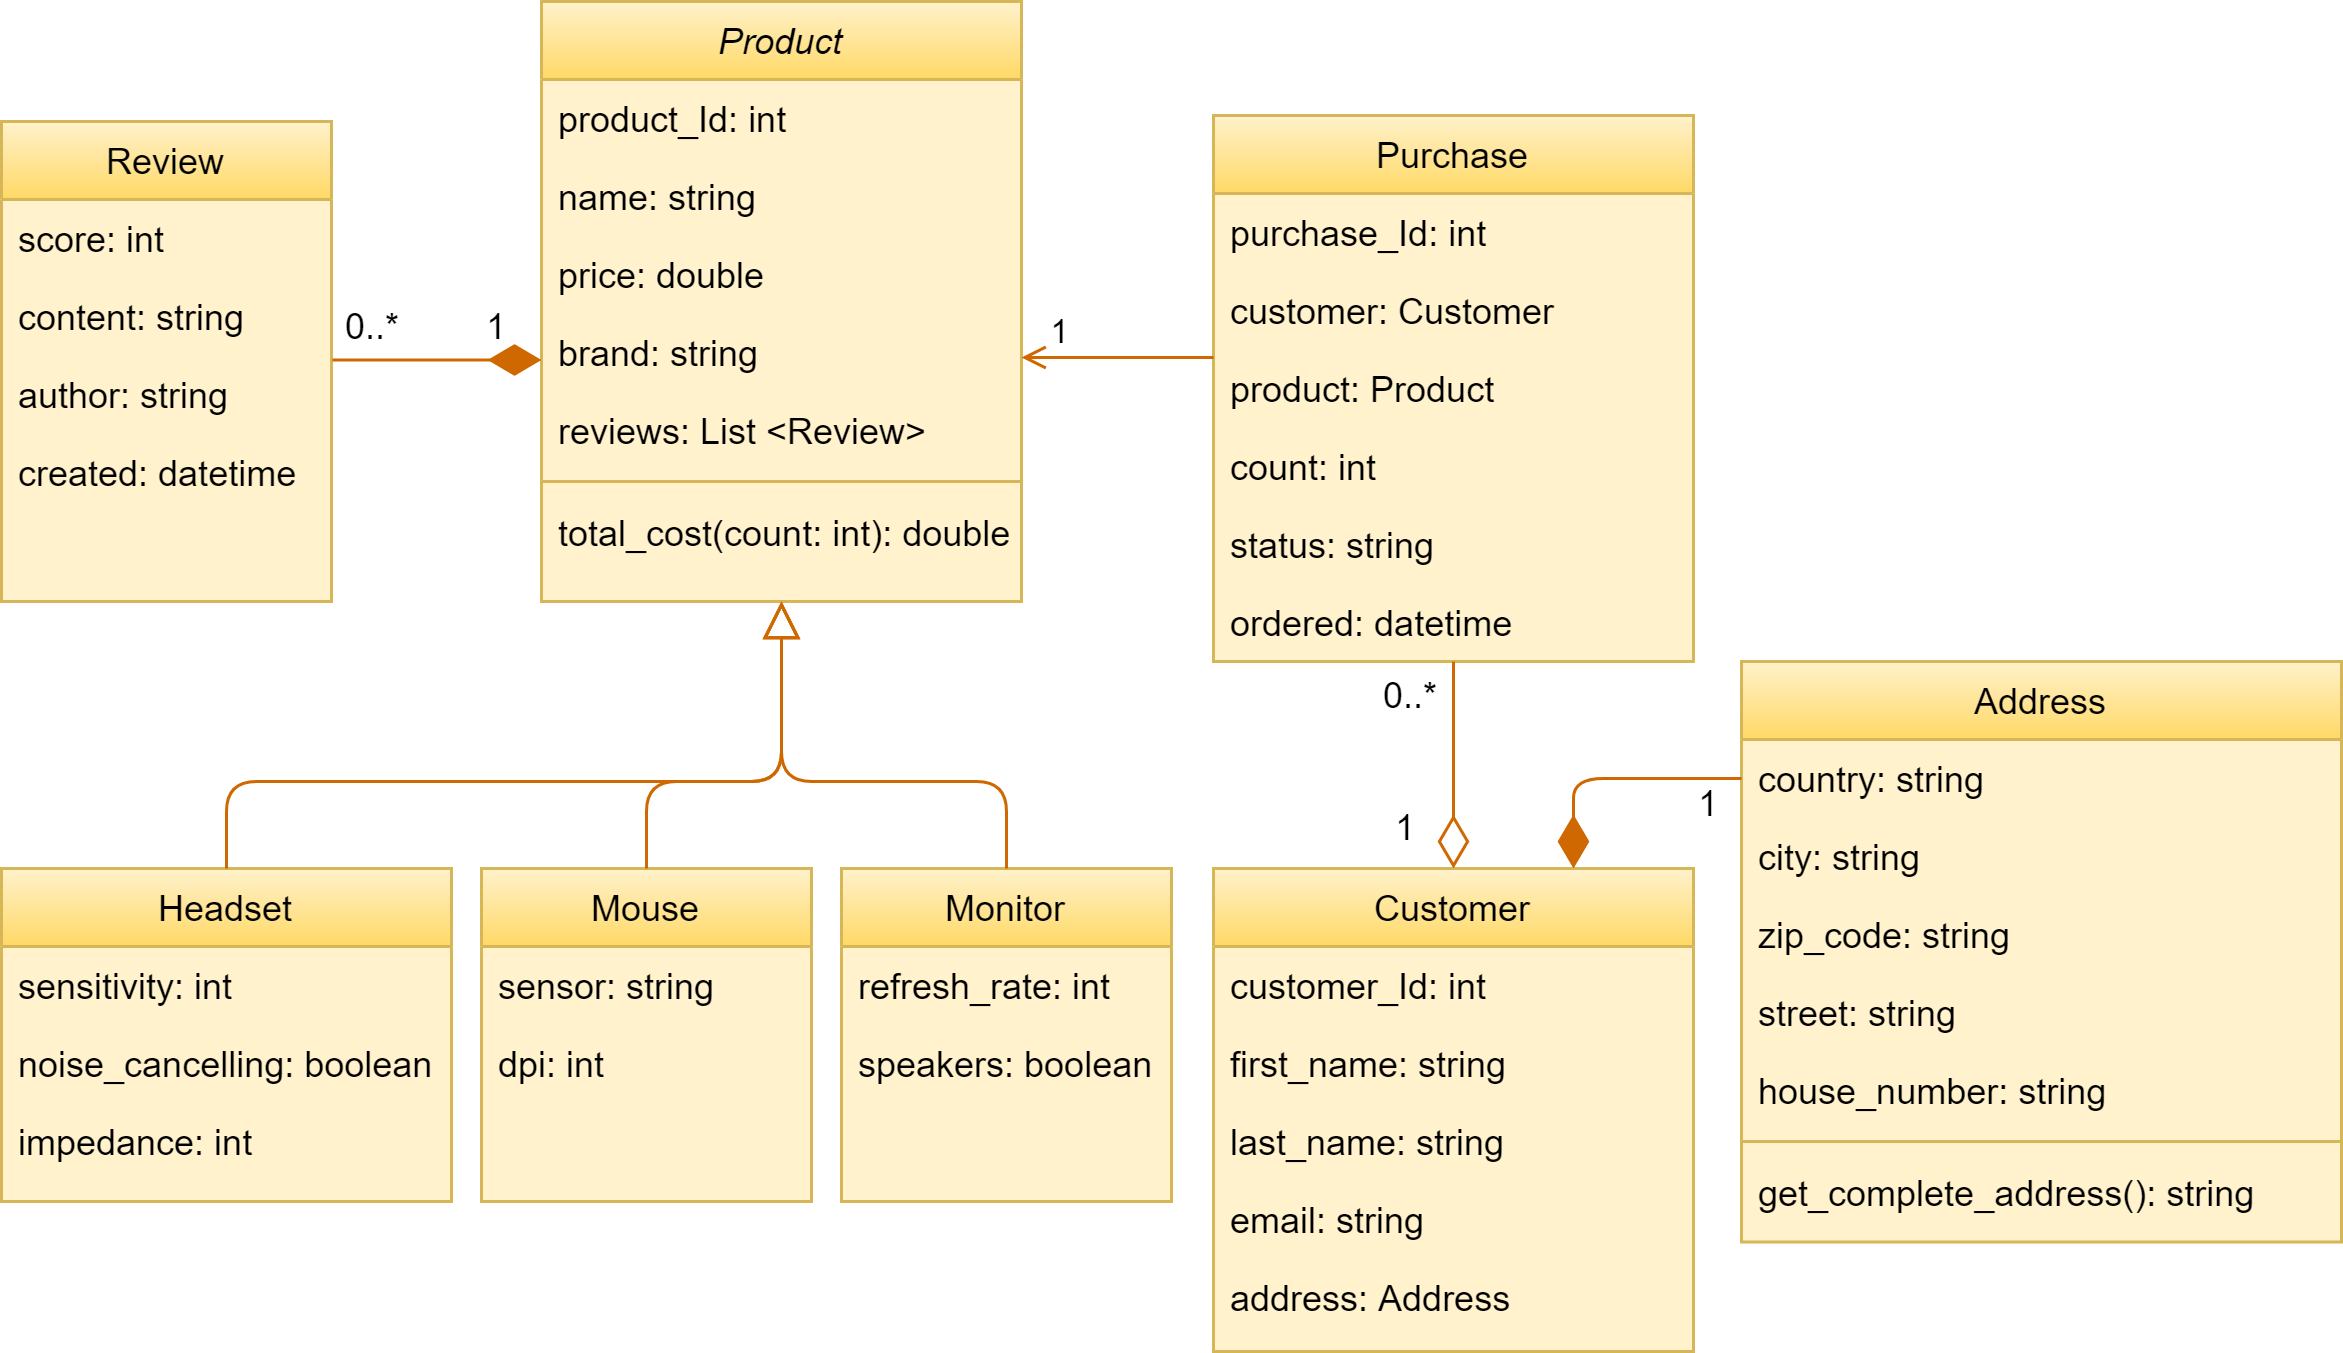
\includegraphics[height=8.6cm]{images/d1.png}
    \caption{Diagram klas modelowanej aplikacji.}
    \label{fig:diagram-klas}
\end{figure}

Głównym celem przyświecającym projektowaniu modelu było wykorzystanie różnych mechanizmów obiektowych, które będzie można odwzorować w ORSZBD. W zrealizowanym modelu występują następujące zjawiska obiektowe:
\begin{itemize}
\item Dziedziczenie - klasa \textit{Product} posiada trzy klasy potomne \textit{Monitor}, \textit{Headset} i \textit{Mouse}, z których każda posiada swoje własne unikalne pola. 
\item Zagnieżdżenie - klasa \textit{Address} jest zagnieżdżona w klasie \textit{Customer} i adres nigdy nie występuje jako niezależny obiekt.
\item Referencje - klasa \textit{Purchase} zawiera referencje (wskaźniki) do obiektów klas \textit{Customer} i \textit{Product}.
\item Typ kolekcji - klasa \textit{Product} zawiera w sobie listę obiektów klasy \textit{Review}.
\item Metody - klasa \textit{Address} zawiera metodę przygotowującą pełny adres w postaci jednego łańcucha tekstowego, a klasa \textit{Product} zawiera metodę obliczania kosztu wskazanej liczby produktów.
\end{itemize}

Można zauważyć, że metody klas zaproponowane w modelu są bardzo proste. Podczas projektowania modelu sugerowano się ograniczeniami analizowanych systemów, tak by nie wprowadzać metod, które są niemożliwe do zrealizowania. Żaden z systemów nie pozwala na trwałą modyfikację stanu obiektu podczas wywołania metody, ani na odwołanie do obiektów powiązanych przez referencję. Te ograniczenia uniemożliwiają tworzenie zaawansowanych metod, które bez problemu możnaby zrealizować w obiektowym języku programowania. Metody w ORSZBD mogą służyć w praktyce tylko do realizacji obliczeń lub wypisania informacji dla użytkownika, na podstawie pól obiektu i przekazanych parametrów.

\section{Podejście relacyjne}
\label{section:badania-relational}

Zasady projektowania struktury relacyjnej bazy danych zostały dobrze dopracowane przez wiele lat popularności tego rodzaju systemów. Schemat bazy został ręcznie zaprojektowany na podstawie rozpatrywanego diagramu klas z rysunku \ref{fig:diagram-klas}. Uzyskana struktura relacyjna przedstawiona jest na rysunku \ref{fig:diagram-rel}. Powstałe tabele w dużym stopniu odpowiadają modelowanym klasom, choć występuje kilka znaczących różnic.

\begin{figure}[!h]
    \centering
    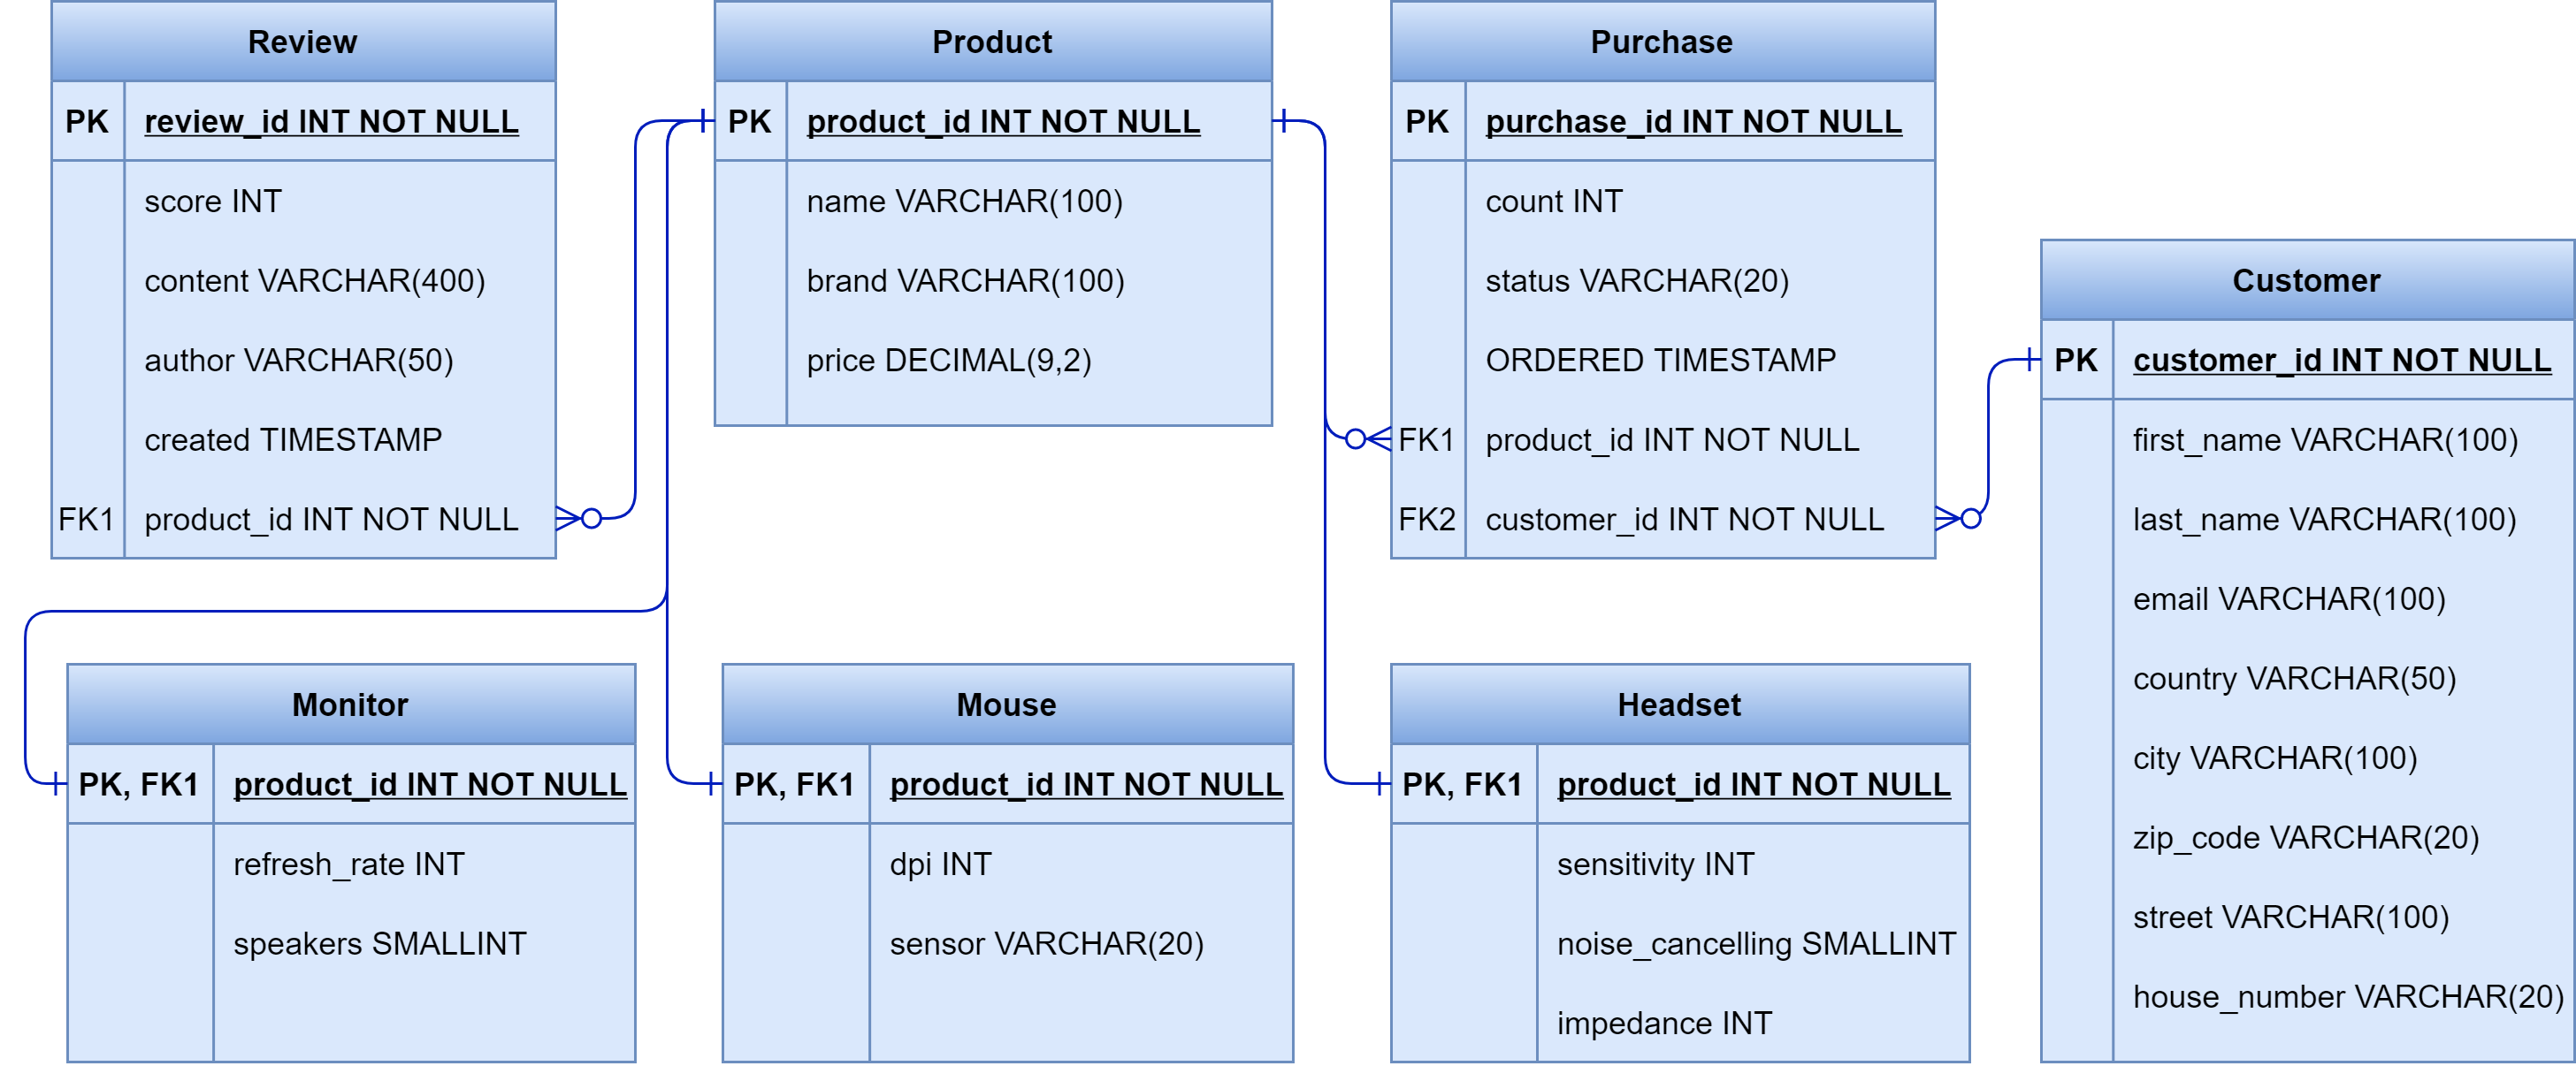
\includegraphics[width=15.1cm]{images/d2_v2.png}
    \caption{Diagram relacyjnej bazy danych.}
    \label{fig:diagram-rel}
\end{figure}

Związki pomiędzy danymi w różnych tabelach w świecie relacyjnym realizowane są za pomocą kluczy obcych. Warto zwrócić uwagę, że klucze obce modelujące powiązania przechowywane są zawsze w tabeli odpowiadającej większej krotności relacji (związek wiele-do-wielu wymaga utworzenia dodatkowej tabeli powiązań). Na przykładzie rozpatrywanej dziedziny, w tabeli recenzji w każdym wierszu przechowywana jest informacja, do którego produktu przynależy dana recenzja. Struktury obiektowe pozwalają na odwrócenie tej zależności i przechowanie listy obiektów wewnątrz innego obiektu. W takiej sytuacji, instancja produktu przechowywałaby informację o przynależących do niego recenzjach.

W przedstawionym rozwiązaniu nie ma odwzorowania osobnej tabeli dla adresu - pola klasy \textit{Address} zostały uwzględnione bezpośrednio w tabeli klientów. Alternatywą jest przechowanie adresów w osobnej tabeli i zapewnienie relacji z~klientem za pomocą klucza obcego - to rozwiązanie byłoby bardziej odpowiednie, gdyby adresy powtarzające się pomiędzy klientami traktowane były jako te same instancje danych.   

Model relacyjny nie posiada mechanizmów, które pozwoliłyby na dokładne odwzorowanie relacji dziedziczenia występującej w środowisku obiektowym. By umożliwić przechowywanie obiektów tworzących hierarchię dziedziczenia, powszechnie stosuje się trzy wzorce projektowe \cite{bib:fowler-patterns-of-enterprise-application-architecture}: 
\begin{itemize}
\item \textit{Single Table Inheritance} - spłaszczenie całej hierarchii dziedziczenia do jednej tabeli o wielu polach, które są wybiórczo wypełnione w różnych wierszach, zależnie od typu obiektu przechowywanego w danym wierszu.
\item \textit{Concrete Table Inheritance} - stworzenie po jednej tabeli dla każdej nieabstrakcyjnej klasy i uwzględnienie w nich pól abstrakcyjnych klas rodziców. To rozwiązanie uniemożliwia tworzenie relacji do abstrakcyjnego typu - klucze obce innych tabel mogą wskazywać jedynie na konkretne podtypy.
\item \textit{Class Table Inheritance} - stworzenie tabeli dla każdej klasy w hierarchii dziedziczenia i powiązanie ich wszystkich za pomocą jednego klucza.
\end{itemize}

W przedstawionym przykładzie zastosowano trzecią z opcji. Pole \textit{product\_id} występuje we wszystkich tabelach hierarchii produktów i pełni w nich rolę klucza głównego, a dodatkowo, w tabelach Monitor, Mouse i Headset pełni rolę klucza obcego, wskazującego na tabelę Product.

W modelu relacyjnym naturalnie nie uwzględniono metod, które występują wyłącznie w podejściu obiektowym. Zamiast nich użytkownik powinien stworzyć odpowiednie procedury albo powtórzyć logikę metod bezpośrednio w poleceniach SQL.

Jako że wiele SZBD nie wspiera typu \textit{Boolean}, we wszystkich omawianych rozwiązaniach wszystkie wystąpienia typu \textit{Boolean} reprezentowane są przez typ \textit{Smallint}, gdzie wartości 1 i 0 odpowiadają wartościom \textit{true} i \textit{
false}.

Bazując na diagramie bazy \ref{fig:diagram-rel} przygotowano skrypt SQL tworzący odpowiednie tabele. Skrypt jest uniwersalny i bez żadnych modyfikacji może być wykonany we wszystkich analizowanych systemach. Skrypt można znaleźć pod nazwą \textit{Relational-Structure.sql} w katalogu ``Scripts\textbackslash Structure'' na płycie dołączonej do pracy.

\section{Podejście obiektowo-relacyjne}

Tworząc strukturę bazy w systemach obiektowo-relacyjnych, starano się wiernie odwzorować strukturę klas z diagramu \ref{fig:diagram-klas}, uwzględniając wszystkie relacje dziedziczenia, referencji i agregacji. Mimo to, mechanizmy udostępniane przez poszczególne systemy są na tyle zróżnicowane, że występują znaczące różnice w powstałych strukturach, które zostaną omówione na podstawie komend tworzących poszczególne typy i tabele.

Kolejne podsekcje omawiają zaprojektowane struktury w oparciu o polecenia wykonywane w poszczególnych systemach. Skrypty zawierające komplet poleceń do utworzenia struktury obiektowo-relacyjnej w każdym systemie można znaleźć w katalogu ``Scripts\textbackslash Structure'' na płycie dołączonej do pracy.

\subsection{Oracle Database}

Odwzorowanie typów adresu i klienta jest dosyć proste i zrealizowane bardzo podobnie we wszystkich systemach. Fragment kodu \ref{listing:or-oracle-1} przedstawia komendy tworzące odpowiednie typy w bazie Oracle. Bez problemu można zawrzeć atrybut typu adresu wewnątrz typu klienta.

\begin{lstlisting}[style=SQL, caption={Definicja typów adresu i klienta w Oracle.}, label={listing:or-oracle-1}, captionpos=b]
CREATE TYPE Address_Type AS OBJECT (
  country       VARCHAR(50),
  city          VARCHAR(100),
  zip_code      VARCHAR(20),
  street        VARCHAR(100),
  house_number  VARCHAR(20),
  MEMBER FUNCTION get_complete_address RETURN VARCHAR
);
CREATE TYPE Customer_Type AS OBJECT (
  customer_id   INTEGER,
  first_name    VARCHAR(100),
  last_name     VARCHAR(100),
  email         VARCHAR(100),
  address       Address_Type
);
\end{lstlisting}

Korzystając ze stworzonego typu klienta można utworzyć tabelę klientów, korzystając z komendy \ref{listing:or-oracle-2}. Przy tworzeniu tabeli, atrybut \textit{customer\_id} wskazany jest jako klucz główny tabeli i jednocześnie wykorzystany jest jako identyfikator obiektu. Dzięki temu system nie będzie generował dodatkowych identyfikatorów, operując wartościami w kolumnie \textit{customer\_id} na potrzeby referencji i identyfikacji obiektów. 

\begin{lstlisting}[style=SQL, caption={Tworzenie tabeli klientów w Oracle.}, label={listing:or-oracle-2}, captionpos=b]
CREATE TABLE Customer OF Customer_Type (
	PRIMARY KEY (customer_id)
) OBJECT IDENTIFIER IS PRIMARY KEY;
\end{lstlisting}

W celu stworzenia typu produktu, konieczne jest wcześniejsze utworzenie typu recenzji, które przechowywane są jako lista wewnątrz każdego produktu. Oracle udostępnia świetnie przystosowany do tego mechanizm tabel zagnieżdżonych (ang. \textit{Nested Table}). Na fragmencie kodu \ref{listing:or-oracle-3} przedstawiono tworzenie typu recenzji oraz typu tabeli zagnieżdżonej, przechowującej recenzje. Alternatywą dla tego rozwiązania jest wykorzystanie kolekcji \lstinline{VARRAY}, która byłaby wskazana, gdyby maksymalna liczba recenzji była znana z góry. W przypadku nieograniczonej liczby elementów kolekcji bardziej uniwersalna jest tabela zagnieżdżona. 

\begin{lstlisting}[style=SQL, caption={Definicja typu recenzji i tabeli zagnieżdżonej recenzji w Oracle.}, label={listing:or-oracle-3}, captionpos=b]
CREATE TYPE Review_Type AS OBJECT (
  score         INTEGER,
  content       VARCHAR(400),
  author        VARCHAR(50),
  created       TIMESTAMP
);
CREATE TYPE Reviews_Type AS TABLE OF Review_Type;
\end{lstlisting}

Fragment kodu \ref{listing:or-oracle-4} przedstawia tworzenie typu produktu i tabeli produktów. Jako jeden z atrybutów wykorzystano typ tabeli zagnieżdżonej recenzji. W komendzie \lstinline{CREATE TABLE} wskazano nazwę tabeli, w której przechowywane mają być elementy zagnieżdżonej kolekcji. Podobnie jak dla tabeli klientów, tworząc tabelę produktów wskazano atrybut klucza głównego i nadano mu rolę identyfikatora obiektów. Definiując typ produktu wykorzystano frazę \lstinline{NOT FINAL}, by umożliwić tworzenie typów pochodnych od produktu. 

\begin{lstlisting}[style=SQL, caption={Definicja typu produktu i tworzenie tabeli produktów w Oracle.}, label={listing:or-oracle-4}, captionpos=b]
CREATE OR REPLACE TYPE Product_Type AS OBJECT (
  product_id    INTEGER,
  brand         VARCHAR(100),
  name          VARCHAR(100),
  price         DECIMAL(9,2),
  reviews       Reviews_Type,
  MEMBER FUNCTION total_cost (how_many IN INTEGER) RETURN DECIMAL
) NOT FINAL;

CREATE TABLE Product OF Product_Type (
	PRIMARY KEY (product_id)
) OBJECT IDENTIFIER IS PRIMARY KEY 
NESTED TABLE reviews STORE AS Reviews;
\end{lstlisting}

Bazując na typie produktu zdefiniowano dla niego trzy typy pochodne, jak przedstawiono na fragmencie kodu \ref{listing:or-oracle-5}. W rozwiązaniu Oracle, w kwestii dziedziczenia określa się tylko hierarchię typów i nie występuje dziedziczenie tabel, w~takim znaczeniu jak w innych omawianych systemach. Stworzenie hierarchii typów automatycznie umożliwia wstawianie dowolnego podtypu do tabeli zbudowanej w~oparciu o typ rodzica. W związku z tym nie ma potrzeby tworzenia osobnych tabel dla każdego podtypu.

\begin{lstlisting}[style=SQL, caption={Definicja podtypów produktu w Oracle.}, label={listing:or-oracle-5}, captionpos=b]
CREATE TYPE Monitor_Type UNDER Product_Type (
  refresh_rate  INTEGER,
  speakers      SMALLINT
);
CREATE TYPE Headset_Type UNDER Product_Type (
  sensitivity       INTEGER,
  impedance         INTEGER,
  noise_cancelling  SMALLINT
);
CREATE TYPE Mouse_Type UNDER Product_Type (
  dpi           INTEGER,
  sensor        VARCHAR(20)
);
\end{lstlisting}

Tworzenie typu reprezentującego zakup wymaga wykorzystania referencji, by wskazać powiązany produkt i klienta dokonującego zakupu. Odpowiednia komenda tworząca typ i tabelę zakupów przedstawiona jest na fragmencie kodu \ref{listing:or-oracle-6}. Podczas tworzenia tabeli określono zakres (ang. \textit{scope}) referencji, wskazując tabelę, w której przechowywane będą powiązane obiekty. Wskazanie zakresu jest opcjonalne, ale zwiększa wydajność dereferencji w zapytaniach. W przypadku tej tabeli również wskazano klucz główny i wykorzystano go jako identyfikator obiektów.

\begin{lstlisting}[style=SQL, caption={Definicja typu zakupu i tworzenie tabeli zakupów w Oracle.}, label={listing:or-oracle-6}, captionpos=b]
CREATE TYPE Purchase_Type AS OBJECT (
  purchase_id   INTEGER,
  customer      REF Customer_Type,
  product       REF Product_Type,
  count         INTEGER,
  status        VARCHAR(20),
  ordered       TIMESTAMP
);
CREATE TABLE Purchase OF Purchase_Type (
  product   SCOPE IS Product,
  customer  SCOPE IS Customer,
  PRIMARY   KEY (purchase_id)
) OBJECT IDENTIFIER IS PRIMARY KEY;
\end{lstlisting}

Na fragmentach kodu \ref{listing:or-oracle-1} i \ref{listing:or-oracle-4} w definicjach typów zawarte są specyfikacje metod. Dla każdego z tych typów konieczne jest określenie ciała typu, zawierającego treści metod, co przedstawia fragment kodu \ref{listing:or-oracle-7}. Warto zwrócić uwage, że określając typ zwracany przez metodę nie trzeba precyzować maksymalnego rozmiaru łańcucha znakowego \lstinline{VARCHAR} (linia 3) ani precyzji i skali typu \lstinline{DECIMAL} (linia 11).

\begin{lstlisting}[style=SQL, caption={Definicja ciał typów w Oracle.}, label={listing:or-oracle-7}, captionpos=b]
CREATE OR REPLACE TYPE BODY Address_Type AS 
  MEMBER FUNCTION get_complete_address 
  RETURN VARCHAR IS
  BEGIN
    RETURN street || ' ' || house_number || '\n' || zip_code || ' ' || city || ', ' || country;
  END;
END;

CREATE OR REPLACE TYPE BODY Product_Type AS 
  MEMBER FUNCTION total_cost (how_many IN INTEGER) 
  RETURN DECIMAL IS
  BEGIN
    RETURN how_many * price;
  END;
END;
\end{lstlisting}

Przykłady wstawiania danych do utworzonej struktury przedstawia fragment kodu \ref{listing:or-oracle-inserts-1}. Wstawianie obiektów różnych podtypów produktu wykonywane jest bezpośrednio na tabeli produktów. Oracle pilnuje unikalności klucza głównego również przy wstawianiu podtypów. Dodawanie wpisów do tabeli zakupów wymaga wykonania zagnieżdżonego zapytania \lstinline{SELECT} (linie 13-15), w celu uzyskania referencji do obiektów klienta i produktu.

\begin{lstlisting}[style=SQL, caption={Wstawianie danych do bazy Oracle.}, label={listing:or-oracle-inserts-1}, captionpos=b]
INSERT INTO Customer VALUES (1, 'Abel', 'Doe', 
  'abeldoes@mail.com', Address_Type('PL', 'Warsaw', 
  '44-300', 'Lubuska', '5/2'));

INSERT INTO Product VALUES (Monitor_Type(1, 'Aker', 
  'A1', 1200, Reviews_Type(), 60, 0));
INSERT INTO Product VALUES (Headset_Type(2, 'Fraction', 
  'F1', 1200, Reviews_Type(), 80, 32, 0));
INSERT INTO Product VALUES (Mouse_Type(3, 'Roar', 
  'R1', 500, Reviews_Type(), 1600, 'optical'));

INSERT INTO Purchase (
 SELECT Purchase_Type(1, REF(c), REF(p), 1, 'complete', '2021-08-27 15:23:54') 
 FROM Customer c, Product p 
 WHERE c.customer_id = 1 AND p.product_id = 5);
\end{lstlisting}

Dodawanie recenzji dla istniejącego produktu przedstawia fragment kodu \ref{listing:or-oracle-inserts-2}. Wykorzystano w tym celu operator \lstinline{MULTISET UNION ALL}, który łączy zawartość dwóch zbiorów - istniejącej listy recenzji i listy zawierającej jedną nową recenzję. Jest to najprostszy sposób na rozszerzenie zawartości zagnieżdżonej tabeli. 

\begin{lstlisting}[style=SQL, caption={Dodawanie nowej recenzji produktu w Oracle.}, label={listing:or-oracle-inserts-2}, captionpos=b]
UPDATE Product SET reviews = reviews MULTISET UNION ALL 
  Reviews_Type(Review_Type(5, 'Very good product!', 'anon01', '2021-08-27 18:20:15'))
WHERE product_id = 5;
\end{lstlisting}

\subsection{IBM Db2}

Tworzenie typów adresu i klienta w Db2 przedstawia fragment kodu \ref{listing:or-db2-1}. Podobnie jak w Oracle, w Db2 nie ma problemu z wykorzystaniem typu adresu jako jednego z atrybutów typu klienta. Wszystkie definicje typów w Db2 zakończone są wymaganą frazą \lstinline{MODE DB2SQL}.  

\begin{lstlisting}[style=SQL, caption={Definicja typów adresu i klienta w Db2.}, label={listing:or-db2-1}, captionpos=b]
CREATE TYPE Address_Type AS (
  country       VARCHAR(50),
  city          VARCHAR(100),
  zip_code      VARCHAR(20),
  street        VARCHAR(100),
  house_number  VARCHAR(20)
) MODE DB2SQL
METHOD get_complete_address () RETURNS VARCHAR(300) 
LANGUAGE SQL DETERMINISTIC;

CREATE TYPE Customer_Type AS (
  first_name    VARCHAR(100),
  last_name     VARCHAR(100),
  email         VARCHAR(100),
  address       Address_Type
) REF USING INTEGER MODE DB2SQL;
\end{lstlisting}

Na szczególną uwagę zasługuje brak atrybutu \lstinline{customer_id} w definicji typu klienta. W bazie Db2 tworzenie typowanej tabeli wymaga utworzenia kolumny identyfikatora obiektów, wykorzystywanej na potrzeby referencji. Kolumną identyfikatora nie może być żaden z atrybutów wchodzących w skład definicji typu. W rozpatrywanym modelu, typ klienta posiada identyfikator w postaci atrybutu \lstinline{customer_id}. By uniknąć przechowywania dwóch unikalnych identyfikatorów, usunięto wspomniany atrybut z definicji typu, ale dodano go jako kolumnę identyfikatora przy tworzeniu tabeli klientów, co widać na fragmencie kodu \ref{listing:or-db2-2}. Fraza \lstinline{REF USING} na fragmencie \ref{listing:or-db2-1} pozwala określić typ identyfikatora - wybrano typ \lstinline{INTEGER} by zachować spójność z pierwotnym modelem. To samo rozwiązanie wykorzystano przy tworzeniu pozostałych typów i tabel typowanych.

\begin{lstlisting}[style=SQL, caption={Tworzenie tabeli klientów w Db2.}, label={listing:or-db2-2}, captionpos=b]
CREATE TABLE Customer OF Customer_Type
(REF IS customer_id USER GENERATED);
\end{lstlisting}

System Db2 rozróżnia mechanizm dziedziczenia typów od dziedziczenia tabel. By odwzorować hierarchię produktów z rozpatrywanego modelu, należy najpierw utworzyć hierarchię typów, a następnie w analogiczny sposób stworzyć hierarchię tabel. Fragment kodu \ref{listing:or-db2-3} przedstawia tworzenie typu produktu i jego trzech podtypów, a fragment \ref{listing:or-db2-4} tworzenie hierarchii tabel.
 
\begin{lstlisting}[style=SQL, caption={Tworzenie typu produktu i jego podtypów w Db2.}, label={listing:or-db2-3}, captionpos=b]
CREATE TYPE Product_Type AS (
  brand     VARCHAR(100),
  name      VARCHAR(100),
  price     DECIMAL(9,2)
) NOT FINAL REF USING INTEGER MODE DB2SQL
METHOD total_cost(how_many INTEGER) 
RETURNS Decimal(12,2) LANGUAGE SQL DETERMINISTIC;

CREATE TYPE Monitor_Type UNDER Product_Type AS (
  refresh_rate  INTEGER,
  speakers      SMALLINT 
) MODE DB2SQL;

CREATE TYPE Headset_Type UNDER Product_Type AS (
  sensitivity       INTEGER,
  impedance         INTEGER,
  noise_cancelling  SMALLINT
) MODE DB2SQL;

CREATE TYPE Mouse_Type UNDER Product_Type AS (
  dpi           INTEGER,
  sensor        VARCHAR(20)
) MODE DB2SQL;
\end{lstlisting}

\vspace{0.2cm}

\begin{lstlisting}[style=SQL, caption={Tworzenie hierarchii tabel produktów w Db2.}, label={listing:or-db2-4}, captionpos=b]
CREATE TABLE Product OF Product_Type 
  (REF IS product_id USER GENERATED);
CREATE TABLE Monitor OF Monitor_Type UNDER Product 
  INHERIT SELECT PRIVILEGES;
CREATE TABLE Headset OF Headset_Type UNDER Product 
  INHERIT SELECT PRIVILEGES;
CREATE TABLE Mouse OF Mouse_Type UNDER Product 
  INHERIT SELECT PRIVILEGES;
\end{lstlisting}

\vspace{0.2cm}

Niestety w systemie Db2 nie ma możliwości wiernego zamodelowania relacji produktu i jego recenzji, tak by każdy produkt zawierał w ramach swojej struktury informację o liście recenzji. Choć dostępny jest typ kolekcji \lstinline{ARRAY}, ograniczony jest do przechowywania jedynie typów podstawowych - nie można wykorzystać go do przechowania obiektów typu użytkownika, ani typów referencji. 

\vspace{0.2cm}

W wyniku tego, jedyną pozostałą opcją jest odwrócenie relacji, tak by każda recenzja posiadała informację, do którego produktu jest przypisana. Rozwiązanie to jest bardzo zbliżone do rozwiązania relacyjnego - jedyną różnicą jest wykorzystanie referencji zamiast klucza obcego do wskazania produktu. Fragment kodu \ref{listing:or-db2-5} przedstawia tworzenie typu i tabeli recenzji. 

\begin{lstlisting}[style=SQL, caption={Tworzenie typu i tabeli recenzji w Db2.}, label={listing:or-db2-5}, captionpos=b]
CREATE TYPE Review_Type AS (
	score 		INTEGER,
	content 	VARCHAR(400),
	author		VARCHAR(50),
	created		TIMESTAMP,
	product 	REF(Product_Type)
) REF USING INTEGER MODE DB2SQL;

CREATE TABLE Review OF Review_Type (
	REF IS review_id USER GENERATED,
	product WITH OPTIONS SCOPE Product
);
\end{lstlisting}

Ostatnim tworzonym typem jest typ zakupu. Definicję typu i tworzenie typowanej tabeli przedstawia fragment kodu \ref{listing:or-db2-6}. Do wskazania klienta i produktu wykorzystano typ referencyjny (linie 2-3). Podczas tworzenia tabeli określono zakres referencji wskazując tabelę przechowującą referowane obiekty (linie 11-12).

\begin{lstlisting}[style=SQL, caption={Tworzenie typu i tabeli zakupów w Db2.}, label={listing:or-db2-6}, captionpos=b]
CREATE TYPE Purchase_Type AS (
  customer  REF(Customer_Type),
  product   REF(Product_Type),
  count     INTEGER,
  status    VARCHAR(20),
  ordered   TIMESTAMP
) REF USING INTEGER MODE DB2SQL;

CREATE TABLE Purchase OF Purchase_Type (
  REF IS purchase_id USER GENERATED,
  customer WITH OPTIONS SCOPE Customer,
  product  WITH OPTIONS SCOPE Product
);
\end{lstlisting}

Definicje typów na fragmentach kodu \ref{listing:or-db2-1} i \ref{listing:or-db2-3} zawierają specyfikacje metod. Ciała metod definiuje się za pomocą komendy \lstinline{CREATE METHOD}, co przedstawia fragment \ref{listing:or-db2-7}. Dostęp do pól instancji obiektu wewnątrz metod wymaga wykorzystania zmiennej \lstinline{SELF} i operatora dwóch kropek \textquotedbl..\textquotedbl. W odróżnieniu od rozwiązania Oracle, w przypadku Db2 w nagłówku metody konieczne jest dokładne określenie typu zwracanego, poprzez podanie maksymalnego rozmiaru łańcucha znakowego \lstinline{VARCHAR} oraz precyzji i skali typu \lstinline{DECIMAL}.

\begin{lstlisting}[style=SQL, caption={Tworzenie ciał metod w Db2.}, label={listing:or-db2-7}, captionpos=b]
CREATE METHOD get_complete_address () RETURNS VARCHAR (300) FOR Address_Type
RETURN SELF..street || ' ' || SELF..house_number || '\n' || SELF..zip_code || ' ' || SELF..city || ', ' || SELF..country;

CREATE METHOD total_cost(how_many INTEGER) RETURNS DECIMAL(12,2) FOR Product_Type
RETURN how_many * SELF..price;
\end{lstlisting}

Wstawianie danych klientów i produktów do utworzonej struktury bazy przedstawia fragment kodu \ref{listing:or-db2-inserts-1}. Jako pierwszy element we wszystkich poleceniach wstawiany jest typ referencyjny tworzony poprzez wywołanie odpowiedniej funkcji o~nazwie odpowiadającej typowi użytkownika.

W pierwszej komendzie widać charakterystyczne wykorzystanie bezargumentowego konstruktora typu adresu i łańcuchowe wywołanie automatycznie generowanych metod mutatorów w celu ustawienia wartości pól nowo utworzonego obiektu. Ponieważ adres przechowywany jest jako obiekt zagnieżdżony w typie klienta, dla tego obiektu nie ma potrzeby tworzenia typu referencyjnego.

Inaczej niż w bazie Oracle, obiekty podtypów produktu wstawiane są do odpowiadających im tabel uczestniczących w hierarchii dziedziczenia. Db2 pilnuje unikalności identyfikatora obiektów w ramach całej hierarchii tabel.

\begin{lstlisting}[style=SQL, caption={Wstawianie danych klientów i produktów do bazy Db2.}, label={listing:or-db2-inserts-1}, captionpos=b]
INSERT INTO Customer VALUES (Customer_Type(1), 'Abel', 
  'Doe', 'abeldoe@mail.com', Address_Type()
  ..country('PL')..city('Warsaw')..zip_code('44-300')
  ..street('Lubuska')..house_number('5/2'));

INSERT INTO Monitor VALUES (Monitor_Type(1), 'Aker', 
  'A1', 1200, 60, 0);
INSERT INTO Headset VALUES (Headset_Type(2), 'Fraction', 
  'F1', 1200, 80, 32, 0);
INSERT INTO Mouse VALUES (Mouse_Type(3), 'Roar', 
  'R1', 500, 1600, 'optical');
\end{lstlisting}

Fragment kodu \ref{listing:or-db2-inserts-2} pokazuje dwa sposoby wstawiania danych zakupów. Pierwsze polecenie jest bardzo podobne do swojego odpowiednika z bazy Oracle i zawiera zagnieżdżone zapytanie \lstinline{SELECT} pozwalające wyszukać identyfikatory (referencje) klienta i produktu. Druga wersja jest krótsza i może być wykorzystana gdy znane są wartości identyfikatorów. W przeciwieństwie do Oracle, Db2 pozwala na tworzenie pełnoprawnych referencji bez odnośników do obiektu, bazując na samej wartości identyfikatora.

\begin{lstlisting}[style=SQL, caption={Wstawianie danych zakupów do bazy Db2.}, label={listing:or-db2-inserts-2}, captionpos=b]
INSERT INTO Purchase
  SELECT Purchase_Type(1), c.customer_id, p.product_id, 
    1, 'complete', '2021-08-27 15:23:54'
  FROM Customer c, Product p 
  WHERE c.customer_id = Customer_Type(1) AND 
    p.product_id = Product_Type(5);

INSERT INTO Purchase VALUES (Purchase_Type(1), 
    Customer_Type(1), Product_Type(5), 
    1, 'complete', '2021-08-27 15:23:54');
\end{lstlisting}

Wstawianie recenzji dla istniejącego produktu przedstawiono na fragmencie kodu \ref{listing:or-db2-inserts-3}. Ta operacja jest prostsza niż w bazie Oracle, ponieważ recenzje nie są zagnieżdżone w produkcie, tylko przechowywane w osobnej tabeli.

\begin{lstlisting}[style=SQL, caption={Wstawianie recenzji do bazy Db2.}, label={listing:or-db2-inserts-3}, captionpos=b]
INSERT INTO Review VALUES (
  Review_Type(1), 5, 'Very good product!', 'anon01', 
  '2021-08-27 18:20:15', Product_Type(5)
);
\end{lstlisting}

\subsection{PostgreSQL}

Baza Postgres ma dosyć proste i ograniczone mechanizmy obiektowe, więc wiele spośród komend do generacji struktury bazy jest prostszych niż w pozostałych systemach. Komendy tworzące typy adresu są bardzo podobne do odpowiedników przedstawionych wcześniej. Przedstawia je fragment kodu \ref{listing:or-postgres-1}. W tym systemie również bardzo łatwo można zrealizować zagnieżdżenie adresu.

\begin{lstlisting}[style=SQL, caption={Tworzenie typów adresu i klienta w Postgres.}, label={listing:or-postgres-1}, captionpos=b]
CREATE TYPE Address_Type AS (
  country       VARCHAR(50),
  city          VARCHAR(100),
  zip_code      VARCHAR(20),
  street        VARCHAR(100),
  house_number  VARCHAR(20)
);
CREATE TYPE Customer_Type AS (
  customer_id   INTEGER,
  first_name    VARCHAR(100),
  last_name     VARCHAR(100),
  email         VARCHAR(100),
  address       Address_Type
);
\end{lstlisting}

Tworzenie tabeli klientów przedstawia fragment kodu \ref{listing:or-postgres-2}. Definiując tabelę wskazany został klucz główny. Tabele tworzone na podstawie typów nie posiadają specjalnego znaczenia w systemie Postgres, jak tabele typowane czy obiektowe w~Db2 i Oracle. Równoważny efekt do przedstawionego polecenia możnaby uzyskać wywołując komendę \lstinline{CREATE TABLE} bez podania typu użytkownika, a zamiast tego podając nazwy i typy wszystkich kolumn.

\begin{minipage}{\linewidth}
\begin{lstlisting}[style=SQL, caption={Tworzenie tabeli klientów w Postgres.}, label={listing:or-postgres-2}, captionpos=b]
CREATE TABLE Customer OF Customer_Type (
  PRIMARY KEY (customer_id)
);
\end{lstlisting}
\end{minipage}

Postgres umożliwia tworzenie kolekcji za pomocą typów tablic \lstinline{array}. W tablicach można przechowywać dowolne typy wartości, w tym również obiekty typów użytkownika, co nie jest możliwe w systemie Db2. Przy korzystaniu z \lstinline{array} możliwe jest nawet tworzenie tablic wielowymiarowych.

Fragment kodu \ref{listing:or-postgres-3} przedstawia tworzenie typu recenzji oraz typu produktu, w którym jednym z atrybutów jest tablica recenzji. Wykorzystanie tablicy nie wymaga definiowania dodatkowego typu, jak w bazie Oracle. Nie ma również potrzeby określenia maksymalnego rozmiaru tablicy - można ją swobodnie rozszerzać i dodawać elementy.

\begin{lstlisting}[style=SQL, caption={Tworzenie typu recenzji i produktu w Postgres.}, label={listing:or-postgres-3}, captionpos=b]
CREATE TYPE Review_Type AS (
  score         INTEGER,
  content       VARCHAR(400),
  author        VARCHAR(50),
  created       TIMESTAMP
);
CREATE TYPE Product_Type AS (
  product_id    INTEGER,
  brand         VARCHAR(100),
  name          VARCHAR(100),
  price         DECIMAL(9,2),
  reviews       Review_Type[]
);
\end{lstlisting}

Mechanizmy dziedziczenia w Postgres są stosunkowo ubogie w porównaniu do Oracle i Db2. Dostępne jest jedynie dziedziczenie tabel, podczas którego nie ma żadnej możliwości wskazania typu będącego wzorem dla struktury podtabeli. Tworzenie hierarchii tabel dla produktu i jego podtypów przedstawia fragment kodu \ref{listing:or-postgres-4}. W każdej definicji tabeli konieczne jest ponowne wskazanie klucza głównego - indeksy, klucze główne i obce oraz ograniczenia kolumn nie są dziedziczone w~Postgres. 

\begin{lstlisting}[style=SQL, caption={Tworzenie tabeli produktów i jej podtabel w Postgres.}, label={listing:or-postgres-4}, captionpos=b]
CREATE TABLE Product OF Product_Type (
  reviews   DEFAULT '{}',
  PRIMARY KEY (product_id)
);

CREATE TABLE Monitor (
  refresh_rate  INTEGER,
  speakers      SMALLINT,
  PRIMARY KEY (product_id)
) INHERITS (Product);

CREATE TABLE Headset (
  sensitivity       INTEGER,
  impedance         INTEGER,
  noise_cancelling  SMALLINT,
  PRIMARY KEY (product_id)
) INHERITS (Product);

CREATE TABLE Mouse (
  dpi       INTEGER,
  sensor    VARCHAR(20),
  PRIMARY KEY (product_id)
) INHERITS (Product);
\end{lstlisting}

Przy tworzeniu tabeli produktów dodatkowo wskazano wartość domyślną pustej tablicy dla atrybutu \lstinline{reviews} (linia 2), tak by tablica recenzji była zawsze zainicjalizowana, nawet jeśli recenzje nie zostaną wstawione wraz z produktem. Pozwala to na wygodne dodawanie elementów do tablicy bez konieczności sprawdzania czy tablica już istnieje.

Fragment kodu \ref{listing:or-postgres-5} przedstawia tworzenie typu i tabeli zakupów. W poleceniu tworzenia tabeli widać wadę Postgres w kwestii podejścia obiektowego - Postgres nie posiada żadnego mechanizmu referencji ani typów referencyjnych. Zamiast tego konieczne jest wykorzystanie kluczy obcych, dokładnie jak realizowane jest to w~rozwiązaniu relacyjnym.

\begin{lstlisting}[style=SQL, caption={Tworzenie typu i tabeli zakupów w Postgres.}, label={listing:or-postgres-5}, captionpos=b]
CREATE TYPE Purchase_Type AS (
  purchase_id   INTEGER,
  customer_id   INTEGER,
  product_id    INTEGER,
  count         INTEGER,
  status        VARCHAR(20),
  ordered       TIMESTAMP
);

CREATE TABLE Purchase OF Purchase_Type (
  PRIMARY KEY (purchase_id),
  FOREIGN KEY (customer_id) REFERENCES Customer
);
\end{lstlisting}

Podczas tworzenia tabeli zakupów celowo nie założono klucza obcego wskazującego na tabelę produktów. Wynika to z ogromnego problemu związanego ze stosowaniem dziedziczenia tabel - Postgres nie obsługuje propagacji i śledzenia klucza głównego pomiędzy tabelami w hierarchii dziedziczenia. Założenie klucza obcego na tabelę produktów pozwala tworzyć związki tylko do wartości przechowywanych bezpośrednio w tej tabeli, a nie w podtabelach. Jako że wszystkie instancje produktów należą do któregoś z podtypów i wstawiane są do odpowiedniej podtabeli, tworzenie takiego związku jest całkowicie nieprzydatne. 

\vspace{0.1cm}

Niestety obecnie nie ma rozwiązania dla tego problemu i bardzo ogranicza on przydatność dziedziczenia tabel w Postgres. Na potrzeby badań założono, że utrzymanie więzów integralności pomiędzy tabelą zakupów a tabelą produktów oraz zapewnienie unikalności kluczy głównych w całej hierarchii produktów pozostaje w gestii użytkownika bazy.

\vspace{0.1cm}

Postgres nie posiada mechanizmu metod powiązanych z typami. Zamiast tego możliwe jest tworzenie funkcji operujących na dowolnych typach, które w praktyce mogą skutecznie zastąpić metody. Definicje funkcji, odpowiadających metodom przygotowanym w Oracle i Db2, przedstawiono na fragmencie kodu \ref{listing:or-postgres-6}. Pierwszy parametr obu funkcji jest odpowiednikiem instancji obiektu, na której wywoływane są metody w pozostałych systemach. Podając parametry nie nadano im nazw - zamiast tego w treści metody odwołuje się do nich za pomocą numeru parametru. Symbol ``\$\$'' określa początek i koniec ciała metody.

\vspace{0.25cm}

\begin{lstlisting}[style=SQL, caption={Definicje funkcji w Postgres.}, label={listing:or-postgres-6}, captionpos=b]
CREATE OR REPLACE FUNCTION get_complete_address(
  Address_Type) RETURNS VARCHAR(300) AS 
  $$ SELECT ($1).street || ' ' || ($1).house_number || 
  '\n' || ($1).zip_code || ' ' || ($1).city || ', ' || 
  ($1).country $$
LANGUAGE sql;

CREATE OR REPLACE FUNCTION total_cost(
  Product_Type, integer) RETURNS DECIMAL AS 
  $$ SELECT ($1).price * $2 $$
LANGUAGE sql;
\end{lstlisting}

Wstawianie danych do tabel stworzonych w Postgres w dużej mierze realizowane jest tak samo jak dla standardowej struktury relacyjnej. Przykłady poleceń wstawiania danych przedstawia fragment kodu \ref{listing:or-postgres-inserts-1}. Wstawiając dane do tabeli klientów wykorzystano konstruktor wiersza \lstinline{ROW} do stworzenia obiektu adresu, którego typ jawnie wskazano za pomocą operatora ``\lstinline{::}''.

\vspace{0.1cm}

Dane produktów wstawiane są do odpowiednich podtabel w hierarchii dziedziczenia. Jak już wspomniano, Postgres nie posiada mechanizmów propagacji klucza głównego i nie pilnuje unikalności wartości klucza pomiędzy tabelami w hierarchii. Nic nie stoi na przeszkodzie by do każdej podtabeli wstawić wiersz o takiej samej wartości \lstinline{product_id}.

\vspace{0.1cm}

\begin{lstlisting}[style=SQL, caption={Wstawianie danych do bazy Postgres.}, label={listing:or-postgres-inserts-1}, captionpos=b]
INSERT INTO Customer VALUES (1, 'Abel', 'Doe', 
  'abeldoes@mail.com', ROW('PL', 'Warsaw', '44-300', 
  'Lubuska', '5/2')::Address_Type);

INSERT INTO Monitor VALUES 
  (1, 'Aker', 'A1', 1200, '{}', 60, 0);
INSERT INTO Headset VALUES 
  (2, 'Fraction', 'F1', 1200, '{}', 80, 32, 0);
INSERT INTO Mouse VALUES 
  (3, 'Roar', 'R1', 500, '{}', 1600, 'optical');

INSERT INTO Purchase VALUES 
  (1, 1, 5, 1, 'complete', '2021-08-27 15:23:54');
\end{lstlisting}

\vspace{0.1cm}

Dodawanie recenzji dla istniejącego produktu przedstawia fragment kodu \ref{listing:or-postgres-inserts-2}. W poleceniu wykorzystano wbudowaną funkcję \lstinline{array_append} (linia 2), która dodaje nowy element na ostatnią pozycję tablicy. 

\vspace{0.1cm}

\begin{lstlisting}[style=SQL, caption={Tworzenie typu i tabeli zakupów w Postgres.}, label={listing:or-postgres-inserts-2}, captionpos=b]
UPDATE Product SET reviews = 
  array_append(reviews, ROW(5, 'Very good product!',
  'anon01', '2021-08-27 18:20:15')::Review_Type)
WHERE product_id = 5;
\end{lstlisting}

\section{Generacja danych}

Do przeprowadzenia testów działania zaprojektowanych struktur, konieczne jest wprowadzenie do nich znaczącej liczby danych. W celu generacji danych stworzono aplikację w języku Java, z wykorzystaniem szkieletu aplikacyjnego Spring Boot, której zadaniem jest wygenerowanie skryptów SQL zawierających instrukcje wstawiające dane do wszystkich przygotowanych baz danych.
 
W aplikacji odwzorowano wszystkie klasy występujące w modelowanej domenie biznesowej, przedstawione na diagramie \ref{fig:diagram-klas}. Zachowano hierarchię dziedziczenia produktów, przynależność kolekcji recenzji do produktu oraz zagnieżdżenie adresu w klasie klienta. Dla każdej klasy modelu stworzono odpowiadającą klasę generatora, która tworzy instancje obiektów danego typu. Wartości pól obiektów dobierane są w sposób losowy według z góry określonych zasad.

Aplikacja posługuje się biblioteką \textit{lorem} \cite{bib:github-lorem}, która pozwala generować dowolną liczbę słów lub akapitów tekstu w stylu \textit{Lorem Ipsum}, co wykorzystano do tworzenia treści recenzji i nazw ulic. Oprócz tego \textit{lorem} pozwala generować losowe kody pocztowe, nazwy miast oraz państw. Miasta i państwa wybierane są ze skończonej listy predefiniowanych treści, dzięki czemu adresy w zbiorze danych zawierają powtarzające się wartości dla tych atrybutów.

Imiona i nazwiska klientów dobierane są losowo z listy wartości uzyskanej z~repozytorium \textit{NameDatabases} \cite{bib:github-names}, które zawiera zbiory imion i nazwisk dla różnych grup kulturowych. Email klienta tworzony jest poprzez złączenie jego imienia, nazwiska oraz końcówki ``mail.com''. Autorzy recenzji generowani są na podstawie tego samego zbioru, poprzez złączenie kilku pierwszych liter losowego imienia i~nazwiska. 

Producenci produktów dobierani są z autorskiej listy trzydziestu fikcyjnych nazw. Przygotowano także autorską listę trzydziestu słów składowych, z których budowane są nazwy produktów, poprzez połączenie od 1 do 3 losowo wybranych słów. Dla pewnej liczby produktów dodatkowo do nazwy dodawany jest dopisek ``Pro'' lub numer z zakresu od 2 do 6.

Unikalne identyfikatory wszystkich obiektów tworzone są poprzez inkrementację licznika obecnego w klasie generatora każdego typu. Wszystkie wartości liczbowe generowane są losowo w ramach  określonych przedziałów. Daty i godziny stworzenia recenzji oraz dokonania zakupu losowane są z zakresu od 01.01.2015 do 05.09.2021. Wartości tekstowe dla sensora myszy oraz statusu zakupu wybierane są ze zbioru kilku predefiniowanych wartości.

Efektem działania aplikacji jest powstanie czterech plików tekstowych zawierających polecenia SQL. Trzy z nich zawierają komendy dostosowane do struktur obiektowo-relacyjnych w systemach Oracle, Db2 i Postgres. Czwarty plik zawiera uniwersalne polecenia dla struktury relacyjnej, które są poprawne dla każdego systemu. Większość poleceń w pliku to polecenia \lstinline{INSERT}, jedynie dla struktur obiektowo-relacyjnych w Oracle i Postgres występują polecenia \lstinline{UPDATE} dla wstawiania recenzji do zagnieżdżonych kolekcji. Recenzje nie są wstawiane razem z~produktem, tylko w osobnych, niezależnych poleceniach, by symulować zachowanie prawdziwego systemu, w którym recenzje dodawane byłyby stopniowo dla istniejących produktów. Wszystkie wygenerowane skrypty można znaleźć na płycie dołączonej do pracy w katalogu ``Scripts\textbackslash Data''.

Zbiór danych wygenerowany na potrzeby pracy zawiera 100 000 klientów, 10~000 każdego typu produktów, 300 000 zakupów i 200 000 recenzji. Wstawianie tak dużej ilości danych do bazy jest stosunkowo czasochłonne. Czasy wykonania skryptów wstawiających dane dla każdego systemu w obu strukturach bazy przedstawia tabela \ref{table:czas-wstawiania-danych}. Najdłuższe czasy zaobserwowano dla systemu Db2, a najkrótsze dla PostgreSQL. We wszystkich systemach wstawianie danych dla struktury obiektowo-relacyjnej trwało dłużej niż dla struktury relacyjnej.

\renewcommand\cellgape{\Gape[4pt]}

\begin{table}[h!]
\centering
\caption{Czasy wstawiania danych do stworzonych struktur.}
\label{table:czas-wstawiania-danych}
\begin{tabular}{ | m{4cm} || >{\centering}m{2.8cm} | >{\centering}m{2.8cm} | >{\centering\arraybackslash}m{2.8cm} |}
 \hline 
 \makecell{Struktura} & \thead{Oracle} & \thead{Db2} & \thead{Postgres} \\ 
 \hline \hline
 Obiektowo-relacyjna  & 72 min & 130 min & 54 min \\  
 \hline
 Relacyjna            & 60 min & 122 min & 49 min \\  
 \hline
\end{tabular}
\end{table}

\section{Zapytania testowe}

Dla wszystkich utworzonych struktur obiektowo-relacyjnych przygotowano szereg zapytań realizujących przykładowe operacje biznesowe. Przygotowano również zapytania dla struktur relacyjnych, utworzonych w każdym systemie zgodnie z~modelem przedstawionym w sekcji \ref{section:badania-relational} \nameref{section:badania-relational}. Głównym celem przedstawionych zapytań jest prezentacja możliwości oraz ograniczeń występujących podczas pracy ze strukturami obiektowo-relacyjnymi w analizowanych systemach. Celowo wybrano zróżnicowane zagadnienia, tak aby pokazać szeroki zakres problemów i sposobów ich rozwiązania.

Wszystkie przygotowane zapytania wykonano pięciokrotnie na tym samym zbiorze danych i zmierzono czas ich realizacji. Dla każdego zapytania przedstawiono najdłuższy i najkrótszy czas wykonania, wartość średnią oraz odchylenie standardowe. Porównując uzyskane wyniki, należy jednak pamiętać o dużych różnicach w strukturach zaimplementowanych w poszczególnych systemach. W rozwiązaniach nie wprowadzono także żadnych indeksów, które mogłyby znacząco wpłynąć na prędkość realizacji zapytań.

W procesie testowania, w każdym systemie stworzono strukturę obiektowo-relacyjną, wstawiono do niej zbiór danych i wykonano wszystkie zaplanowane zapytania. Następnie całkowicie wyczyszczono bazę i powtórzono proces dla struktury relacyjnej, tak by w bazie przechowywany był zawsze tylko jeden zestaw danych.

\subsection{Zapytanie 1 - Średnia ocena wybranego produktu}

Cel zapytania: \textit{Obliczyć średnią ocenę wybranego produktu na podstawie wszystkich jego recenzji}. 

Na potrzeby tego zagadnienia zakłada się, że znany jest identyfikator produktu, który został wyszukany wcześniej, w oparciu o nazwę, producenta lub inne cechy. Ta sama zasada dotyczy wszystkich zapytań, które odnoszą się do wybranego produktu lub klienta.

Fragment kodu \ref{listing:zapytanie-1-rel} przedstawia realizację operacji w podejściu relacyjnym. Recenzje przechowywane są w osobnej tabeli i posiadają klucz obcy wskazujący na produkt, który wykorzystano do wyboru recenzji związanych z konkretnym produktem. 

\begin{lstlisting}[style=SQL, caption={Zapytanie pierwsze w podejściu relacyjnym.}, label={listing:zapytanie-1-rel}, captionpos=b]
SELECT  AVG(score)
FROM    Review
WHERE   product_id = 15000;
\end{lstlisting}

Treść zapytania dla bazy Oracle przedstawiona jest na fragmencie \ref{listing:zapytanie-1-oracle}. W tej strukturze lista recenzji przechowywana jest jako tabela zagnieżdżona wewnątrz typu produktu. By uzyskać dostęp do kolekcji wykorzystano operator \lstinline{TABLE}, który wydobywa zagnieżdżone dane do zmiennej i pozwala z nich korzystać jak ze standardowej tabeli.

\begin{lstlisting}[style=SQL, caption={Zapytanie pierwsze w Oracle.}, label={listing:zapytanie-1-oracle}, captionpos=b]
SELECT AVG(r.score)
FROM   product p, TABLE(p.reviews) r
WHERE  product_id = 15000;
\end{lstlisting}

\vspace{0.1cm}

Realizacja zapytania w Db2 przedstawiona jest na fragmencie \ref{listing:zapytanie-1-db2}. Ponieważ recenzje w Db2 przechowywane są w osobnej tabeli, treść zapytania jest bardzo podobna do rozwiązania relacyjnego. Zamiast klucza głównego wybór recenzji wykonuje się przyrównując kolumnę referencji do instancji typu referencyjnego. By zwrócić wynik w postaci ułamka, w pierwszej linii zapytania dodatkowo wykonano rzutowanie oceny na typ \lstinline{DECIMAL} - bez tego zwrócony byłby typ całkowity, bo operacja \lstinline{AVG} w Db2 domyślnie zwraca taki sam typ jak typ uśrednianych elementów.

\vspace{0.1cm}

\begin{lstlisting}[style=SQL, caption={Zapytanie pierwsze w Db2.}, label={listing:zapytanie-1-db2}, captionpos=b]
SELECT  AVG(CAST(score AS DECIMAL(4,2)))
FROM    Review
WHERE   product = Product_Type(15000);
\end{lstlisting}

Treść zapytania w Postgres przedstawia fragment \ref{listing:zapytanie-1-postgres}. W tej strukturze recenzje przechowywane są jako tablica w obiekcie produktu. By wydobyć elementy listy recenzji wykorzystano operator \lstinline{UNNEST}, który tworzy zbiór wierszy na podstawie kolekcji. Wyliczenie średniej odbywa się w zagnieżdżonym zapytaniu \lstinline{SELECT}.

\begin{lstlisting}[style=SQL, caption={Zapytanie pierwsze w Postgres.}, label={listing:zapytanie-1-postgres}, captionpos=b]
SELECT (SELECT AVG(r.score) FROM UNNEST(reviews) r)
FROM  product
WHERE product_id = 15000;
\end{lstlisting}

Czasy wykonania zapytań we wszystkich systemach przedstawia tabela \ref{table:zapytanie-1-results}. Na uwagę zasługuje szczególnie niski czas uzyskany w Oracle w strukturze obiektowo-relacyjnej, gdzie średni czas to 7,6 ms. Tak dobre wyniki są prawdopodobnie efektem wykorzystania tabeli zagnieżdżonej do przechowywania recenzji. Dla Db2 czasy realizacji są bardzo zbliżone w obu strukturach. W Postgres uzyskano około 25\% lepsze wyniki dla struktury obiektowo-relacyjnej.

\renewcommand\cellgape{\Gape[4pt]}

\begin{table}[h!]
\centering
\caption{Czasy wykonania pierwszego zapytania.}
\label{table:zapytanie-1-results}
\begin{tabular}{ | >{\centering}m{3.0cm} | >{\centering}m{2.0cm} | >{\centering}m{2.0cm} | >{\centering}m{2.0cm} | >{\centering\arraybackslash}m{2.0cm} |}
 \hline 
 \multicolumn{5}{|c|}{\thead{Struktura relacyjna}} \\
 \hline 
 \thead{System} & \thead{Średnia} & \thead{Min} & \thead{Max} & \thead{\bm{$ \sigma $}} \\ 
 \hline 
 Oracle     & 26,8 ms & 21 ms & 46 ms & 10,76 ms \\  
 \hline
 Db2        & 35,6 ms & 25 ms & 74 ms & 21,49 ms \\  
 \hline
 Postgres   & 61,8 ms & 58 ms & 68 ms & 4,49 ms \\  
 \hline \hline
 \multicolumn{5}{|c|}{\thead{Struktura obiektowo-relacyjna}} \\
 \hline 
 \thead{System} & \thead{Średnia} & \thead{Min} & \thead{Max} & \thead{\bm{$ \sigma $}} \\ 
 \hline
 Oracle     & 7,6 ms & 5 ms & 12 ms & 2,70 ms \\  
 \hline
 Db2        & 36 ms & 30 ms & 55 ms & 10,70 ms \\  
 \hline
 Postgres   & 45,8 ms & 42 ms & 52 ms & 4,15 ms \\  
 \hline
\end{tabular}
\end{table}

\subsection{Zapytanie 2 - Negatywne recenzje produktów producenta}

Cel zapytania: \textit{Wypisać szczegóły wszystkich recenzji z oceną 1 utworzonych dla produktów wybranego producenta oraz nazwę i cenę powiązanych produktów}.

\vspace{0.1cm}

Realizacja zagadnienia w podejściu obiektowym przedstawiona jest na fragmencie kodu \ref{listing:zapytanie-2-rel}. Za pomocą identyfikatora \lstinline{product_id} łączone są tabele recenzji i~produktów. Wykonane jest filtrowanie wyników po nazwie producenta oraz wyniku recenzji i zwrócone są wymagane atrybuty.

\vspace{0.1cm}

\begin{lstlisting}[style=SQL, caption={Zapytanie drugie w podejściu relacyjnym.}, label={listing:zapytanie-2-rel}, captionpos=b]
SELECT p.name, p.price, r.*
FROM  Review r JOIN Product p 
ON    p.product_id = r.product_id
WHERE p.brand = 'Vester' AND r.score = 1;
\end{lstlisting}

Zapytanie dla Oracle przedstawia fragment kodu \ref{listing:zapytanie-2-oracle}. Dostęp do elementów zagnieżdżonej kolekcji recenzji uzyskuje się za pomocą funkcji \lstinline{TABLE}, po czym kolekcja wykorzystana jest tak jak zwykła tabela i reszta zapytania wygląda prawie identycznie do wersji relacyjnej. 

\vspace{0.1cm}

\begin{lstlisting}[style=SQL, caption={Zapytanie drugie w Oracle.}, label={listing:zapytanie-2-oracle}, captionpos=b]
SELECT p.name, p.price, r.*
FROM   product p, TABLE(p.reviews) r
WHERE  brand = 'Vester' AND r.score = 1;
\end{lstlisting}

Wersję zapytania dla Db2 przedstawia fragment \ref{listing:zapytanie-2-db2}. W tej strukturze recenzje przechowywane są w osobnej tabeli, a relację recenzji i produktu realizuje kolumna przechowująca referencję. Za pomocą operatora dereferencji ``->'' możliwy jest dostęp do atrybutów powiązanego produktu.

\vspace{0.1cm}

\begin{lstlisting}[style=SQL, caption={Zapytanie drugie w Db2.}, label={listing:zapytanie-2-db2}, captionpos=b]
SELECT  product->name, product->price, r.*
FROM    Review r
WHERE   product->brand = 'Vester' AND r.score = 1;
\end{lstlisting}

Realizację zapytania w Postgres przedstawia fragment kodu \ref{listing:zapytanie-2-postgres}. Treść zapytania jest bardzo podobna do rozwiązania w Oracle, jednak tutaj zamiast funkcji \lstinline{TABLE} wykorzystano funkcję \lstinline{UNNEST} do wydobycia zagnieżdżonej tablicy recencji. Pozostała część zapytania jest identyczna jak w Oracle.

\begin{lstlisting}[style=SQL, caption={Zapytanie drugie w Postgres.}, label={listing:zapytanie-2-postgres}, captionpos=b]
SELECT p.name, p.price, r.*
FROM   product p, UNNEST(p.reviews) r
WHERE  brand = 'Vester' AND r.score = 1;
\end{lstlisting}

Czasy wykonania zapytań we wszystkich systemach przedstawia tabela \ref{table:zapytanie-2-results}. Podobnie jak dla pierwszego zapytania, widoczny jest szybki czas wykonania dla struktury obiektowo-relacyjnej w Oracle, jednak w tym przypadku równie dobre rezultaty widać dla struktury relacyjnej w Oracle i Db2. Czas realizacji dla struktury obiektowo-relacyjnej w Db2 jest około dwa razy dłuższy niż dla struktury relacyjnej. Można po tym wnioskować, wykorzystanie dereferencji skutkuje gorszą wydajnością niż przy relacyjnym łączeniu tabel. Czasy wykonania w Postgres dla obu struktur są znacznie wyższe niż w pozostałych systemach.

\begin{table}[h!]
\centering
\caption{Czasy wykonania drugiego zapytania.}
\label{table:zapytanie-2-results}
\begin{tabular}{ | >{\centering}m{3.0cm} | >{\centering}m{2.0cm} | >{\centering}m{2.0cm} | >{\centering}m{2.0cm} | >{\centering\arraybackslash}m{2.0cm} |}
 \hline 
 \multicolumn{5}{|c|}{\thead{Struktura relacyjna}} \\
 \hline 
 \thead{System} & \thead{Średnia} & \thead{Min} & \thead{Max} & \thead{\bm{$ \sigma $}} \\ 
 \hline 
 Oracle     & 6 ms & 5 ms & 7 ms & 0,71 ms \\  
 \hline
 Db2        & 8,2 ms & 6 ms & 14 ms & 3,27 ms \\  
 \hline
 Postgres   & 98,6 ms & 94 ms & 105 ms & 5,13 ms \\  
 \hline \hline
 \multicolumn{5}{|c|}{\thead{Struktura obiektowo-relacyjna}} \\
 \hline 
 \thead{System} & \thead{Średnia} & \thead{Min} & \thead{Max} & \thead{\bm{$ \sigma $}} \\ 
 \hline
 Oracle     & 7,2 ms & 6 ms & 9 ms & 1,10 ms \\  
 \hline
 Db2        & 16,6 ms & 15 ms & 21 ms & 2,51 ms \\  
 \hline
 Postgres   & 84 ms & 78 ms & 93 ms & 5,66 ms \\  
 \hline
\end{tabular}
\end{table}

\subsection{Zapytanie 3 - Suma wydatków klienta w wybranym okresie czasu}

Cel zapytania: \textit{Obliczyć sumę kosztów wszystkich zakupów wykonanych przez wybranego klienta w okresie czasu pomiędzy dwoma datami}.

Wersja zapytania w podejściu relacyjnym przedstawiona jest na fragmencie kodu \ref{listing:zapytanie-3-rel}. Za pomocą wartości identyfikatorów łączone są trzy tabele: produktów, klientów oraz zakupów. We frazie \lstinline{WHERE} wskazany jest klient oraz zakres czasu zakupów. Ceny produktów mnożone są przez liczbę produktów zamówionych w~ramach pojedynczego zakupu, a suma uzyskanych wartości stanowi wynik zapytania. 

\begin{lstlisting}[style=SQL, caption={Zapytanie trzecie w podejściu relacyjnym.}, label={listing:zapytanie-3-rel}, captionpos=b]
SELECT SUM(price * count)
FROM  Customer, Purchase, Product
WHERE Customer.customer_id = 25000
AND ordered >= '2018-01-01' AND ordered <= '2021-08-30'
AND Customer.customer_id = Purchase.customer_id
AND Product.product_id = Purchase.product_id;
\end{lstlisting}

Rozwiązanie zagadnienia w Oracle przedstawia fragment \ref{listing:zapytanie-3-oracle}. Tutaj możliwe jest wykorzystanie referencji, co upraszcza składnię zapytania. Z tabeli zakupów za pomocą referencji można odnieść się do obiektów klienta i produktu, dzięki czemu nie ma potrzeby wskazywania połączeń pomiędzy tabelami. W celu obliczenia kosztów poszczególnych zakupów wykorzystano metodę \lstinline{total_cost}, która wykonuje mnożenie kosztu produktu i liczby zakupionych elementów.

\begin{lstlisting}[style=SQL, caption={Zapytanie trzecie w Oracle.}, label={listing:zapytanie-3-oracle}, captionpos=b]
SELECT SUM(p.product.total_cost(count))
FROM  Purchase p
WHERE p.customer.customer_id = 25000
AND ordered >= '2018-01-01' AND ordered <= '2021-08-30';
\end{lstlisting}

Zapytanie w Db2 przedstawia fragment \ref{listing:zapytanie-3-db2}. Format zapytania jest bardzo podobny do wersji Oracle. Tutaj również wykorzystano referencję, by odnieść się do klienta i produktu. W celu wyboru klienta nałożono warunek porównujący referencję ze skonstruowanym typem referencyjnym. Podobnie jak w rozwiązaniu dla Oracle wykorzystano metodę \lstinline{total_cost}, wywołując ją za pomocą charakterystycznego operatora dereferencji ``->''.

\begin{lstlisting}[style=SQL, caption={Zapytanie trzecie w Db2.}, label={listing:zapytanie-3-db2}, captionpos=b]
SELECT SUM(p.product->total_cost(p.count))
FROM   Purchase p
WHERE  p.customer = Customer_Type(25000)
AND ordered >= '2018-01-01' AND ordered <= '2021-08-30';
\end{lstlisting}

Treść zapytania w systemie Postgres przedstawia fragment \ref{listing:zapytanie-3-postgres}. W tym systemie nie występują referencje, więc zapytanie jest bardzo zbliżone do rozwiązania relacyjnego i jedyną różnicą jest wykorzystanie funkcji \lstinline{total_cost}. Ponieważ Postgres nie obsługuje metod, operacja ta stworzona jest jako funkcja, do której przekazuje się produkt i liczbę zakupionych elementów. 

\begin{minipage}{\linewidth}
\begin{lstlisting}[style=SQL, caption={Zapytanie trzecie w Postgres}, label={listing:zapytanie-3-postgres}, captionpos=b]
SELECT SUM(total_cost(Product, count))
FROM Customer, Purchase, Product
WHERE Customer.customer_id = 25000
AND ordered >= '2018-01-01' AND ordered <= '2021-08-30'
AND Customer.customer_id = Purchase.customer_id
AND Product.product_id = Purchase.product_id;
\end{lstlisting}
\end{minipage}

Czasy wykonania zapytań we wszystkich systemach przedstawia tabela \ref{table:zapytanie-3-results}. Wyniki w Postgres dla obu struktur są niemal identyczne, ponieważ w tym systemie fragment bazy istotny dla realizowanego zagadnienia jest taki sam w obu podejściach. Wykorzystanie funkcji zamiast bezpośredniego łączenia pól w zapytaniu nie ma znaczącego wpływu na czas realizacji zapytania. Dla struktury obiektowo-relacyjnej Db2 uzyskało bardzo podobny wynik co Postgres, a Oracle uzyskało czasy około 55\% krótsze. Różnica w wynikach jest zaskakująca, ponieważ treść zapytania dla tej struktury jest bardzo podobna w Db2 i Oracle. Najlepsze wyniki uzyskano w strukturze relacyjnej w Db2 i Oracle - w obu systemach średni czas wykonania zapytania wyniósł około 17 ms. W przypadku Oracle można zaobserwować wysokie odchylenie standardowe i dużą różnicę pomiędzy minimalnym i~maksymalnym czasem. Najdłuższy czas 56 ms uzyskano przy pierwszym wykonaniu zapytania; kolejne czasy wykonania były dużo krótsze, ponieważ system skutecznie wykorzystał mechanizm pamięci podręcznej (ang. \textit{cache}) w celu szybszej realizacji zapytania.

\begin{table}[h!]
\centering
\caption{Czasy wykonania trzeciego zapytania.}
\label{table:zapytanie-3-results}
\begin{tabular}{ | >{\centering}m{3.0cm} | >{\centering}m{2.0cm} | >{\centering}m{2.0cm} | >{\centering}m{2.0cm} | >{\centering\arraybackslash}m{2.0cm} |}
 \hline 
 \multicolumn{5}{|c|}{\thead{Struktura relacyjna}} \\
 \hline 
 \thead{System} & \thead{Średnia} & \thead{Min} & \thead{Max} & \thead{\bm{$ \sigma $}} \\ 
 \hline 
 Oracle     & 17,4 ms & 7 ms & 56 ms & 21,59 ms \\  
 \hline
 Db2        & 16,4 ms & 16 ms & 17 ms & 0,55 ms \\  
 \hline
 Postgres   & 69,2 ms & 57 ms & 103 ms & 19,29 ms \\  
 \hline \hline
 \multicolumn{5}{|c|}{\thead{Struktura obiektowo-relacyjna}} \\
 \hline 
 \thead{System} & \thead{Średnia} & \thead{Min} & \thead{Max} & \thead{\bm{$ \sigma $}} \\ 
 \hline
 Oracle     & 30,8 ms & 28 ms & 37 ms & 3,63 ms \\  
 \hline
 Db2        & 69,6 ms & 61 ms & 76 ms & 6,15 ms \\  
 \hline
 Postgres   & 68,8 ms & 62 ms & 88 ms & 10,80 ms \\  
 \hline
\end{tabular}
\end{table}

\subsection{Zapytanie 4 - Największa liczba recenzji dla pojedynczego produktu}

Cel zapytania: \textit{Znaleźć maksymalną liczbę recenzji utworzonych dla pojedynczego produktu}.

Relacyjna wersja zapytania przedstawiona jest na fragmencie kodu \ref{listing:zapytanie-4-rel}. Jednocześnie jest to także rozwiązanie dla struktury obiektowo-relacyjnej w Db2, gdzie recenzje nie są przechowywane jako zagnieżdżona kolekcja, tylko osobna tabela. Recenzje są grupowane i zliczane za pomocą podzapytania, a następnie spośród otrzymanych rezultatów wybierana jest maksymalna wartość.

\begin{lstlisting}[style=SQL, caption={Zapytanie czwarte w podejściu relacyjnym i strukturze Db2.}, label={listing:zapytanie-4-rel}, captionpos=b]
SELECT MAX(how_many) FROM (
  SELECT count(*) how_many
  FROM Review
  GROUP BY product_id) r;
\end{lstlisting}

Dla systemów Oracle i Postgres również można wykorzystać identyczną tresć zapytania, którą przedstawiono na fragmencie kodu \ref{listing:zapytanie-4-oracle-postgres}. W obu tych systemach recenzje są zagnieżdżone w tabeli produktów (w Postgres wykorzystując tablicę, a~w~Oracle tabelę zagnieżdżoną). Do odczytania aktualnego rozmiaru kolekcji w~obu systemach wykorzystano wbudowaną funkcję \lstinline{cardinality}. Zwraca ona rozmiar pierwszego wymiaru kolekcji, co jest wystarczające w przypadku jednowymiarowej listy. 

\begin{lstlisting}[style=SQL, caption={Zapytanie czwarte w Oracle i Postgres.}, label={listing:zapytanie-4-oracle-postgres}, captionpos=b]
SELECT MAX(cardinality(reviews)) 
FROM Product;
\end{lstlisting}

Czasy wykonania zapytań we wszystkich systemach przedstawia tabela \ref{table:zapytanie-4-results}. Dla systemów Oracle i Postgres czas realizacji zapytania dla struktury relacyjnej jest dużo krótszy niż dla struktury obiektowo-relacyjnej. Sugeruje to, że wbudowana funkcja \lstinline{cardinality} jest mało wydajna i dużo szybsze jest obliczanie liczby wierszy zwykłej tabeli relacyjnej. Czas wykonania zapytania w Db2 jest bardzo podobny dla obu struktur, ponieważ obie bardzo podobnie realizują przechowywanie recenzji. Podobnie jak w poprzednim zagadnieniu, w wynikach systemu Oracle dla struktury relacyjnej widać dużą różnicę pomiędzy maksymalnym i minimalnym czasem realizacji, związaną z wykorzystaniem pamięci podręcznej w kolejnych wykonaniach zapytania.

\begin{table}[h!]
\centering
\caption{Czasy wykonania czwartego zapytania.}
\label{table:zapytanie-4-results}
\begin{tabular}{ | >{\centering}m{3.0cm} | >{\centering}m{2.0cm} | >{\centering}m{2.0cm} | >{\centering}m{2.0cm} | >{\centering\arraybackslash}m{2.0cm} |}
 \hline 
 \multicolumn{5}{|c|}{\thead{Struktura relacyjna}} \\
 \hline 
 \thead{System} & \thead{Średnia} & \thead{Min} & \thead{Max} & \thead{\bm{$ \sigma $}} \\ 
 \hline 
 Oracle     & 50,4 ms & 31 ms & 84 ms & 25,19 ms \\  
 \hline
 Db2        & 47,6 ms & 47 ms & 50 ms & 1,34 ms \\  
 \hline
 Postgres   & 92,2 ms & 90 ms & 95 ms & 1,92 ms \\  
 \hline \hline
 \multicolumn{5}{|c|}{\thead{Struktura obiektowo-relacyjna}} \\
 \hline 
 \thead{System} & \thead{Średnia} & \thead{Min} & \thead{Max} & \thead{\bm{$ \sigma $}} \\ 
 \hline
 Oracle     & 198,2 ms & 195 ms & 201 ms & 2,17 ms \\  
 \hline
 Db2        & 52,8 ms & 51 ms & 58 ms & 2,95 ms \\  
 \hline
 Postgres   & 172,2 ms & 165 ms & 188 ms & 9,68 ms \\  
 \hline
\end{tabular}
\end{table}

\subsection{Zapytanie 5 - Pełny adres klientów, którzy kupili wybrany produkt}

Cel zapytania: \textit{Wypisać w postaci pojedynczego tesktu pełne adresy wszystkich klientów, którzy kiedykolwiek dokonali zakupu wybranego produktu}.

Treść zapytania w podejściu relacyjnym przedstawia fragment kodu \ref{listing:zapytanie-5-rel}. Wykonano złączenie tabel zakupów i klientów oraz filtrowanie danych na podstawie identyfikatora produktu. Rezultatem jest pojedynczy łańcuch znakowy stworzony z wykorzystaniem wszystkich elementów adresu. Fraza \lstinline{DISTINCT} wykorzystana w~tym zapytaniu i jego wersjach dla innych systemów zapewnia, że na liście adresów nie występują duplikaty.

\begin{lstlisting}[style=SQL, caption={Zapytanie piąte w podejściu relacyjnym.}, label={listing:zapytanie-5-rel}, captionpos=b]
SELECT c.street || ' ' || c.house_number || '\n' || 
       c.zip_code || ' ' || c.city || ', ' || 
       c.country
FROM   Purchase p JOIN Customer c 
ON     p.customer_id = c.customer_id
WHERE  p.product_id = 100;
\end{lstlisting}

Treść zapytania w Oracle przedstawia fragment \ref{listing:zapytanie-5-oracle}. Dzięki referencji można w łatwy sposób odnieść się do powiązanych obiektów klienta i produktu, w celu pozyskania adresu i stworzenia warunku filtrującego produkty. W celu wypisania adresów, skorzystano z metody \lstinline{get_complete_address}, która zawiera logikę składania łańcucha tekstowego ze wszystkich elementów adresu. 
\begin{lstlisting}[style=SQL, caption={Zapytanie piąte w Oracle.}, label={listing:zapytanie-5-oracle}, captionpos=b]
SELECT DISTINCT 
  p.customer.address.get_complete_address()
FROM  Purchase p
WHERE p.product.product_id = 100;
\end{lstlisting}

Rozwiązanie dla Db2 przedstawia fragment kodu \ref{listing:zapytanie-5-db2}. Treść zapytania jest bardzo podobna do wersji Oracle. Referencje umożliwiają łatwy dostęp do obiektów klienta i produktu. W celu wybrania produktu wykorzystano porównanie ze stworzonym typem referencyjnym. Do uzyskania pełnego adresu wykorzystano metodę \lstinline{get_complete_address}, której wywołanie na zagnieżdżonym obiekcie adresu wymaga użycia specjalnego operatora \textquotedbl..\textquotedbl.

\begin{lstlisting}[style=SQL, caption={Zapytanie piąte w Db2.}, label={listing:zapytanie-5-db2}, captionpos=b]
SELECT DISTINCT 
  p.customer->address..get_complete_address()
FROM  Purchase p
WHERE p.product = Product_Type(100);
\end{lstlisting}

Treść zapytania dla Postgres przedstawia fragment \ref{listing:zapytanie-5-postgres}. Ponieważ Postgres nie posiada referencji, rozwiązanie jest niemal identyczne z zapytaniem dla podejścia relacyjnego. Jedyną różnicą występującą w zapytaniu jest wykorzystanie funkcji \lstinline{get_complete_address} do stworzenia pojedynczego łańcucha tekstowego z pełnym adresem klienta.

\begin{lstlisting}[style=SQL, caption={Zapytanie piąte w Postgres}, label={listing:zapytanie-5-postgres}, captionpos=b]
SELECT get_complete_address(c.address)
FROM  Purchase p JOIN Customer c 
ON    p.customer_id = c.customer_id
WHERE p.product_id = 100
\end{lstlisting}

Czasy wykonania zapytań we wszystkich systemach przedstawia tabela \ref{table:zapytanie-5-results}. Dla struktury obiektowo-relacyjnej systemy Db2 i Oracle osiągnęły bardzo podobne wyniki o średnim czasie wykonania około 52 ms. Czasy realizacji w Postgres są około 15\% gorsze. Dla struktury relacyjnej systemy Db2 i Oracle uzyskały dużo lepsze rezultaty, mimo że wykonywane zapytanie zawiera złączenie dwóch tabel, które nie występuje w podejściu obiektowym. Można wnioskować, że operacja dereferencji zastosowana dla struktury obiektowo-relacyjnej jest mniej wydajna niż relacyjne złączenie tabel. System Postgres osiągnął niemal identyczne wyniki dla obu struktur, ponieważ w tym systemie istotny fragment modelu bazy jest taki sam w obu podejściach.  Zastosowanie funkcji zamiast zdefiniowania operacji w treści zapytania nie ma znaczącego wpływu na czas realizacji zapytania.

\begin{table}[h!]
\centering
\caption{Czasy wykonania piątego zapytania.}
\label{table:zapytanie-5-results}
\begin{tabular}{ | >{\centering}m{3.0cm} | >{\centering}m{2.0cm} | >{\centering}m{2.0cm} | >{\centering}m{2.0cm} | >{\centering\arraybackslash}m{2.0cm} |}
 \hline 
 \multicolumn{5}{|c|}{\thead{Struktura relacyjna}} \\
 \hline 
 \thead{System} & \thead{Średnia} & \thead{Min} & \thead{Max} & \thead{\bm{$ \sigma $}} \\ 
 \hline 
 Oracle     & 10,6 ms & 7 ms & 21 ms & 5,86 ms \\  
 \hline
 Db2        & 15,6 ms & 13 ms & 23 ms & 4,16 ms \\  
 \hline
 Postgres   & 55,6 ms & 53 ms & 58 ms & 1,82 ms \\  
 \hline \hline
 \multicolumn{5}{|c|}{\thead{Struktura obiektowo-relacyjna}} \\
 \hline 
 \thead{System} & \thead{Średnia} & \thead{Min} & \thead{Max} & \thead{\bm{$ \sigma $}} \\ 
 \hline
 Oracle     & 52 ms & 51 ms & 55 ms & 1,73 ms \\  
 \hline
 Db2        & 51,6 ms & 49 ms & 56 ms & 2,88 ms \\  
 \hline
 Postgres   & 58,6 ms & 56 ms & 64 ms & 3,21 ms \\  
 \hline
\end{tabular}
\end{table}

\subsection{Zapytanie 6 - Szczegóły wszystkich myszy kupionych przez klienta}

Cel zapytania: \textit{Wypisać producenta, nazwę, precyzję oraz rodzaj czujnika wszystkich myszy zakupionych przez wybranego klienta}.

Głównym zamiarem tego zapytania jest sprawdzenie możliwości poszczególnych rozwiązań w kwestii ograniczenia zwracanych rezultatów do konkretnego rodzaju produktów. Oprócz filtrowania rezultatów, należy jednocześnie wyświetlić informacje przechowywane w polach podtypu oraz jego rodzica. 

Relacyjną wersję zapytania przedstawia fragment kodu \ref{listing:zapytanie-6-rel}. W rozwiązaniu relacyjnym tabela produktów przechowuje podstawowe informacje wszystkich rodzajów produktów, a dane specyficzne dla podtypów przechowywane są w osobnych tabelach powiązanych kluczem obcym. W związku z tym konieczne jest złączenie aż trzech tabel, przechowujących zakupy, produkty oraz detale myszy. Z tabeli produktów odczytano producenta i nazwę produktu, a z tabeli myszy rodzaj czujnika i precyzję.

\begin{lstlisting}[style=SQL, caption={Zapytanie szóste w podejściu relacyjnym.}, label={listing:zapytanie-6-rel}, captionpos=b]
SELECT m.product_id, pr.brand, pr.name, m.dpi, m.sensor
FROM   purchase p
JOIN   mouse m ON p.product_id = m.product_id
JOIN   product pr ON pr.product_id = m.product_id
WHERE  p.customer_id = 2000;
\end{lstlisting}

Rozwiązanie tego zagadnienia w systemie Oracle jest stosunkowo skomplikowane. Treść zapytania, które pozwala wybrać podtyp i uzyskać jego atrybuty przedstawia fragment kodu \ref{listing:zapytanie-6-oracle}. Konieczne jest wykorzystanie podzapytania, które zwraca wartość referowanego obiektu, uzyskaną za pomocą funkcji \lstinline{DEREF}. Tą wartość można następnie rzutować na wymagany typ za pomocą funkcji \lstinline{TREAT}, co zapewnia dostęp do pól podtypu. Filtrowanie rezultatów według typu możliwe jest za pomocą frazy \lstinline{IS OF}. Złożoność zapytania wynika z wbudowanych ograniczeń systemu. Oracle nie pozwala w jednym zapytaniu wykonać dereferencji, a następnie wykorzystać rezultat w celu rzutowania lub porównania typu, na przykład wykonując \lstinline{DEREF(pp.product) IS OF (Mouse_Type)}. W takiej sytuacji konieczne jest wykorzystanie podzapytania, które zwraca wynik dereferencji.

\begin{lstlisting}[style=SQL, caption={Zapytanie szóste w Oracle.}, label={listing:zapytanie-6-oracle}, captionpos=b]
SELECT product_id, brand, name, 
 TREAT(p as Mouse_Type).dpi, 
 TREAT(p as Mouse_Type).sensor 
FROM (SELECT DEREF(pp.product) as p, 
        pp.product.product_id as product_id, 
        pp.product.brand as brand, 
        pp.product.name as name
      FROM Purchase pp
      WHERE pp.customer.customer_id = 2000) 
WHERE p IS OF (Mouse_Type);
\end{lstlisting}

\vspace{0.15cm}

Zapytanie dla Db2 pokazuje fragment kodu \ref{listing:zapytanie-6-db2}. W tym rozwiązaniu także użyto rzutowania produktu w celu uzyskania atrybutów konkretnego podtypu. Funkcja rzutująca \lstinline{TREAT} operuje na wartości obiektu uzyskanej za pomocą funkcji \lstinline{DEREF}. Filtrowanie produktów według typu także wymaga dereferencji oraz użycia frazy \lstinline{IS OF}. W przeciwieństwie do Oracle, wszystkie działania wykonać można w~jednym zapytaniu, bez tworzenia podzapytań. Ciekawą cechą widoczną w zapytaniu jest wykorzystanie różnych operatorów w celu dostępu do atrybutów. Dla typu referencji wykorzystuje się operator ``->'', a dla całych obiektów operator ``..''.

\vspace{0.2cm}

\begin{lstlisting}[style=SQL, caption={Zapytanie szóste w Db2.}, label={listing:zapytanie-6-db2}, captionpos=b]
SELECT p.product, p.product->brand, p.product->name, 
TREAT(DEREF(p.product) AS Mouse_Type)..dpi,
TREAT(DEREF(p.product) AS Mouse_Type)..sensor
FROM   Purchase p
WHERE  p.customer = Customer_Type(2000) 
AND DEREF(p.product) IS OF (Mouse_Type);
\end{lstlisting}

\vspace{0.15cm}

Rozwiązanie dla bazy Postgres przedstawia fragment \ref{listing:zapytanie-6-postgres}. Ta wersja zapytania zbliżona jest do rozwiązania relacyjnego, ale dzięki dziedziczeniu tabel możliwe jest uzyskanie wszystkich potrzebnych atrybutów z tabeli myszy, bez konieczności złączenia z tabelą produktów. Dzięki temu treść zapytania w strukturze obiektowo-relacyjnej w Postgres jest prostsza niż pozostałe przedstawione wersje.

\vspace{0.2cm}

\begin{lstlisting}[style=SQL, caption={Zapytanie szóste w Postgres}, label={listing:zapytanie-6-postgres}, captionpos=b]
SELECT m.product_id, m.brand, m.name, m.dpi, m.sensor
FROM   Purchase p JOIN Mouse m 
ON     p.product_id = m.product_id
WHERE  p.customer_id = 2000;
\end{lstlisting}

Czasy wykonania zapytań we wszystkich systemach przedstawia tabela \ref{table:zapytanie-6-results}. We wszystkich systemach uzyskano gorsze wyniki dla struktury obiektowo-relacyjnej. Największą różnicę widać w systemie Db2, gdzie dla podejścia obiektowego średni czas wykonania był ponad cztery razy dłuższy niż dla struktury relacyjnej. Różnica w systemie Oracle również jest znacząca i średni czas wykonania jest ponad trzy razy dłuższy dla struktury obiektowo-relacyjnej. Gorszy czas realizacji zapytania w obu systemach prawdopobodnie wynika z konieczności rzutowania obiektów na właściwy podtyp produktu. W Postgres nie ma potrzeby rzutowania danych i czasy wykonania są bardzo zbliżone dla obu struktur. Wprowadzenie dziedziczenia tabel w Postgres pozwoliło uprościć treść zapytania, jednocześnie nie pogarszając czasu jego realizacji.

\begin{table}[h!]
\centering
\caption{Czasy wykonania szóstego zapytania.}
\label{table:zapytanie-6-results}
\begin{tabular}{ | >{\centering}m{3.0cm} | >{\centering}m{2.0cm} | >{\centering}m{2.0cm} | >{\centering}m{2.0cm} | >{\centering\arraybackslash}m{2.0cm} |}
 \hline 
 \multicolumn{5}{|c|}{\thead{Struktura relacyjna}} \\
 \hline 
 \thead{System} & \thead{Średnia} & \thead{Min} & \thead{Max} & \thead{\bm{$ \sigma $}} \\ 
 \hline 
 Oracle     & 8,6 ms & 7 ms & 14 ms & 3,05 ms \\  
 \hline
 Db2        & 15,8 ms & 13 ms & 24 ms & 4,66 ms \\  
 \hline
 Postgres   & 55,4 ms & 55 ms & 56 ms & 0,55 ms \\  
 \hline \hline
 \multicolumn{5}{|c|}{\thead{Struktura obiektowo-relacyjna}} \\
 \hline 
 \thead{System} & \thead{Średnia} & \thead{Min} & \thead{Max} & \thead{\bm{$ \sigma $}} \\ 
 \hline
 Oracle     & 31 ms & 28 ms & 36 ms & 3,32 ms \\  
 \hline
 Db2        & 75,4 ms & 73 ms & 79 ms & 2,19 ms \\  
 \hline
 Postgres   & 61,4 ms & 56 ms & 66 ms & 3,58 ms \\  
 \hline
\end{tabular}
\end{table}

\section{Wnioski}

Porównując czasy wykonania zapytań we wszystkich strukturach i systemach, można zauważyć, że dla większości operacji lepsze wyniki uzyskano w strukturach relacyjnych, szczególnie w systemach Oracle i Db2. Jest to zrozumiały rezultat, ponieważ dzisiejsze systemy bazodanowe są bardzo dobrze dostoswane do modelu relacyjnego i posiadają zaawansowane mechanizmy optymalizacji zapytań. Jeszcze lepsze rezultaty można by uzyskać poprzez przemyślane zaaplikowanie indeksów do odpowiednich tabel.

Obiektywna ocena struktury bazy wykorzystującej mechanizmy obiektowe jest bardzo skomplikowana, głównie przez ogromne zróżnicowanie implementacji cech obiektowych w poszczególnych ORSZBD. Większość technik oceny architektury i wydajności baz dostosowana jest tylko do rozwiązań relacyjnych, które są stosunkowo porównywalne pomiędzy systemami. Cechy obiektowe traktowane są jako opcjonalne i ich implementacja jest niespójna ze standardem SQL, więc nie istnieją uniwersalne metryki dla systemów obiektowo-relacyjnych \cite{bib:formal-ORDB-metrics}.

Porównanie stworzonych struktur obiektowo-relacyjnych oraz przygotowanych dla nich zapytań pokazuje ogromne różnice w korzystaniu z cech obiektowych w~poszczególnych systemach. Niektóre operacje są bardzo proste w jednym systemie, a wyjątkowo trudne do realizacji w innym. Problematyczna jest także trudność w~przenoszeniu rozwiązań - każdy system obsługuje inne mechanizmy, wykorzystując niezgodne pomiędzy systemami składnie poleceń.

Mechanizmy metod w systemach, które je posiadają są bardzo ograniczone. Dużo bardziej praktyczne jest korzystanie ze zwykłych procedur lub funkcji tworzonych bez powiązania z konkretnymi typami. Oprócz większej wygody użytkowania zapewniają znacznie szersze możliwości, poprzez wykonywanie dodatkowych zapytań SQL, czy bezpośrednie edytowanie danych w tabelach.

Dużą zaletą stosowania podejścia obiektowo-relacyjnego, zaobserwowaną podczas tworzenia zapytań, jest wygoda odnoszenia się do powiązanych obiektów za pomocą referencji, co możliwe jest w systemach Db2 i Oracle. Dzięki dereferencji można łatwo odnosić się do pól i metod referowanych obiektów bez konieczności wykonywania złączeń.

Zaskakująco wygodne w wykorzystaniu okazały się kolekcje dostępne w systemach Postgres i Oracle. Szczególnie na uwagę zasługuje kolekcja zagnieżdżonej tabeli systemu Oracle, której wykorzystanie pozwoliło uzyskać dobre czasy realizacji zapytań w stosownych operacjach. 

\chapter{Podsumowanie}

Celem pracy było przeanalizowanie cech obiektowych występujących w dostępnych na rynku bazach danych. Wykonano kompleksowy przegląd mechanizmów dostępnych w trzech obiektowo-relacyjnych systemach zarządzania bazą danych: Oracle Database, IBM Db2 i PostgreSQL. Wszystkie istotne mechanizmy zostały przetestowane i opisane. Porównano je również z obiektowymi rozwiązaniami standardu SQL. Jako uzupełnienie analizy teoretycznej, wykonano i zaprezentowano praktyczne eksperymenty, które dobrze obrazują wyzwania spotykane przy pracy z~wszystkimi analizowanymi systemami.

Przeanalizowane systemy obiektowo-relacyjne udostępniają szeroką gamę cech i~mechanizmów obiektowych. Ich wykorzystanie może być przydatne podczas projektowania struktury bazy danych, należy jednak ostrożnie rozważyć plusy i minusy wprowadzenia rozszerzeń obiektowych w tworzonych rozwiązaniach. Niezaprzeczalne są ogromne zalety modelu relacyjnego i wykorzystane mechanizmy obiektowe powinny stanowić uzupełnienie standardowej struktury relacyjnej, a nie zastąpić ją w całości. Szczególnie w systemach dużej skali, oparcie struktury bazy na rozwiązaniach obiektowych może prowadzić do problemów z wydajnością i realizacją zaawansowanych operacji.

Występują duże różnice wśród cech obiektowych dostępnych w poszczególnych ORSZBD i żadna z implementacji nie zachowuje zgodności ze standardem SQL. Powoduje to, że rozwiązania stworzone w oparciu o mechanizmy obiektowe są praktycznie niemożliwe do przeniesienia pomiędzy systemami. Oprócz migracji, brak spójności rozwiązań utrudnia także naukę i popularyzację dostępnych mechanizmów. Dopóki rozwiązania dostępne na rynku nie wprowadzą wspólnego standardu implementacji, pozostanie to zasadniczą wadą stosowania rozszerzeń obiektowych.

Podczas realizacji pracy przygotowano aplikację do generacji danych, stworzoną w języku Java, z wykorzystaniem szkieletu aplikacyjnego Spring Boot. Aplikacja generatora danych jest bardzo uniwersalna i ma duży potencjał rozwoju. Dzięki odpowiednim modyfikacjom, może być dostosowana do tworzenia wsadowych skryptów SQL dla dowolnego SZBD i struktury bazy danych, co może być przydane przy różnego rodzaju badaniach i testach.

Analiza zrealizowana w ramach pracy może stanowić podstawę do dalszych badań. W celu dokładniejszej oceny mechanizmów obiektowych dostępnych w różnych systemach, wskazane jest przeprowadzenie bardziej wyczerpujących testów, np. z wykorzystaniem bardziej zróżnicowanych struktur lub większej ilości danych. Bardzo wartościowe może być zbadanie wpływu włączenia indeksowania na wydajność operacji w bazach obiektowo-relacyjnych. Można także rozszerzyć rozważania o dodatkowe systemy, które nie zostały szczegółowo omówione w tej pracy.


% \begin{table}
% \centering
% \caption{Opis tabeli nad nią.}
% \label{id:tab:wyniki}
% \begin{tabular}{rrrrrrrr}
% \toprule
% 	         &                                     \multicolumn{7}{c}{metoda}                                      \\
% 	         \cmidrule{2-8}
% 	         &         &         &        \multicolumn{3}{c}{alg. 3}        & \multicolumn{2}{c}{alg. 4, $\gamma = 2$} \\
% 	         \cmidrule(r){4-6}\cmidrule(r){7-8}
% 	$\zeta$ &     alg. 1 &   alg. 2 & $\alpha= 1.5$ & $\alpha= 2$ & $\alpha= 3$ &   $\beta = 0.1$  &   $\beta = -0.1$ \\
% \midrule
% 	       0 &  8.3250 & 1.45305 &       7.5791 &    14.8517 &    20.0028 & 1.16396 &                       1.1365 \\
% 	       5 &  0.6111 & 2.27126 &       6.9952 &    13.8560 &    18.6064 & 1.18659 &                       1.1630 \\
% 	      10 & 11.6126 & 2.69218 &       6.2520 &    12.5202 &    16.8278 & 1.23180 &                       1.2045 \\
% 	      15 &  0.5665 & 2.95046 &       5.7753 &    11.4588 &    15.4837 & 1.25131 &                       1.2614 \\
% 	      20 & 15.8728 & 3.07225 &       5.3071 &    10.3935 &    13.8738 & 1.25307 &                       1.2217 \\
% 	      25 &  0.9791 & 3.19034 &       5.4575 &     9.9533 &    13.0721 & 1.27104 &                       1.2640 \\
% 	      30 &  2.0228 & 3.27474 &       5.7461 &     9.7164 &    12.2637 & 1.33404 &                       1.3209 \\
% 	      35 & 13.4210 & 3.36086 &       6.6735 &    10.0442 &    12.0270 & 1.35385 &                       1.3059 \\
% 	      40 & 13.2226 & 3.36420 &       7.7248 &    10.4495 &    12.0379 & 1.34919 &                       1.2768 \\
% 	      45 & 12.8445 & 3.47436 &       8.5539 &    10.8552 &    12.2773 & 1.42303 &                       1.4362 \\
% 	      50 & 12.9245 & 3.58228 &       9.2702 &    11.2183 &    12.3990 & 1.40922 &                       1.3724 \\
% \bottomrule
% \end{tabular}
% \end{table}  


%%%%%%%%%%%%%%%%%%%%%%%%%%%%%%%%%%%%%%%%%%
\backmatter
\pagenumbering{Roman}
\stepcounter{stronyPozaNumeracja}
\setcounter{page}{\value{stronyPozaNumeracja}}

\pagestyle{tylkoNumeryStron}

%%%%%%%%%%% bibliografia %%%%%%%%%%%%
\bibliographystyle{plplain}
\bibliography{bibliografia}
\addcontentsline{toc}{chapter}{Bibliografia}
%%%%%%%%%  DODATKI %%%%%%%%%%%%%%%%%%% 

\begin{appendices} 


% \chapter*{Dokumentacja techniczna}
% \addcontentsline{toc}{chapter}{Dokumentacja techniczna}

\chapter*{Spis skrótów i symboli}
\addcontentsline{toc}{chapter}{Spis skrótów i symboli}

\begin{itemize}
\item[ADT] Abstract Data Type - typ abstrakcyjny w systemie Oracle
\item[AWS] Amazon Web Services
\item[CASE] Computer-Aided Software Engineering - klasa narzędzi wspierających tworzenie oprogramowania 
\item[CDB] Container Database - baza kontenerowa w systemie Oracle 
\item[FIFO] First-In, First-Out
\item[JDBC] Java Database Connectivity
\item[LIFO] Last-In, First-Out
\item[LUW] Linux-Unix-Windows - wersja bazy Db2 dla systemów z rodziny Unix i Windows
\item[MSSQL] Microsoft SQL Server
\item[ODBC] Open Database Connectivity
\item[OQL] Object Query Language - obiektowy język zapytań
\item[ORM] Object-Relational Mapping - mapowanie obiektowo-relacyjne
\item[ORSZBD] Obiektowo-Relacyjny System Zarządzania Bazą Danych (ang. \ang{ORDBMS - Object-Relational Database Management System}) 
\item[PDB] Pluggable Database - baza wtykowa w systemie Oracle
\item[RSZBD] Relacyjny System Zarządzania Bazą Danych (ang. \ang{RDBMS - Relational Database Management System}) 
\item[SQL] Structured Query Language - strukturalny język zapytań
\item[SZBD] System Zarządzania Bazą Danych (ang. \ang{DBMS - Database Management System})
\item[UDT] User-Defined Type - typ użytkownika w ORSZBD
\end{itemize}



\chapter*{Zawartość dołączonej płyty}
\addcontentsline{toc}{chapter}{Zawartość dołączonej płyty}

Do pracy dołączona jest płyta CD z następującą zawartością:
\begin{itemize}
\item praca magisterska w formacie \texttt{pdf} (katalog główny),
\item źródła \LaTeX owe pracy (katalog ``Praca magisterska - źródła LaTeX''),
\item skrypty SQL tworzące strukturę relacyjną oraz struktury obiektowo-relacyjne (katalog ``Scripts\textbackslash Structure''),
\item skrypty SQL wstawiające do każdej struktury bazy zbiór danych wykorzystany podczas badań (katalog ``Scripts\textbackslash Data''),
\item arkusz zawierający czasy wykonania zapytań i obliczenia przedstawianych wartości (katalog główny), 
\item źródła aplikacji generatora danych (katalog ``Generator danych''),
\item pliki konfiguracyjne Docker Compose dla systemów Oracle, IBM Db2 i PostgreSQL wykorzystane do uruchomienia środowiska (katalog ``Docker'') .
\end{itemize}

Zawartość płyty jest również dostępna w repozytorium GitHub pod adresem \url{https://github.com/kaes1/master-thesis}.


\listoffigures
\addcontentsline{toc}{chapter}{Spis rysunkow}
\listoftables
\addcontentsline{toc}{chapter}{Spis tabel}

\renewcommand{\lstlistingname}{Kod}% Listing -> Kod
\renewcommand*{\lstlistlistingname}{Spis fragmentów kodu}
\lstlistoflistings
	
\end{appendices}


\end{document}


%% Finis coronat opus.
